% !TEX program = pdflatex
% =============================================================================
% TAMU -- October 2, 2026 (built on mit_deck.tex, all MIT slides kept in order; TAMU additions marked "TAMU NEW")
% Scott Cunningham, Baylor University
% Restructured around Production / Verification pillars; new opening Abadie demo.
% =============================================================================
\documentclass[aspectratio=169,11pt]{beamer}

\usetheme{default}
\usecolortheme{default}

% Gov 2001 palette (MIT cardinal accent)
\definecolor{mitcardinal}{HTML}{A31F34}
\definecolor{slate}{HTML}{4A5568}
\definecolor{charcoal}{HTML}{2D3748}
\definecolor{forest}{HTML}{276749}
\definecolor{ocean}{HTML}{2B6CB0}
\definecolor{warmgray}{HTML}{718096}
\definecolor{lightbg}{HTML}{F7FAFC}

\setbeamercolor{frametitle}{fg=charcoal,bg=white}
\setbeamercolor{title}{fg=charcoal}
\setbeamercolor{structure}{fg=charcoal}
\setbeamercolor{normal text}{fg=slate,bg=white}
\setbeamercolor{item}{fg=charcoal}
\setbeamercolor{block title}{fg=white,bg=charcoal}
\setbeamercolor{block body}{fg=slate,bg=lightbg}
\setbeamercolor{alerted text}{fg=mitcardinal}

\usefonttheme{professionalfonts}
\setbeamerfont{title}{size=\LARGE,series=\bfseries}
\setbeamerfont{frametitle}{size=\large,series=\bfseries}
\setbeamertemplate{navigation symbols}{}

\setbeamertemplate{frametitle}{
    \vspace{0.4cm}
    \insertframetitle
    \vspace{0.15cm}
    \textcolor{warmgray}{\hrule height 0.5pt}
    \vspace{0.25cm}
}

\setbeamertemplate{footline}{
    \hfill\scriptsize\textcolor{warmgray}{\insertframenumber/\inserttotalframenumber}\hspace{0.5cm}\vspace{0.3cm}
}

\AtBeginSection[]{
    \begin{frame}[plain]
    \vfill
    \begin{center}
        {\large\bfseries\textcolor{warmgray}{\insertsectionnumber}}\\[0.4cm]
        {\LARGE\bfseries\textcolor{charcoal}{\insertsection}}
    \end{center}
    \vfill
    \end{frame}
}

\usepackage{tikz}
\usetikzlibrary{shapes,arrows.meta,positioning,calc,decorations.pathreplacing}
\usepackage{amsmath,amssymb}
\usepackage{array}
\usepackage{booktabs}
\usepackage{graphicx}
\graphicspath{{figures/}{misc/figures/}}
\usepackage{caption}
\captionsetup{font=small,labelfont=bf,skip=4pt}

\newcommand{\lead}[1]{\vspace{0.4cm}{\large\color{mitcardinal}\bfseries #1}}

\title[AI Methods for Research Workers]{AI Methods for Research Workers}
\subtitle{}
\author{Scott Cunningham}
\institute{Baylor University}
\date{Texas A\&M University \quad$\cdot$\quad October 2, 2026}

\begin{document}

% =============================================================================
% TITLE
% =============================================================================
\begin{frame}
\titlepage
\end{frame}

\begin{frame}{Who am I?}

\textbf{Scott Cunningham.} Ben H.\ Williams Professor of Economics at Baylor University and Visiting Professor of Public Policy at Harvard Kennedy School.

\vspace{0.2cm}

\textbf{Research interests} --- mostly applied empirical work:

\vspace{0.1cm}
\begin{columns}[T]
\begin{column}{0.48\textwidth}
\begin{itemize}\setlength\itemsep{0.05em}
    \item Corrections
    \item Suicide
    \item Causal inference
    \item Drug policy
\end{itemize}
\end{column}
\begin{column}{0.48\textwidth}
\begin{itemize}\setlength\itemsep{0.05em}
    \item Online dating
    \item Sex work
    \item Mental illness
    \item AI agents
\end{itemize}
\end{column}
\end{columns}

\vspace{0.45cm}

\alert{Today: not a tour of prompts. A framework for using agents to produce and verify research without pretending the risks are fake.}

\end{frame}


% =============================================================================
\section{What Is AI For?}
% =============================================================================


\begin{frame}{Nearly everyone uses AI. Almost no one uses agents.}
{\small\color{warmgray}\itshape Part of the gap is simply price: chatbots are free, agents are not}\par\vspace{0.2em}
\begin{center}
  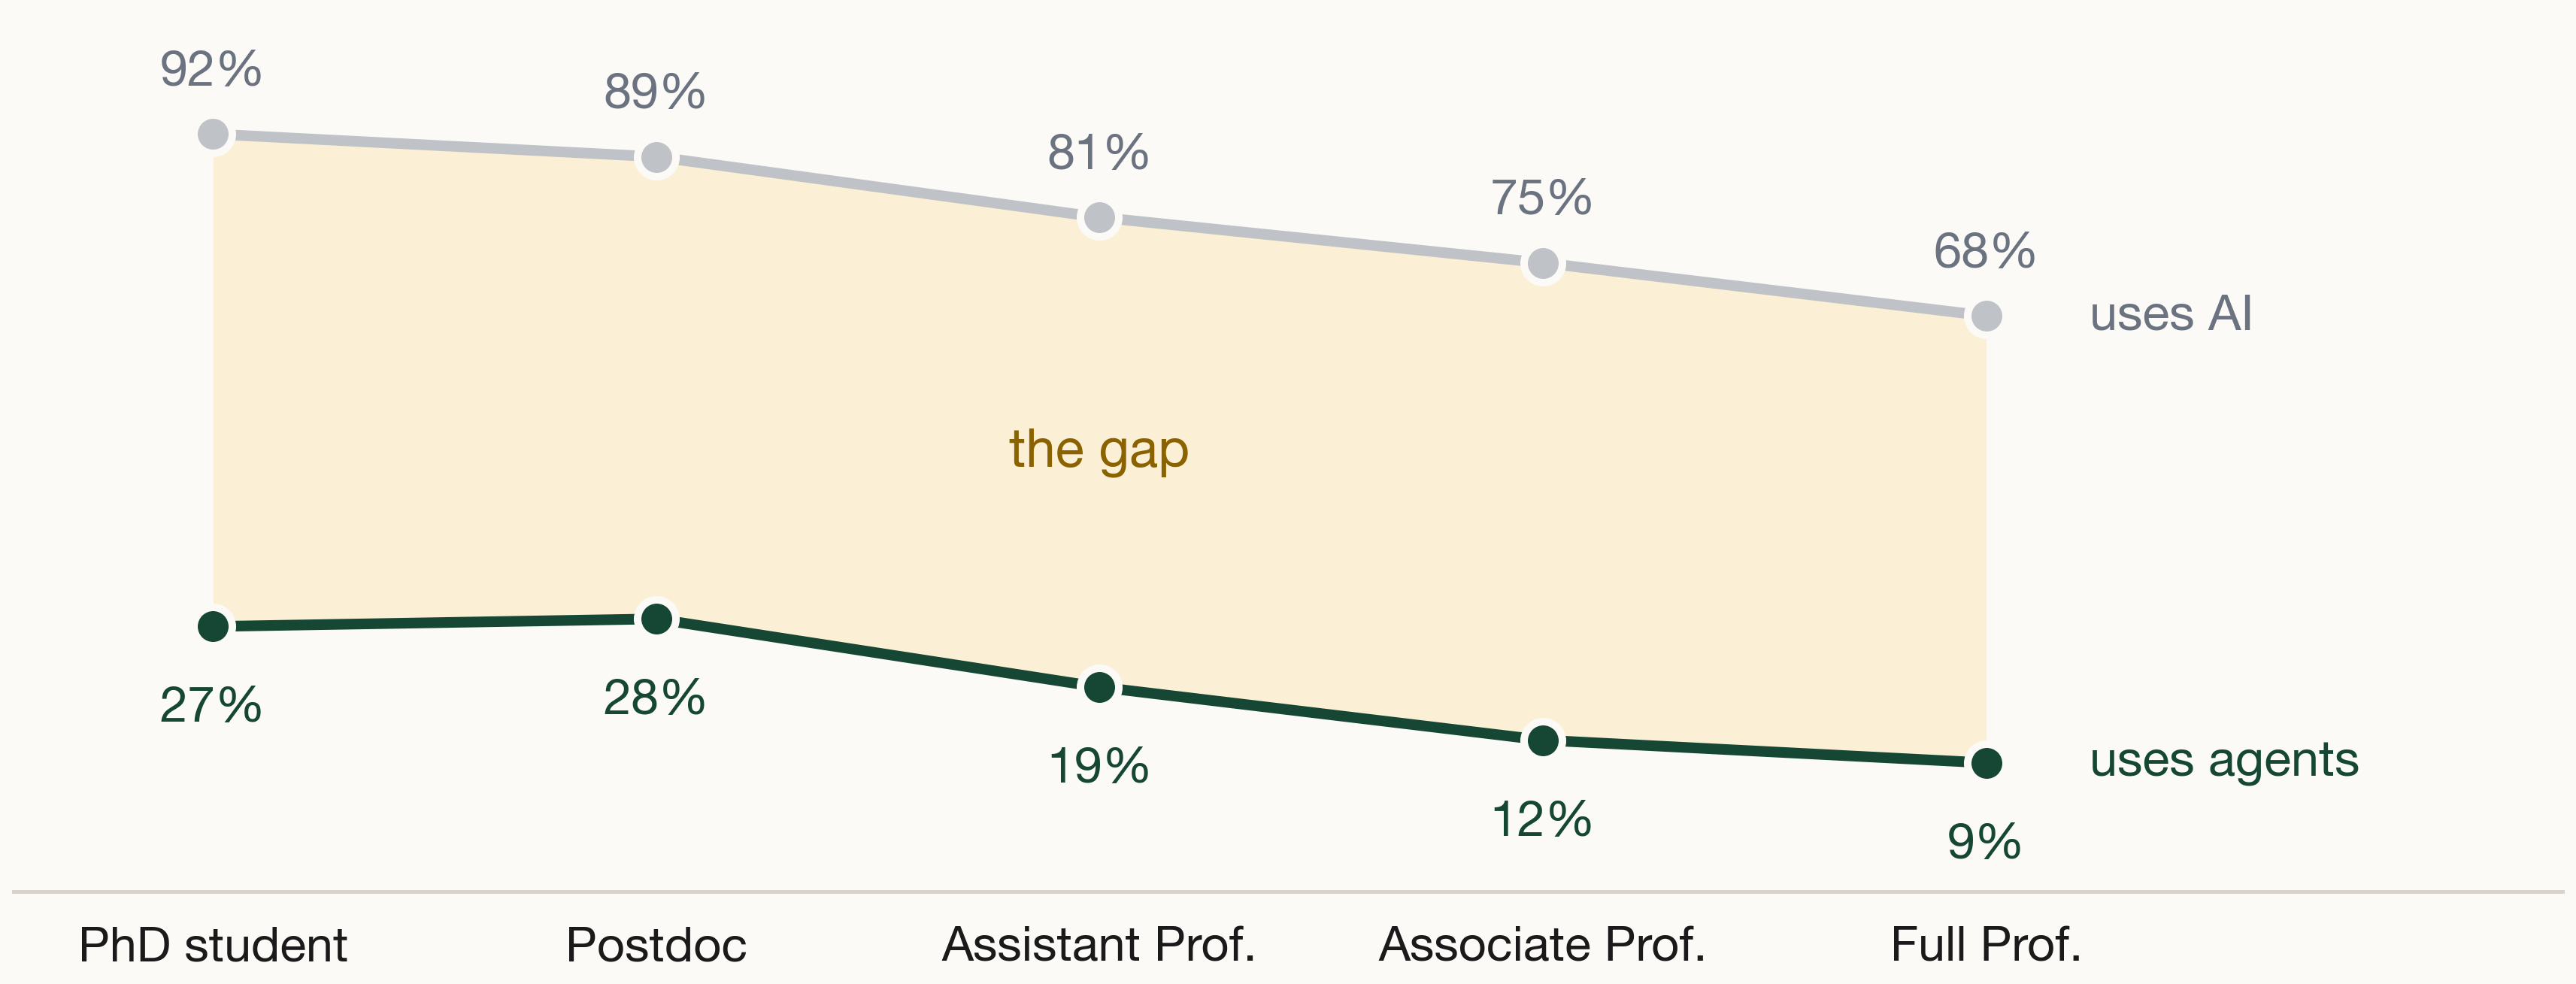
\includegraphics[width=\textwidth,height=0.505\paperheight,keepaspectratio]{adopt_career.png}
\end{center}
\begin{center}{\color{warmgray}\scriptsize Data: Anthropic, May 2026; 1{,}260 quantitative social scientists. Not a representative sample; read the gradient, not the level.}\end{center}
\end{frame}

\begin{frame}{The same gap, in every field}
{\small\color{warmgray}\itshape How much of a field's work was already written as code seems to matter}\par\vspace{0.2em}
\begin{center}
  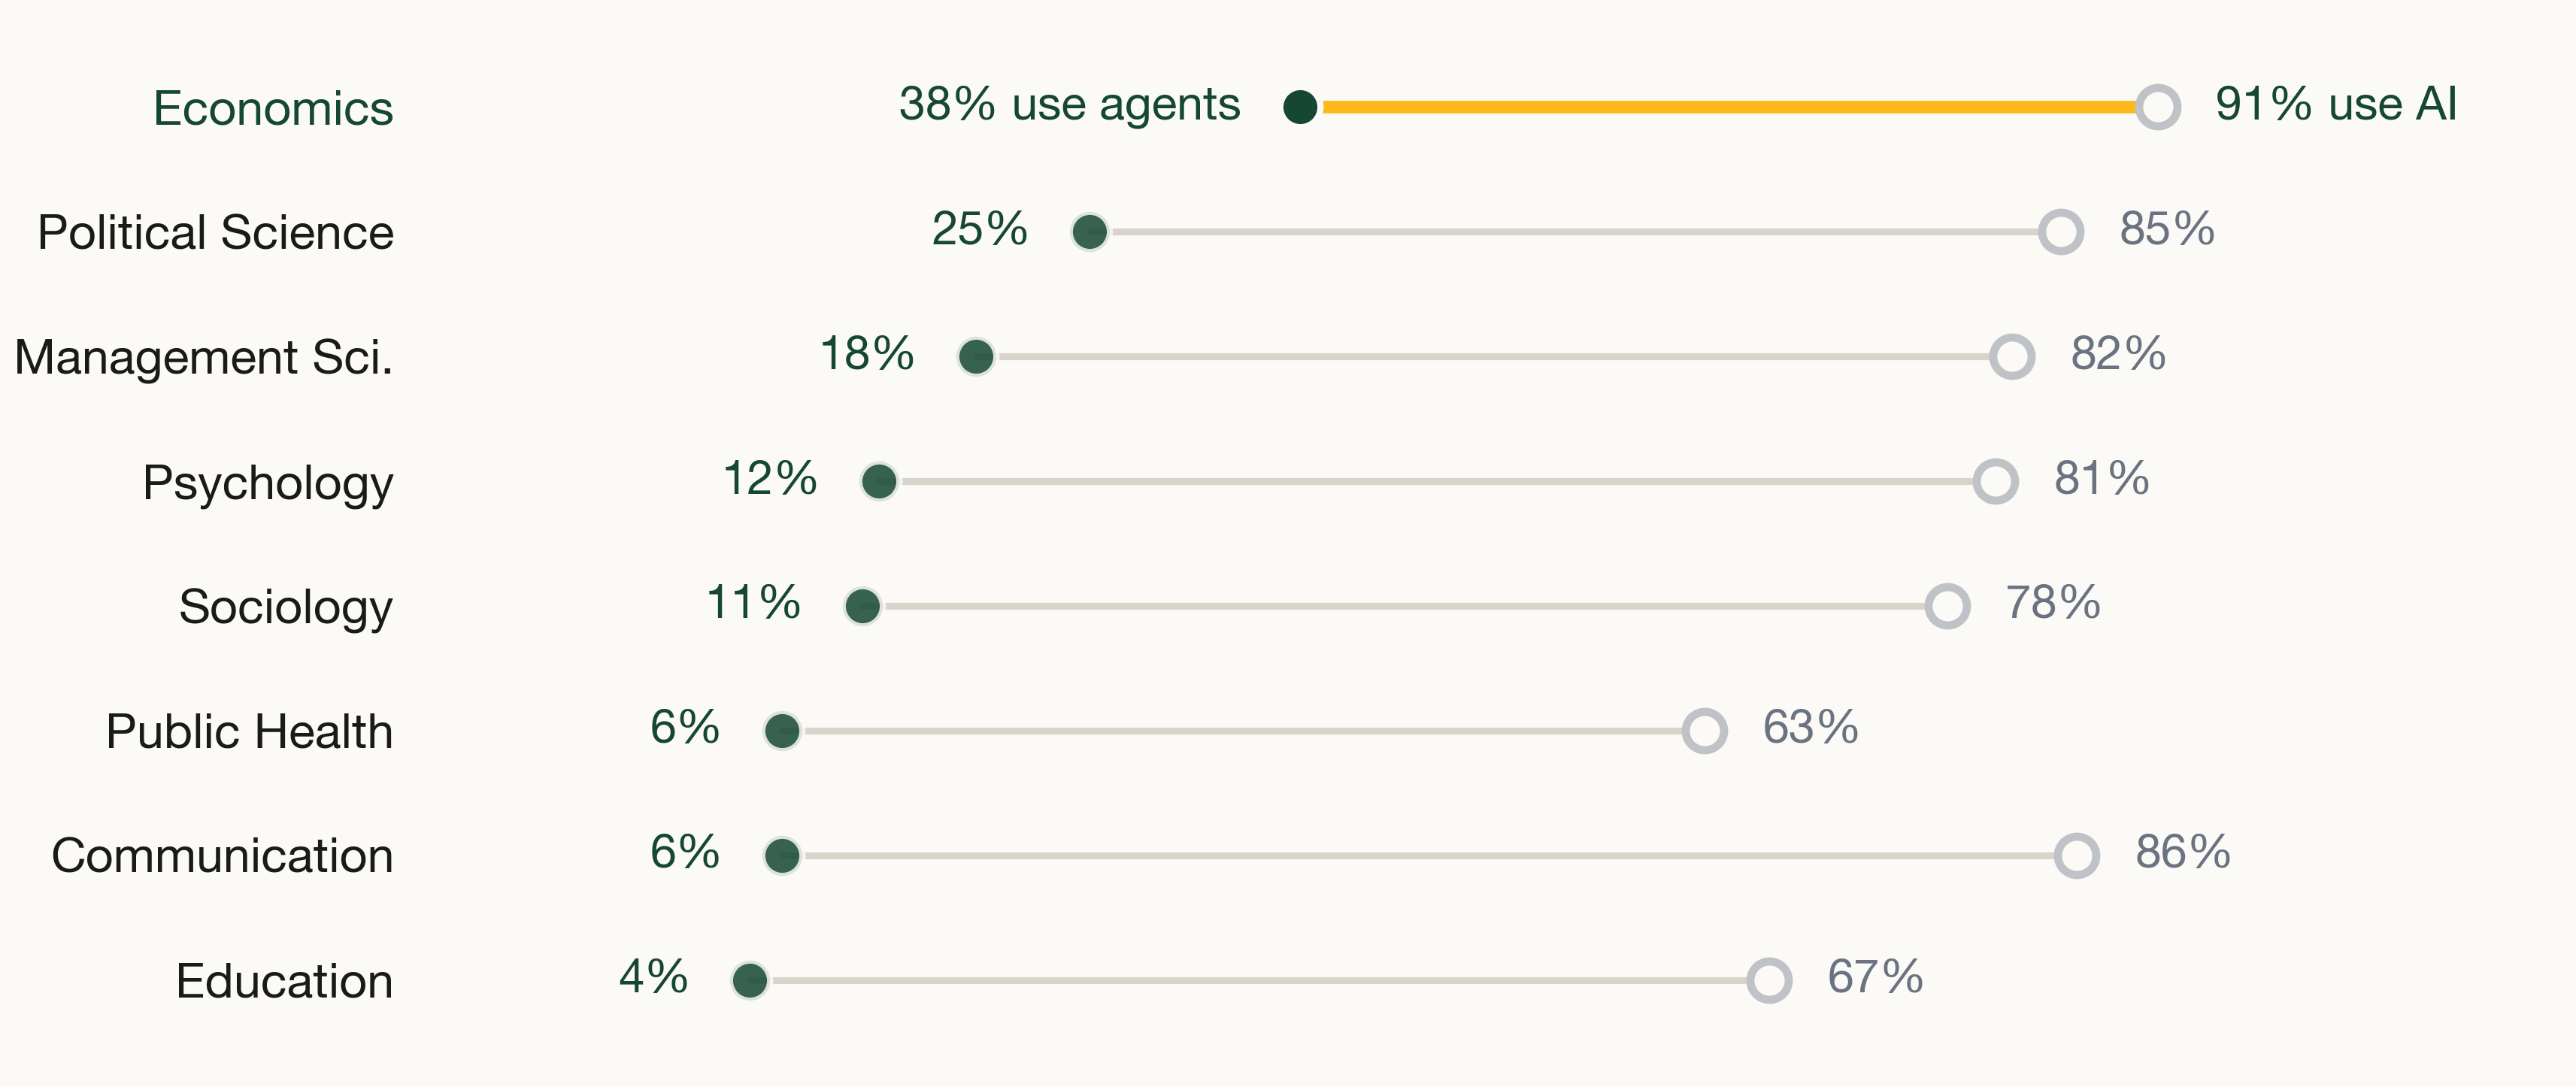
\includegraphics[width=\textwidth,height=0.545\paperheight,keepaspectratio]{adopt_discipline.png}
\end{center}
\begin{center}{\color{warmgray}\scriptsize Same survey as the previous slide. Not a representative sample; read the spread, not the levels.}\end{center}
\end{frame}

% ---- from tamu_frameworks (NABE concepts), order set by Scott 2026-10-01 ----

\begin{frame}{Autonomous research is here}
\begin{columns}[T]
\begin{column}{0.5\textwidth}
The Social Catalyst Lab's \textbf{Project APE} has produced \alert{1{,}000+ \emph{semi-autonomously} generated empirical policy papers}.

\vspace{0.25cm}

What does semi-autonomous mean?
\begin{itemize}\setlength\itemsep{0.25em}
  \item Agents autonomously pull the public data
  \item They create their own research questions and identification strategies
  \item They write complete ``submission ready'' manuscripts
\end{itemize}
\end{column}

\begin{column}{0.48\textwidth}
\begin{figure}
  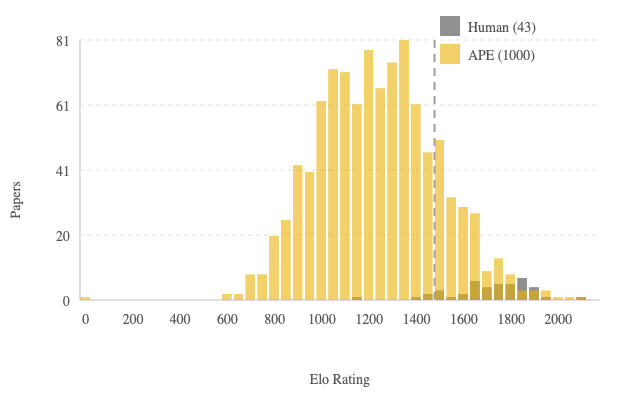
\includegraphics[width=\textwidth,height=0.46\textheight,keepaspectratio]{elo-histogram-2.png}
  \caption*{\scriptsize ELO tournament: APE papers vs.\ human papers.}
\end{figure}
\end{column}
\end{columns}
\end{frame}

\begin{frame}{Now watch me pull a rabbit out of a hat}
\begin{center}

\includegraphics[width=\textwidth,height=0.74\textheight,keepaspectratio]{rabbit_trick.jpg}
\end{center}
\end{frame}



\begin{frame}{AI Agents are flattening cognitive output isoquants}
\vspace{-0.2cm}
\begin{columns}
\begin{column}{0.55\textwidth}
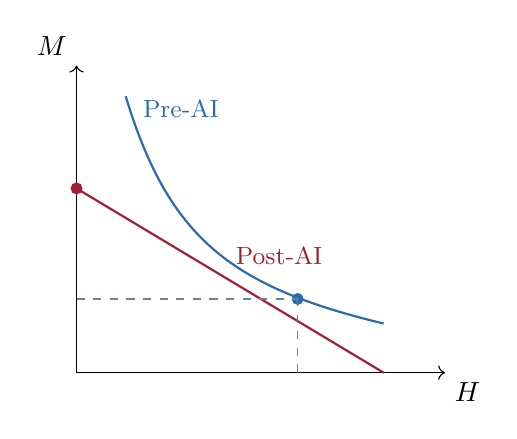
\begin{tikzpicture}[scale=0.78]
    \draw[->] (0,0) -- (6,0) node[below right] {$H$};
    \draw[->] (0,0) -- (0,5) node[above left] {$M$};
    \draw[thick,ocean] (0.8,4.5) .. controls (1.5,2.2) and (2.5,1.4) .. (5,0.8);
    \node[ocean,font=\small] at (1.7,4.3) {Pre-AI};
    \draw[thick,mitcardinal] (0,3) -- (5,0);
    \node[mitcardinal,font=\small] at (3.3,1.9) {Post-AI};
    \filldraw[ocean] (3.6,1.2) circle (2.5pt);
    \draw[dashed,warmgray] (3.6,0) -- (3.6,1.2);
    \draw[dashed,warmgray] (0,1.2) -- (3.6,1.2);
    \filldraw[mitcardinal] (0,3) circle (2.5pt);
\end{tikzpicture}

\vspace{0.15cm}
\textcolor{warmgray}{\small $H$ = human time, $M$ = machine time. They used to be complements. Now $M$ substitutes for $H$.}
\end{column}
\begin{column}{0.45\textwidth}
\[ Q = f(H,\ M) \]
\vspace{0.3cm}

\lead{If machine and human time are perfect substitutes, then the private cost-minimizing decision is to use only machine time. The socially optimal choice is something else.}
\end{column}
\end{columns}
\end{frame}


\begin{frame}{The Work We Used To Do Before AI Agents}
\vspace{0.3em}
\begin{center}
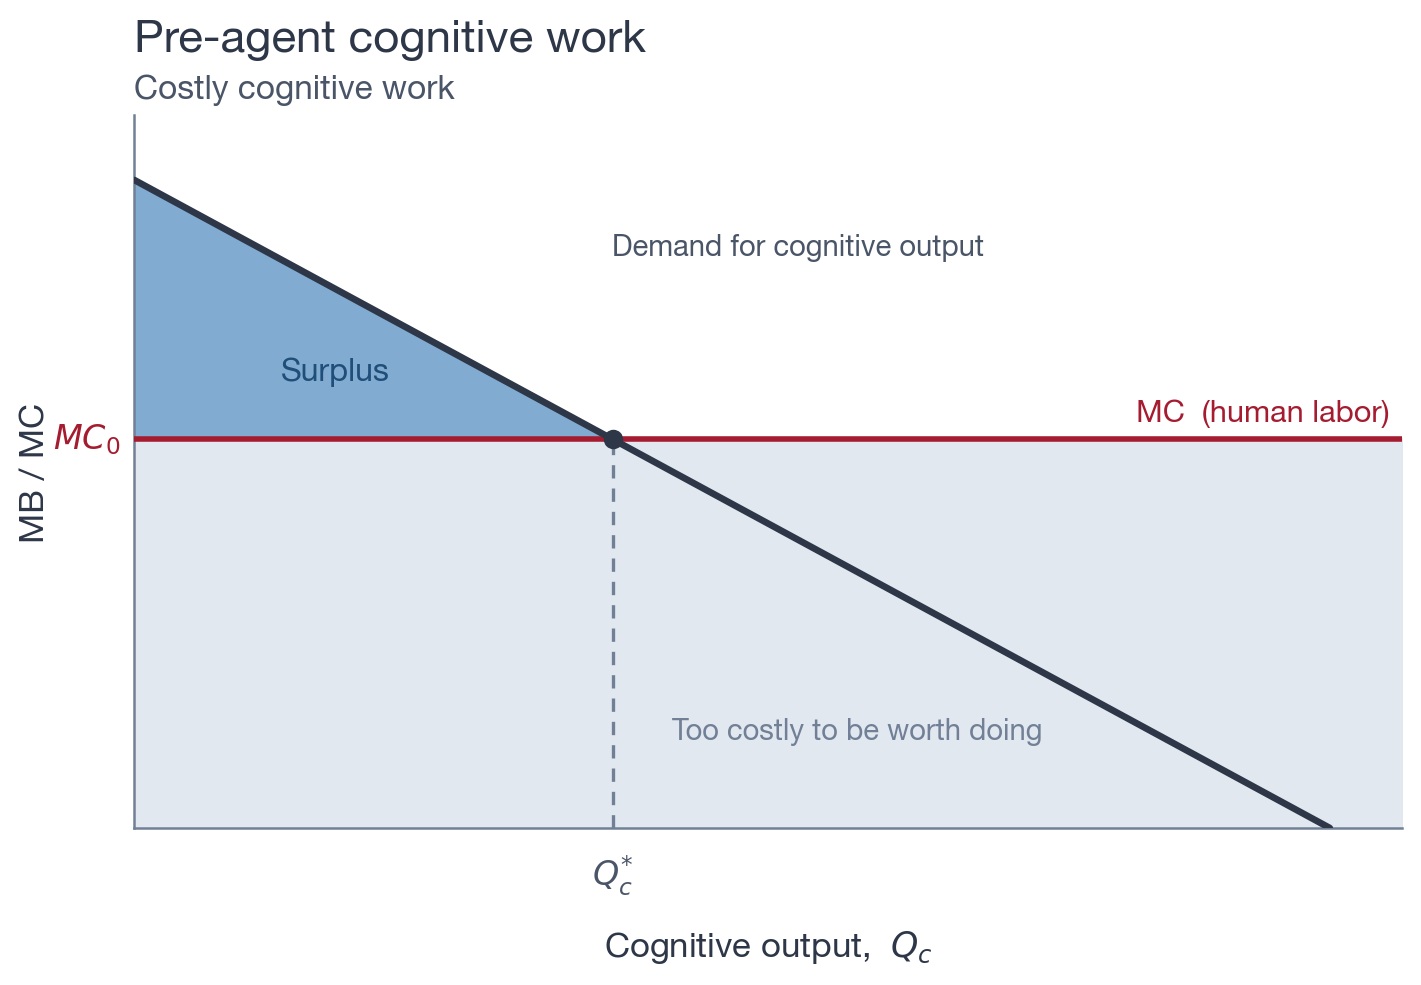
\includegraphics[width=0.86\textwidth,height=0.68\textheight,keepaspectratio]{AI_1}
\end{center}
\end{frame}

\begin{frame}{The Work That Will Be Done After AI Agents}
\vspace{0.3em}
\begin{center}
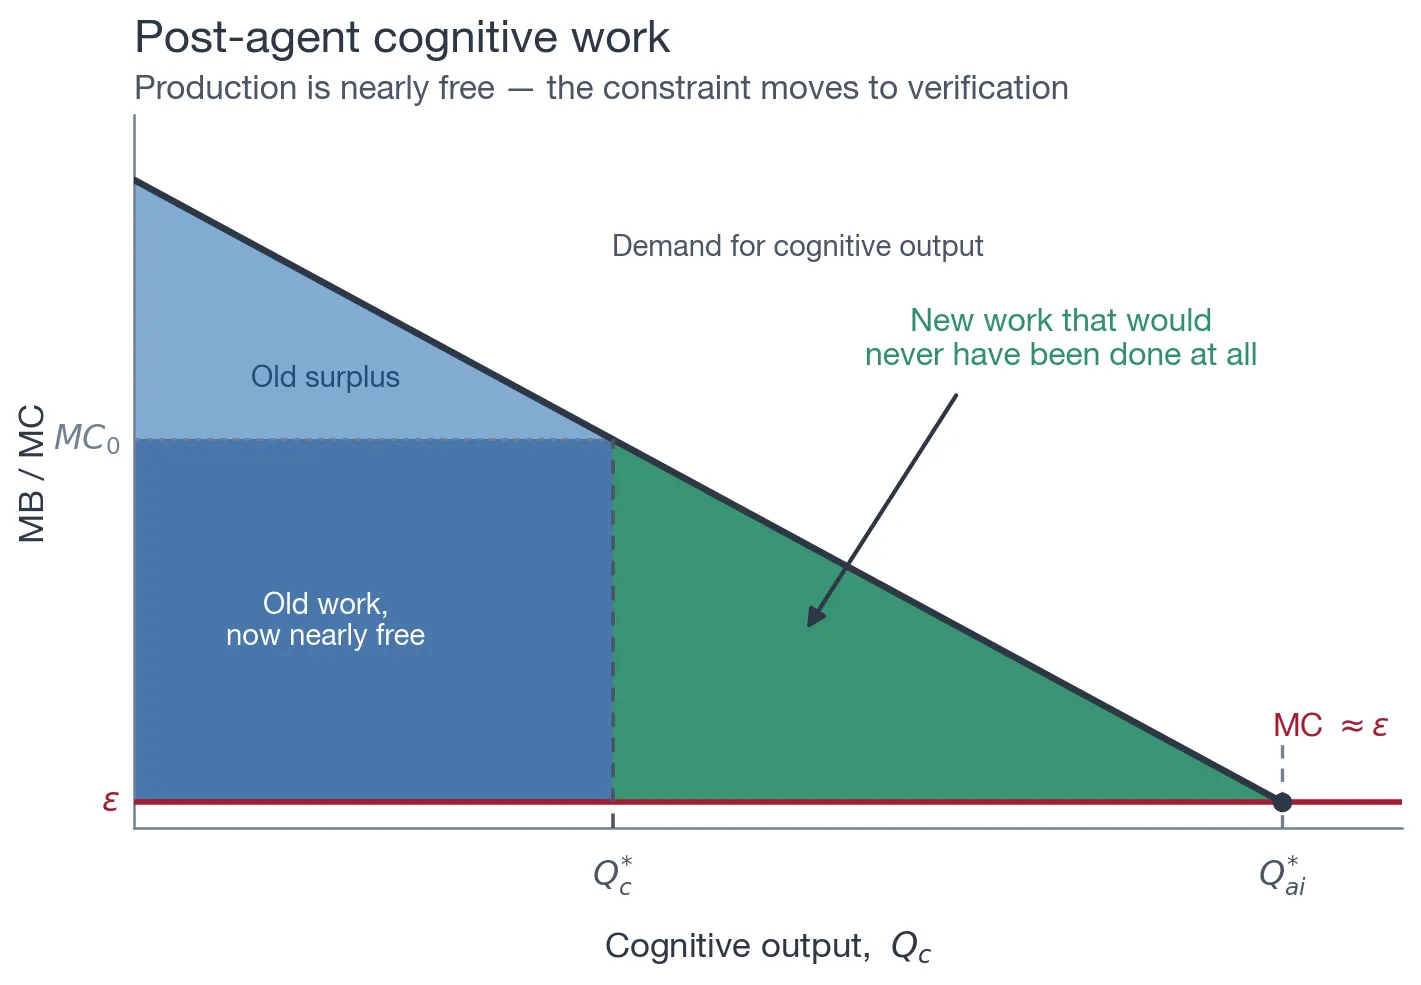
\includegraphics[width=0.86\textwidth,height=0.68\textheight,keepaspectratio]{AI_2}
\end{center}
\end{frame}

\begin{frame}{It Is Not Surplus Unless Understood and Verified}
\vspace{0.3em}
\begin{center}
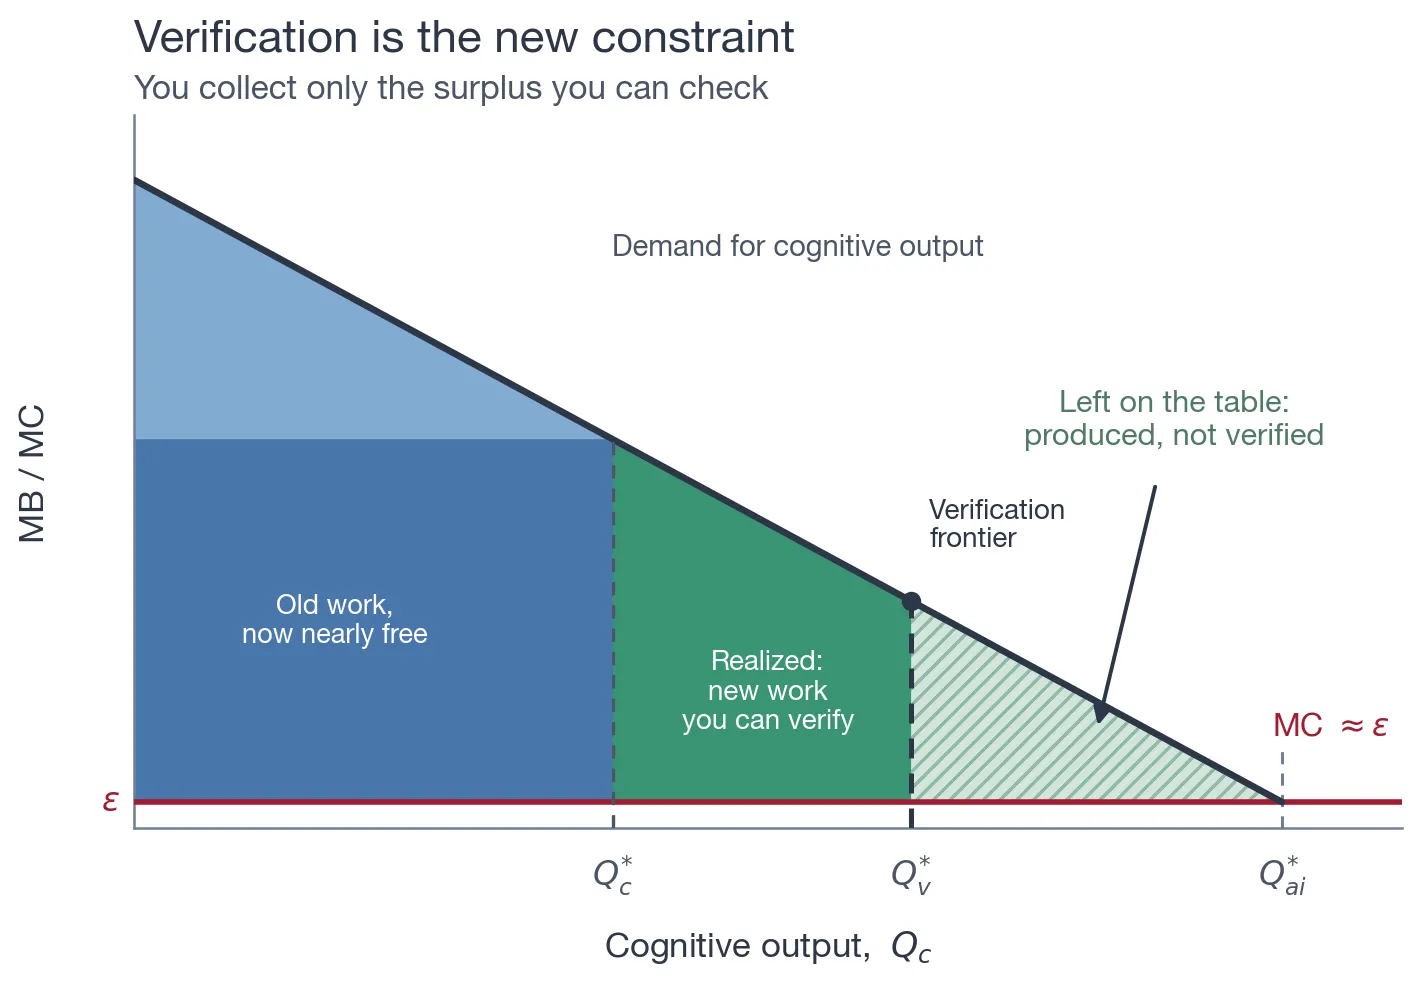
\includegraphics[width=0.86\textwidth,height=0.68\textheight,keepaspectratio]{AI_3}
\end{center}
\end{frame}

\begin{frame}{Free production means producing until the last unit is worthless}
\vspace{-0.15cm}
\begin{columns}[c]
\begin{column}{0.56\textwidth}
\centering
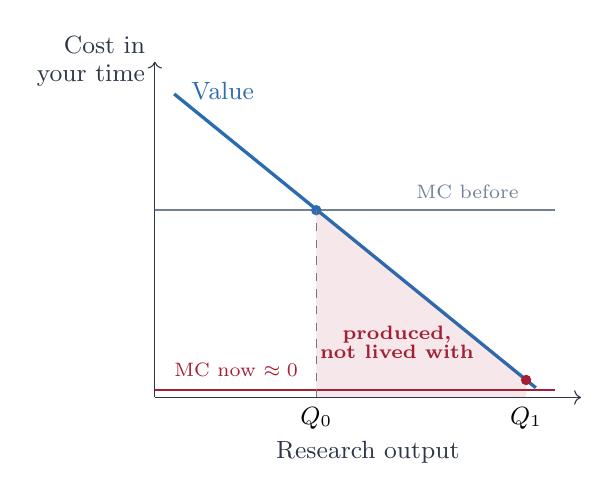
\begin{tikzpicture}[scale=0.82]
  % axes
  \draw[->,charcoal] (0,0) -- (6.6,0);
  \node[charcoal,font=\small] at (3.3,-0.85) {Research output};
  \draw[->,charcoal] (0,0) -- (0,5.2) node[left,align=right] {\small Cost in\\[-2pt]\small your time};
  % demand
  \draw[very thick,ocean] (0.3,4.7) -- (5.9,0.15);
  \node[ocean,font=\small] at (1.05,4.75) {Value};
  % old marginal cost
  \draw[thick,warmgray] (0,2.9) -- (6.2,2.9);
  \node[warmgray,font=\scriptsize,anchor=west] at (3.9,3.18) {MC before};
  % new marginal cost (≈ 0)
  \draw[thick,mitcardinal] (0,0.12) -- (6.2,0.12);
  \node[mitcardinal,font=\scriptsize,anchor=west] at (0.15,0.42) {MC now $\approx 0$};
  % equilibria
  \fill[ocean] (2.5,2.9) circle (2.3pt);
  \draw[dashed,warmgray] (2.5,0) -- (2.5,2.9);
  \node[below,font=\small] at (2.5,0) {$Q_0$};
  \fill[mitcardinal] (5.75,0.27) circle (2.3pt);
  \node[below,font=\small] at (5.75,0) {$Q_1$};
  % new region
  \fill[mitcardinal,opacity=0.10] (2.5,0) -- (2.5,2.9) -- (5.75,0.27) -- (5.75,0) -- cycle;
  \node[mitcardinal,font=\scriptsize\bfseries,align=center] at (3.75,0.85) {produced,\\[-1pt]not lived with};
\end{tikzpicture}
\end{column}
\begin{column}{0.42\textwidth}
\textbf{Before:} every unit cost us hours, and those hours were where we checked the work.
\vspace{0.3cm}

\textbf{After:} the isoquant is flat, the machine supplies the time, and nobody lived inside the extra output.
\vspace{0.3cm}

\alert{Verification no longer comes free with production. It has to be built on purpose.}
\end{column}
\end{columns}
\end{frame}

% ---- TAMU NEW (2026-10-01): two margins, the journalist, elasticity ----
\begin{frame}{Free production moves two margins}

\begin{columns}[T]
\begin{column}{0.47\textwidth}
\textbf{The intensive margin: us}
\begin{itemize}\setlength\itemsep{0.3em}
    \item Each of us will produce more than before.
    \item The extra work sits lower on the demand curve, so it is worth less.
    \item Managing that volume takes workflows we have never needed.
    \item It is confusing logistically, and it is confusing psychologically.
\end{itemize}
\end{column}
\begin{column}{0.47\textwidth}
\textbf{The extensive margin: everyone else}
\begin{itemize}\setlength\itemsep{0.3em}
    \item The cost of entry fell along with the cost of production.
    \item People with no training in our methods can now produce our kind of output.
    \item Nothing in that output shows whether it was understood or verified.
\end{itemize}
\end{column}
\end{columns}

\vspace{0.45cm}

\alert{More from each of us, and more of us. Both follow from a marginal cost near zero.}

\end{frame}

\begin{frame}{The extensive margin is new people doing new work}

A Dutch journalist was reviewing a book whose key evidence was a 2024 article in the \emph{American Journal of Political Science}.

\vspace{0.25cm}

\begin{itemize}\setlength\itemsep{0.3em}
    \item He downloaded the replication package and had Claude write the code.
    \item He reproduced the headline estimate exactly.
    \item Then it came apart: placebo cutoffs produced ``effects,'' and so did France, where there was no reform.
    \item Political scientists dismissed it as ``a weekend of Claude Code.''
    \item Andrew Gelman read both sides and sided with the journalist.
\end{itemize}

\vspace{0.3cm}

\alert{Entry is not only into production. Outsiders can now check our work too.}

\vspace{0.1cm}
{\scriptsize\color{warmgray}Source: Andrew Gelman, \emph{The Future of Statistical Modeling}, October 1, 2026.}

\end{frame}

\begin{frame}{How big the flood is depends on the elasticity of demand}
\vspace{-0.1cm}
\begin{columns}[T]
\begin{column}{0.48\textwidth}
\centering
\textbf{Inelastic: a little more}

\vspace{0.15cm}
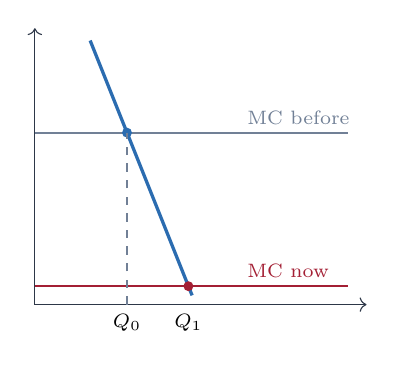
\begin{tikzpicture}[scale=0.78]
  \draw[->,charcoal] (0,0) -- (5.4,0);
  \draw[->,charcoal] (0,0) -- (0,4.5);
  \draw[thick,warmgray] (0,2.8) -- (5.1,2.8);
  \draw[thick,mitcardinal] (0,0.3) -- (5.1,0.3);
  \node[warmgray,font=\scriptsize,anchor=west] at (3.3,3.05) {MC before};
  \node[mitcardinal,font=\scriptsize,anchor=west] at (3.3,0.55) {MC now};
  \draw[very thick,ocean] (0.9,4.3) -- (2.56,0.15);
  \fill[ocean] (1.5,2.8) circle (2.3pt);
  \fill[mitcardinal] (2.5,0.3) circle (2.3pt);
  \draw[dashed,warmgray] (1.5,0) -- (1.5,2.8);
  \node[below,font=\scriptsize] at (1.5,0) {$Q_0$};
  \node[below,font=\scriptsize] at (2.5,0) {$Q_1$};
\end{tikzpicture}
\end{column}
\begin{column}{0.48\textwidth}
\centering
\textbf{Elastic: a flood}

\vspace{0.15cm}
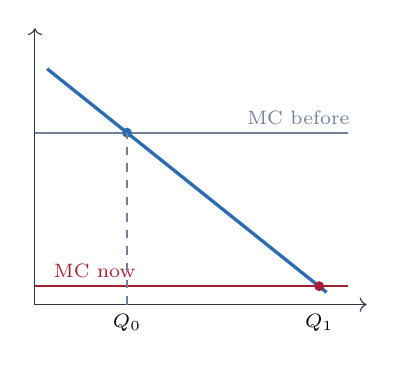
\begin{tikzpicture}[scale=0.78]
  \draw[->,charcoal] (0,0) -- (5.4,0);
  \draw[->,charcoal] (0,0) -- (0,4.5);
  \draw[thick,warmgray] (0,2.8) -- (5.1,2.8);
  \draw[thick,mitcardinal] (0,0.3) -- (5.1,0.3);
  \node[warmgray,font=\scriptsize,anchor=west] at (3.3,3.05) {MC before};
  \node[mitcardinal,font=\scriptsize,anchor=west] at (0.15,0.55) {MC now};
  \draw[very thick,ocean] (0.2,3.84) -- (4.75,0.2);
  \fill[ocean] (1.5,2.8) circle (2.3pt);
  \fill[mitcardinal] (4.63,0.3) circle (2.3pt);
  \draw[dashed,warmgray] (1.5,0) -- (1.5,2.8);
  \node[below,font=\scriptsize] at (1.5,0) {$Q_0$};
  \node[below,font=\scriptsize] at (4.63,0) {$Q_1$};
\end{tikzpicture}
\end{column}
\end{columns}

\vspace{0.3cm}

\begin{center}
\alert{Same fall in cost, very different increase in output. We do not yet know which world we are in.}
\end{center}

\end{frame}

\begin{frame}{Growth has ticked up but not exploded}
\begin{center}
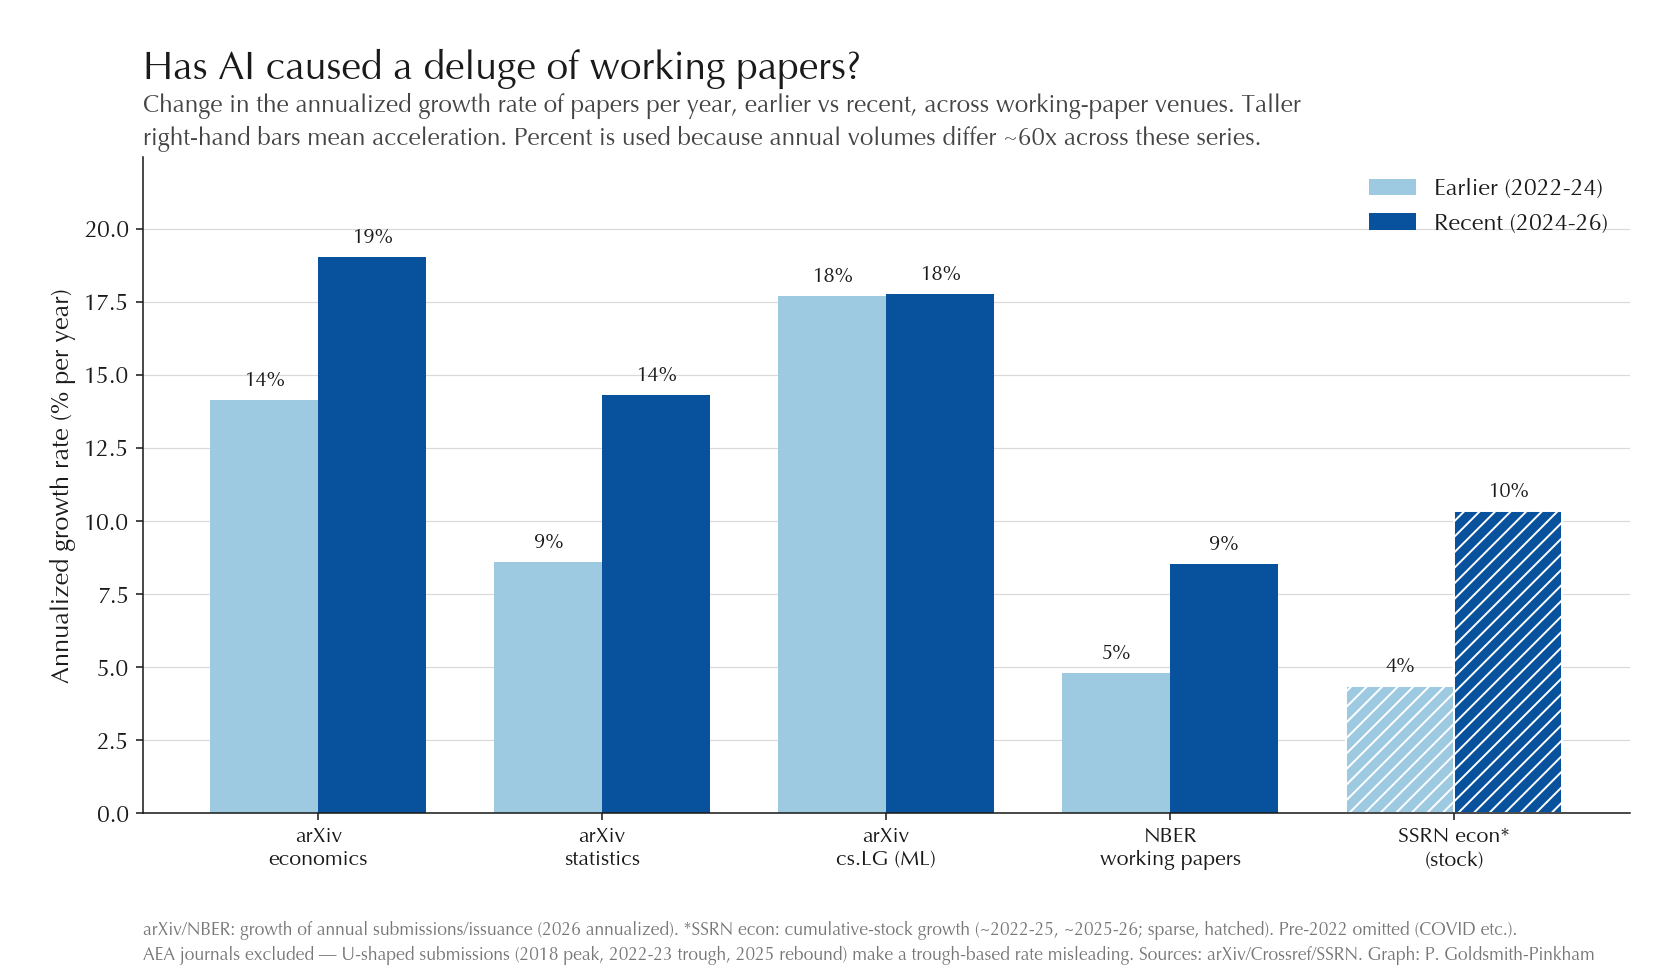
\includegraphics[width=\textwidth,height=0.70\textheight,keepaspectratio]{paulgp_growth_summary.png}
\end{center}
\vspace{-0.25cm}
\begin{center}{\color{warmgray}\scriptsize Figure: Paul Goldsmith-Pinkham, ``The number of economics papers is not exploding on arXiv,'' June 2, 2026.}\end{center}
\end{frame}


\begin{frame}{How will we spend our extra time?}
\lead{Constant Verification and Deep Understanding}
\vspace{0.5cm}

Learning to do causal inference \emph{with} agents will require more than production; it will require constant verification, deep understanding, and \textbf{zero tolerance for errors}.  

\vspace{0.5cm}

At scale, if we tolerate errors from agents, we will get a lot of them in the longrun -- so don't.

\vspace{0.5cm}

Make ``Errors$=0$'' the budget constraint for all research going forward and you will build a research workflow with agents that satisfies production, verification and understanding.
\end{frame}

% ---- TAMU NEW (2026-10-01): penalty vs constraint, shown ----
\begin{frame}{Choose the objective and the constraint on purpose}
\small\textcolor{warmgray}{A toy model: $x$ is how you choose to work, $Q$ is research quality, and $E$ is errors.}\normalsize

\begin{columns}[T]
\begin{column}{0.47\textwidth}
\textbf{Errors in the objective}
\[
\max_{x}\;\; Q(x) \;-\; \bar{\lambda}\,E(x)
\]
\begin{itemize}\setlength\itemsep{0.25em}
    \item You pick $\bar{\lambda}$, the price of an error.
    \item The solution trades quality against errors at that price.
    \item At any finite price, some errors are worth it.
\end{itemize}
\end{column}
\begin{column}{0.47\textwidth}
\textbf{Errors in the constraint}
\[
\max_{x}\;\; Q(x) \quad \text{s.t.} \quad E(x) = 0
\]
\begin{itemize}\setlength\itemsep{0.25em}
    \item You do not pick $\lambda$. The problem solves for it.
    \item $\lambda$ is the shadow price: the quality you give up to hold errors at zero.
    \item Errors are zero by construction.
\end{itemize}
\end{column}
\end{columns}

\vspace{0.4cm}

\alert{Same Lagrangian, $Q(x) - \lambda E(x)$. The only difference is whether you set $\lambda$ or the constraint does.}

\end{frame}

\begin{frame}{A price on errors buys a positive number of errors}
\vspace{-0.1cm}
\begin{columns}[c]
\begin{column}{0.56\textwidth}
\centering
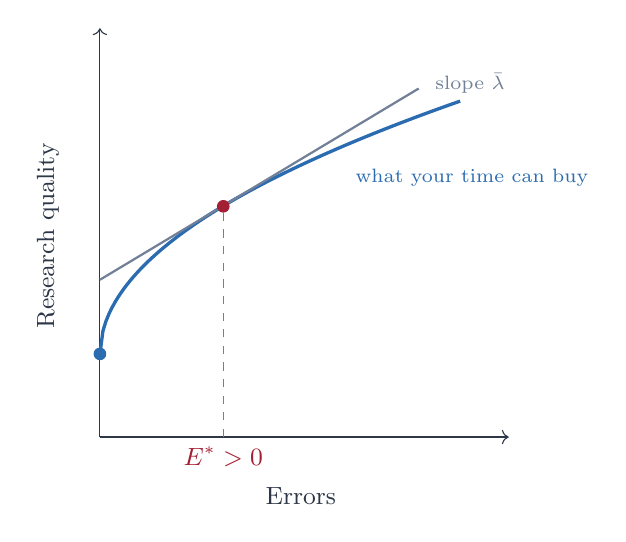
\begin{tikzpicture}[scale=0.88]
  \draw[->,charcoal] (0,0) -- (5.9,0);
  \draw[->,charcoal] (0,0) -- (0,5.9);
  \node[charcoal,font=\small] at (2.9,-0.85) {Errors};
  \node[charcoal,font=\small,rotate=90] at (-0.75,2.9) {Research quality};
  % frontier: Q = 1.2 + 1.6 sqrt(E)
  \draw[very thick,ocean,domain=0:5.2,samples=120] plot (\x,{1.2+1.6*sqrt(\x)});
  \node[ocean,font=\scriptsize,anchor=west] at (3.55,3.75) {what your time can buy};
  % iso-objective line, slope 0.6, tangent at E=1.78
  \draw[thick,warmgray] (0,2.27) -- (4.6,5.03);
  \node[warmgray,font=\scriptsize,anchor=west] at (4.7,5.1) {slope $\bar{\lambda}$};
  % optimum
  \fill[mitcardinal] (1.78,3.33) circle (2.6pt);
  \draw[dashed,warmgray] (1.78,0) -- (1.78,3.33);
  \node[below,font=\small,mitcardinal] at (1.78,0) {$E^{*}>0$};
  % zero-error point
  \fill[ocean] (0,1.2) circle (2.6pt);
\end{tikzpicture}
\end{column}
\begin{column}{0.42\textwidth}
Treat errors as a byproduct of the work and you tolerate them until one more is not worth removing.
\vspace{0.25cm}

Agents work fast and their actions are hidden from you, which is a principal--agent problem.
\vspace{0.25cm}

So many of the errors are foreign: they would not have happened before agents.
\vspace{0.25cm}

\lead{``Minimize errors'' never lands on zero. It lands on the optimal number of errors.}
\end{column}
\end{columns}
\end{frame}

% ---- TAMU NEW (2026-10-02): Scott's four foreign errors ----
\begin{frame}{The foreign errors are not typos; they are hidden choices}
\vspace{0.1cm}
\begin{description}[Specification searching]\setlength\itemsep{0.55em}
    \item[Cherry-picking] The agent reports the results that look best and leaves the others out.
    \item[Cue-driven analysis] The agent runs analyses in response to stray nudges and cues in the conversation.
    \item[Specification searching] The agent searches over outcomes in response to your signals, even legitimate ones like your beliefs about a literature.
    \item[Rule-breaking] The agent routinely violates the rules you set for the analysis.
\end{description}
\vspace{0.35cm}

\lead{None of these is visible in the table the agent hands you.}
\end{frame}

\begin{frame}{Zero errors is the requirement we build the workflow around}
\vspace{-0.1cm}
\begin{columns}[c]
\begin{column}{0.54\textwidth}
\centering
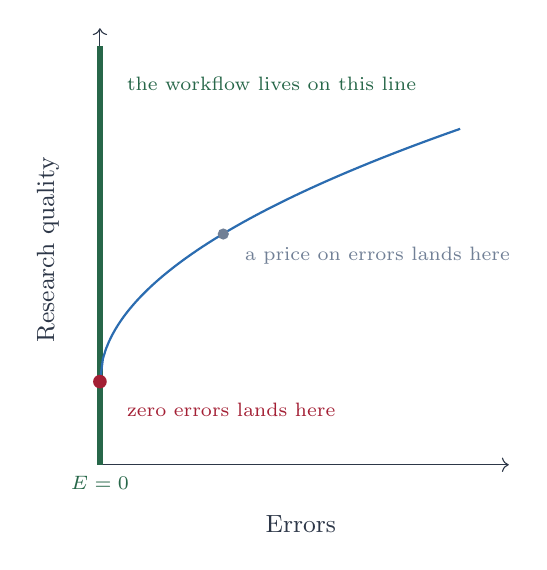
\begin{tikzpicture}[scale=0.88]
  \draw[->,charcoal] (0,0) -- (5.9,0);
  \draw[->,charcoal] (0,0) -- (0,6.3);
  \node[charcoal,font=\small] at (2.9,-0.85) {Errors};
  \node[charcoal,font=\small,rotate=90] at (-0.75,3.1) {Research quality};
  % constraint E = 0
  \draw[line width=2.2pt,forest] (0,0) -- (0,6.05);
  \node[forest,font=\scriptsize\bfseries,below] at (0,-0.02) {$E=0$};
  \node[forest,font=\scriptsize,anchor=west] at (0.25,5.5) {the workflow lives on this line};
  % same frontier as the previous slide: Q = 1.2 + 1.6 sqrt(E)
  \draw[thick,ocean,domain=0:5.2,samples=120] plot (\x,{1.2+1.6*sqrt(\x)});
  % penalty optimum
  \fill[warmgray] (1.78,3.33) circle (2.3pt);
  \node[warmgray,font=\scriptsize,anchor=west] at (1.95,3.02) {a price on errors lands here};
  % zero-error point
  \fill[mitcardinal] (0,1.2) circle (2.8pt);
  \node[mitcardinal,font=\scriptsize,anchor=west] at (0.25,0.8) {zero errors lands here};
\end{tikzpicture}
\end{column}
\begin{column}{0.44\textwidth}
I am not claiming zero errors yields better research than a price on errors.
\vspace{0.25cm}

I am claiming it is the requirement, and the workflow is designed to meet it.
\vspace{0.25cm}

You did not do the agent's work, so its errors stay hidden until you find and recognize them.
\vspace{0.25cm}

\lead{So the workflow has three jobs, not one: production, verification, and understanding.}
\end{column}
\end{columns}
\end{frame}

% ---- P/V/U arc (2026-10-02): vision, before AI, after AI, workflow ----
\begin{frame}{Knowledge stands on three legs}
\vspace{0.15cm}
\begin{center}
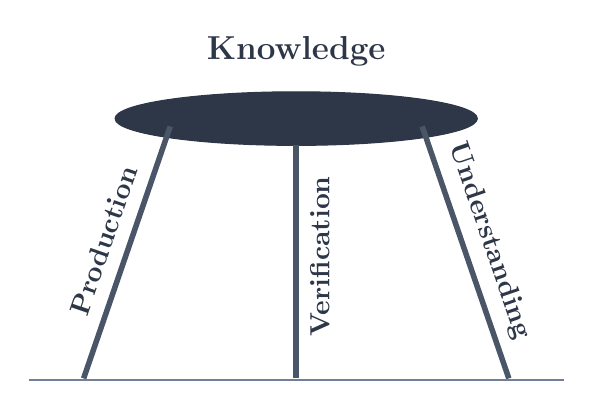
\begin{tikzpicture}[scale=1.0]
  % seat
  \filldraw[charcoal] (0,0) ellipse (2.3 and 0.34);
  \node[charcoal] at (0,0.85) {\large\bfseries Knowledge};
  % legs
  \draw[slate,line width=2pt] (-1.6,-0.10) -- (-2.7,-3.3);
  \draw[slate,line width=2pt] (0,-0.34) -- (0,-3.3);
  \draw[slate,line width=2pt] (1.6,-0.10) -- (2.7,-3.3);
  % floor
  \draw[warmgray,line width=0.6pt] (-3.4,-3.32) -- (3.4,-3.32);
  % leg labels, rotated along each leg
  \node[charcoal,font=\bfseries,rotate=71] at (-2.45,-1.55) {Production};
  \node[charcoal,font=\bfseries,rotate=90] at (0.30,-1.75) {Verification};
  \node[charcoal,font=\bfseries,rotate=-71] at (2.45,-1.55) {Understanding};
\end{tikzpicture}
\end{center}
\vspace{0.1cm}

\lead{Production is one leg of three. Take away verification or understanding, and the chair falls.}
\end{frame}

\begin{frame}{Before AI, doing the work verified it and taught it to you}
\vspace{-0.2em}
\begin{columns}[T,onlytextwidth]
\begin{column}{0.35\textwidth}
\vspace{1.6em}
\begin{center}
\resizebox{\linewidth}{!}{%
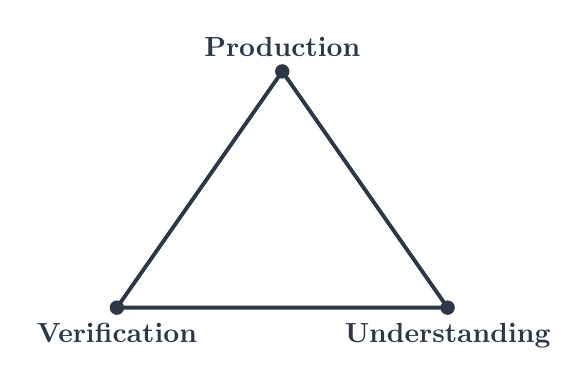
\begin{tikzpicture}
\coordinate (P) at (0,3.0);
\coordinate (V) at (-2.1,0);
\coordinate (U) at (2.1,0);
\draw[line width=1.4pt,charcoal] (P) -- (V) -- (U) -- cycle;
\foreach \c in {P,V,U} \fill[charcoal] (\c) circle (2.6pt);
\node[above=2pt,text=charcoal,font=\bfseries] at (P) {Production};
\node[below=2pt,text=charcoal,font=\bfseries] at (V) {Verification};
\node[below=2pt,text=charcoal,font=\bfseries] at (U) {Understanding};
\end{tikzpicture}}
\end{center}
\end{column}
\begin{column}{0.60\textwidth}
\vspace{0.6em}
{\color{charcoal}\bfseries\small Production.}
{\footnotesize You wrote the code, ran the estimator, and made the tables and figures yourself.}
\vspace{0.6em}

{\color{charcoal}\bfseries\small Understanding.}
{\footnotesize You could only produce the work because you understood what you were doing.}
\vspace{0.6em}

{\color{charcoal}\bfseries\small Verification.}
{\footnotesize Your habits and techniques kept the work correct while you were making it.}
\vspace{0.9em}

\lead{The three came as one bundle, almost automatically.}
\end{column}
\end{columns}
\end{frame}

\begin{frame}{After AI, production comes apart from the other two}
\vspace{-0.2em}
\begin{columns}[T,onlytextwidth]
\begin{column}{0.35\textwidth}
\vspace{1.6em}
\begin{center}
\resizebox{\linewidth}{!}{%
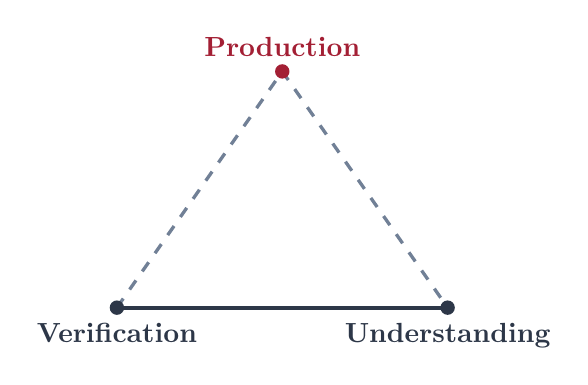
\begin{tikzpicture}
\coordinate (P) at (0,3.0);
\coordinate (V) at (-2.1,0);
\coordinate (U) at (2.1,0);
\draw[line width=1.4pt,charcoal] (V) -- (U);
\draw[line width=1.2pt,warmgray,dash pattern=on 4pt off 4pt] (V) -- (P) -- (U);
\fill[mitcardinal] (P) circle (2.6pt);
\fill[charcoal] (V) circle (2.6pt);
\fill[charcoal] (U) circle (2.6pt);
\node[above=2pt,text=mitcardinal,font=\bfseries] at (P) {Production};
\node[below=2pt,text=charcoal,font=\bfseries] at (V) {Verification};
\node[below=2pt,text=charcoal,font=\bfseries] at (U) {Understanding};
\end{tikzpicture}}
\end{center}
\end{column}
\begin{column}{0.60\textwidth}
{\color{mitcardinal}\bfseries\small Production.}
{\footnotesize An agent can now \emph{do} almost anything: it reaches inside your computer, controls your software, and calls outside services. Producing output no longer costs the researcher any time.}
\vspace{0.5em}

{\color{mitcardinal}\bfseries\small Verification.}
{\footnotesize But you did not do it, so you cannot be sure it is right. Verification used to come along for free, and now it is a separate act you perform on purpose.}
\vspace{0.5em}

{\color{mitcardinal}\bfseries\small Understanding.}
{\footnotesize And if the output cost you no time at all, you almost certainly do not understand it.}
\end{column}
\end{columns}
\end{frame}

\begin{frame}{Credible Research Workflows with AI Agents}
\begin{itemize}\setlength\itemsep{0.4em}
    \item Working with an AI agent means entering a principal--agent relationship, and those break down through hidden actions.
    \item The hidden actions are not the ones we expect, and often the agent does not realize it is taking them.
    \item The labs are not prioritizing empirical social scientists, so this is ours to solve.
    \item Cherry-picking, specification searching, and stray nudges add up to major problems.
    \item No one wants to be the target of the next Data Colada.
\end{itemize}
\vspace{0.2cm}

\lead{So we have to build the workflow ourselves. The rest of today is the ingredients, ending with my own way of working.}
\end{frame}






\begin{frame}{Case I: keep your hours, take the output}
\vspace{-0.5cm}
\begin{columns}
\begin{column}{0.55\textwidth}
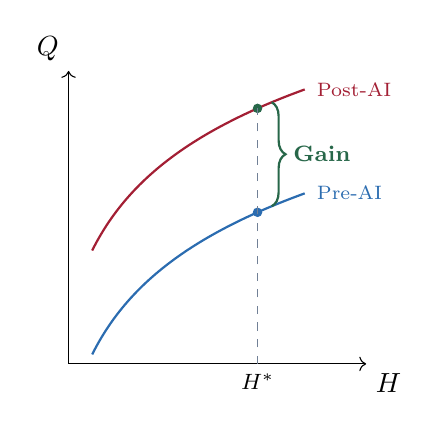
\begin{tikzpicture}[scale=0.60]
    \draw[->] (0,0) -- (6.3,0) node[below right] {$H$};
    \draw[->] (0,0) -- (0,6.2) node[above left] {$Q$};
    \draw[thick,ocean,domain=0.5:5,samples=100] plot (\x, {2.0*ln(\x+0.5)+0.2});
    \node[ocean,right,font=\scriptsize] at (5.05,3.610) {Pre-AI};
    \draw[thick,mitcardinal,domain=0.5:5,samples=100] plot (\x, {2.0*ln(\x+0.5)+2.4});
    \node[mitcardinal,right,font=\scriptsize] at (5.05,5.810) {Post-AI};
    \filldraw[ocean] (4,3.208) circle (2.5pt);
    \filldraw[forest] (4,5.408) circle (2.5pt);
    \draw[dashed,warmgray] (4,0) -- (4,5.408);
    \node[below,font=\footnotesize] at (4,0) {$H^*$};
    \draw[decorate,decoration={brace,amplitude=5pt,mirror},thick,forest] (4.3,3.337) -- (4.3,5.537);
    \node[right,font=\footnotesize\bfseries,forest] at (4.55,4.437) {Gain};
\end{tikzpicture}
\end{column}
\begin{column}{0.45\textwidth}
\textbf{Same hours, more and better work.}
\vspace{0.3cm}

\textcolor{forest}{$\bullet$ Biggest gain in output.}\\[4pt]
\textcolor{forest}{$\bullet$ Judgment kept sharp.}
\vspace{0.3cm}

\textcolor{warmgray}{\small You have to choose not to pocket all the time savings.}
\end{column}
\end{columns}
\end{frame}

\begin{frame}{Case II: take some time back, stay safe}
\vspace{-0.3cm}
\begin{columns}
\begin{column}{0.55\textwidth}
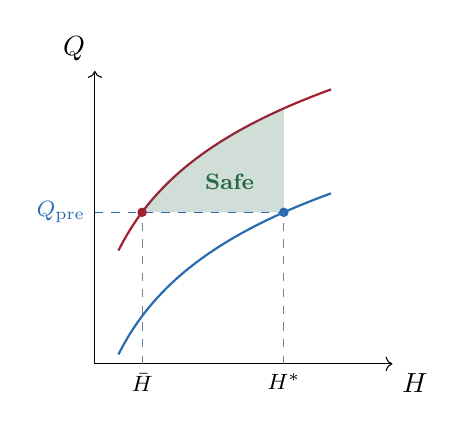
\begin{tikzpicture}[scale=0.60]
    \draw[->] (0,0) -- (6.3,0) node[below right] {$H$};
    \draw[->] (0,0) -- (0,6.2) node[above left] {$Q$};
    \draw[thick,ocean,domain=0.5:5,samples=100] plot (\x, {2.0*ln(\x+0.5)+0.2});
    \draw[thick,mitcardinal,domain=0.5:5,samples=100] plot (\x, {2.0*ln(\x+0.5)+2.4});
    \fill[forest,opacity=0.22] (1.0,3.208) -- plot[domain=1.0:4,samples=60] (\x, {2.0*ln(\x+0.5)+2.4}) -- (4,3.208) -- cycle;
    \filldraw[ocean] (4,3.208) circle (2.5pt);
    \draw[dashed,ocean] (0,3.208) -- (4,3.208);
    \node[left,font=\footnotesize,ocean] at (0,3.208) {$Q_{\text{pre}}$};
    \node[below,font=\footnotesize] at (4,0) {$H^*$};
    \draw[dashed,warmgray] (4,0) -- (4,3.208);
    \draw[dashed,warmgray] (1.0,0) -- (1.0,3.208);
    \node[below,font=\footnotesize] at (1.0,0) {$\bar{H}$};
    \filldraw[mitcardinal] (1.0,3.208) circle (2.5pt);
    \node[forest,font=\footnotesize\bfseries] at (2.85,3.85) {Safe};
\end{tikzpicture}
\end{column}
\begin{column}{0.45\textwidth}
\textbf{Cut hours, stay in the green.}
\vspace{0.3cm}

As long as you keep enough engagement, output is still up.
\vspace{0.3cm}

\textcolor{warmgray}{\small Some slack is fine. The curve rose enough to absorb it.}
\end{column}
\end{columns}
\end{frame}

\begin{frame}{Case III: cut too far, and you deskill}
\vspace{-0.5cm}
\begin{columns}
\begin{column}{0.55\textwidth}
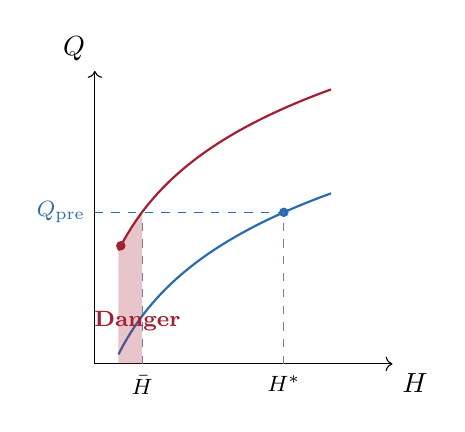
\begin{tikzpicture}[scale=0.60]
    \draw[->] (0,0) -- (6.3,0) node[below right] {$H$};
    \draw[->] (0,0) -- (0,6.2) node[above left] {$Q$};
    \draw[thick,ocean,domain=0.5:5,samples=100] plot (\x, {2.0*ln(\x+0.5)+0.2});
    \draw[thick,mitcardinal,domain=0.5:5,samples=100] plot (\x, {2.0*ln(\x+0.5)+2.4});
    \fill[mitcardinal,opacity=0.26] (0.5,0) -- plot[domain=0.5:1.0,samples=50] (\x, {2.0*ln(\x+0.5)+2.4}) -- (1.0,0) -- cycle;
    \filldraw[ocean] (4,3.208) circle (2.5pt);
    \draw[dashed,ocean] (0,3.208) -- (4,3.208);
    \node[left,font=\footnotesize,ocean] at (0,3.208) {$Q_{\text{pre}}$};
    \node[below,font=\footnotesize] at (4,-0.05) {$H^*$};
    \draw[dashed,warmgray] (4,0) -- (4,3.208);
    \node[below,font=\footnotesize] at (1.0,-0.05) {$\bar{H}$};
    \draw[dashed,warmgray] (1.0,0) -- (1.0,3.208);
    \filldraw[mitcardinal] (0.55,2.50) circle (2.5pt);
    \node[mitcardinal,font=\footnotesize\bfseries] at (0.9,0.9) {Danger};
\end{tikzpicture}
\end{column}
\begin{column}{0.45\textwidth}
\textbf{The red zone.} Skills fade, and you fall below where you started.
\vspace{0.3cm}

\textcolor{mitcardinal}{$\bullet$ Worse off than before AI.}
\vspace{0.3cm}

\lead{The point isn't to refuse the time savings. It's to be deliberate about them.}
\end{column}
\end{columns}
\end{frame}


% ---- time-use link: demand curve ----

\begin{frame}{Deskilling is real, but not deterministic}

The gains are real. People will use them.

\vspace{0.2cm}

The risk is also real: if agents let us bypass attention, we may stop building the human capital needed to judge the output.

\vspace{0.2cm}

\begin{center}
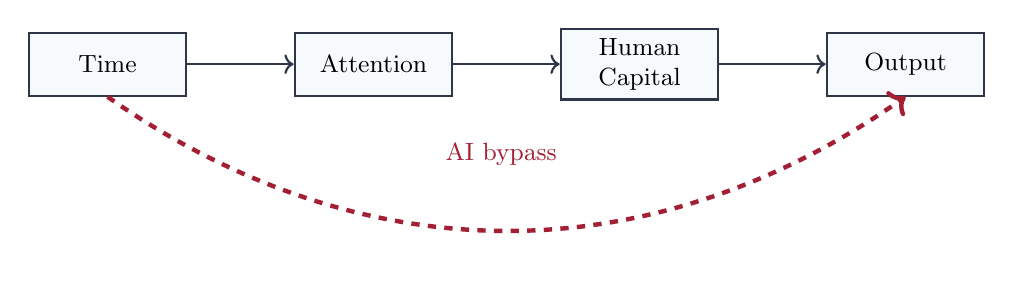
\begin{tikzpicture}[
    node distance=1.35cm,
    box/.style={rectangle, draw=charcoal, thick, fill=lightbg,
                minimum width=2.0cm, minimum height=0.8cm, align=center, font=\small}
]
    \node[box] (time) {Time};
    \node[box, right=of time] (attention) {Attention};
    \node[box, right=of attention] (hc) {Human\\Capital};
    \node[box, right=of hc] (output) {Output};

    \draw[->,thick,charcoal] (time) -- (attention);
    \draw[->,thick,charcoal] (attention) -- (hc);
    \draw[->,thick,charcoal] (hc) -- (output);

    \draw[->,ultra thick,mitcardinal,dashed] (time.south) to[bend right=35] (output.south);
    \node[mitcardinal,font=\small] at (5.0,-1.15) {AI bypass};
\end{tikzpicture}
\end{center}

\vspace{0.1cm}

\alert{This is a design problem, not destiny. Build verification workflows that keep judgment in the loop.}

\end{frame}




\begin{frame}{Trust Nothing and Verify Everything}

In April 2026, Sullivan \& Cromwell apologized to a federal judge after a filing contained AI-generated errors, including fabricated legal citations.

\vspace{0.35cm}

The striking part is that the firm's AI training already included the rule:

\vspace{0.35cm}

\begin{center}
{\Huge \textbf{Trust Nothing}}\\[0.2cm]
{\Huge \textbf{Verify Everything}}
\end{center}

\vspace{0.3cm}

\alert{AImost as if AI causes even experts to fall asleep at the wheel.}

\end{frame}


% =============================================================================
\section{Supply side of LLMs}
% =============================================================================

% ======================= TAMU NEW: how the machine works =======================
% Narrative (2026-10-01): history -> the machine (tokens, attention, next token, logit, weights) ->
% what it runs on (GPUs, NVIDIA, data centers) -> how you buy it -> (MIT) agents.

\begin{frame}{The transformer arrived in 2017, and everything followed}

\begin{center}
\footnotesize
\begin{tabular}{@{}ll@{}}
\toprule
\textbf{2013} & word2vec: words become vectors (Mikolov et al., Google) \\
\textbf{2014} & Attention is invented for machine translation (Bahdanau, Cho, Bengio) \\
\textbf{2017} & \textcolor{mitcardinal}{\textbf{``Attention Is All You Need'' introduces the transformer (Vaswani et al., Google)}} \\
\textbf{2018} & GPT-1 (OpenAI) and BERT (Google) \\
\textbf{2019} & GPT-2 \\
\textbf{2020} & GPT-3 \\
\textbf{Nov.\ 2022} & ChatGPT \\
\bottomrule
\end{tabular}
\end{center}

\vspace{0.4cm}

Earlier models read a sentence one word at a time and forgot the beginning by the end.

\vspace{0.25cm}

\alert{The transformer reads the whole passage at once, which is also what made it possible to train on GPUs in parallel.}

\end{frame}

\begin{frame}{OpenAI began as a nonprofit and is now valued above \$850 billion}

\begin{center}
\footnotesize
\begin{tabular}{@{}ll@{}}
\toprule
\textbf{Dec.\ 2015} & Founded as a nonprofit by Sam Altman, Elon Musk, and others \\
\textbf{2019} & Adds a capped-profit arm, and Microsoft invests \$1 billion \\
\textbf{Nov.\ 2022} & ChatGPT \\
\textbf{Nov.\ 2023} & The board fires Altman, and he is back within days \\
\textbf{Oct.\ 2025} & Becomes a public benefit corporation, with Microsoft holding about 27\% \\
\textbf{Mar.\ 2026} & Raises \$122 billion at an \$852 billion valuation \\
\textbf{June 2026} & Reported to file confidentially for an IPO \\
\bottomrule
\end{tabular}
\end{center}

\vspace{0.3cm}

In 2025 it reported revenue of \$13.1 billion and a net loss of \$38.5 billion.

\vspace{0.25cm}

\alert{Altman on the IPO, September 2026: ``I would say not 2026.''}

\vspace{0.1cm}
{\scriptsize\color{warmgray}Sources: CNBC and TechCrunch, March 2026; Bloomberg, August 2026; Fortune, September 12, 2026.}

\end{frame}

\begin{frame}{Anthropic left OpenAI over safety and is now heading to an IPO}

\begin{center}
\footnotesize
\begin{tabular}{@{}ll@{}}
\toprule
\textbf{2021} & Founded by former OpenAI researchers, led by Dario and Daniela Amodei \\
\textbf{Mar.\ 2023} & Claude 1 \\
\textbf{2023--2026} & Amazon and Google become its largest backers \\
\textbf{Feb.\ 2025} & Claude Code is released to the public \\
\textbf{Sept.\ 2025} & Valued at \$183 billion \\
\textbf{Feb.\ 2026} & Valued at \$380 billion \\
\textbf{May 2026} & Raises \$65 billion at a \$965 billion valuation \\
\textbf{June 2026} & Reported to file confidentially for an IPO \\
\bottomrule
\end{tabular}
\end{center}

\vspace{0.3cm}

Its 2025 revenue was about \$4.6 billion, and its annual run-rate passed \$47 billion by May 2026.

\vspace{0.25cm}

\alert{Reported this week: a listing as early as mid-November, at a valuation near \$2 trillion.}

\vspace{0.1cm}
{\scriptsize\color{warmgray}Sources: Anthropic, May 28, 2026; prospectus as reported by Reuters, September 28, 2026; Bloomberg, October 1, 2026.}

\end{frame}

% ---- the machine: stay with the transformer ----

\begin{frame}{The transformer is the engine inside every modern LLM}

\begin{center}
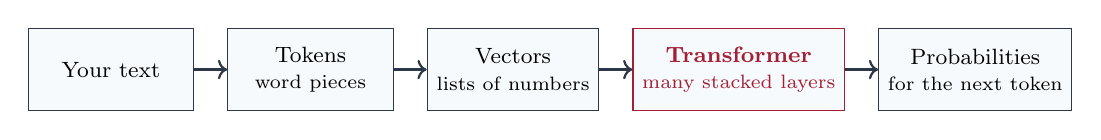
\begin{tikzpicture}[
  node distance=0.42cm,
  stage/.style={rectangle, draw=charcoal, fill=lightbg, minimum width=2.1cm, minimum height=1.05cm, align=center, font=\footnotesize},
]
\node[stage] (a) {Your text};
\node[stage, right=of a] (b) {Tokens\\\scriptsize{word pieces}};
\node[stage, right=of b] (c) {Vectors\\\scriptsize{lists of numbers}};
\node[stage, right=of c, draw=mitcardinal, text=mitcardinal] (d) {\textbf{Transformer}\\\scriptsize{many stacked layers}};
\node[stage, right=of d] (e) {Probabilities\\\scriptsize{for the next token}};
\draw[->,thick,charcoal] (a) -- (b);
\draw[->,thick,charcoal] (b) -- (c);
\draw[->,thick,charcoal] (c) -- (d);
\draw[->,thick,charcoal] (d) -- (e);
\end{tikzpicture}
\end{center}

\vspace{0.5cm}

\begin{itemize}\setlength\itemsep{0.3em}
    \item Text is chopped into tokens, and each token becomes a vector of numbers.
    \item Each layer rewrites every vector using the vectors around it.
    \item After dozens of layers, the last vector is turned into a probability for every possible next token.
\end{itemize}

\vspace{0.3cm}

\alert{Everything else in this talk --- chatbots, agents, Claude Code --- sits on top of this one machine.}

\end{frame}

\begin{frame}{The model reads tokens, not words}

\begin{center}
{\large Difference-in-differences estimates the treatment effect.}

\vspace{0.35cm}

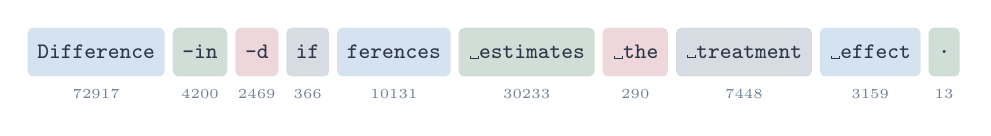
\begin{tikzpicture}[
  chip/.style={rectangle, rounded corners=2pt, inner xsep=3.5pt, inner ysep=4pt, font=\ttfamily\footnotesize, text=charcoal, minimum height=0.62cm},
  tokid/.style={font=\tiny, text=warmgray},
  node distance=2.5pt]
\node[chip, fill=ocean!20] (t1) {Difference};
\node[chip, fill=forest!22, right=of t1] (t2) {-in};
\node[chip, fill=mitcardinal!18, right=of t2] (t3) {-d};
\node[chip, fill=warmgray!28, right=of t3] (t4) {if};
\node[chip, fill=ocean!20, right=of t4] (t5) {ferences};
\node[chip, fill=forest!22, right=of t5] (t6) {\textvisiblespace estimates};
\node[chip, fill=mitcardinal!18, right=of t6] (t7) {\textvisiblespace the};
\node[chip, fill=warmgray!28, right=of t7] (t8) {\textvisiblespace treatment};
\node[chip, fill=ocean!20, right=of t8] (t9) {\textvisiblespace effect};
\node[chip, fill=forest!22, right=of t9] (t10) {.};
\node[tokid, below=1pt of t1] {72917};
\node[tokid, below=1pt of t2] {4200};
\node[tokid, below=1pt of t3] {2469};
\node[tokid, below=1pt of t4] {366};
\node[tokid, below=1pt of t5] {10131};
\node[tokid, below=1pt of t6] {30233};
\node[tokid, below=1pt of t7] {290};
\node[tokid, below=1pt of t8] {7448};
\node[tokid, below=1pt of t9] {3159};
\node[tokid, below=1pt of t10] {13};
\end{tikzpicture}
\end{center}

\vspace{0.25cm}

\begin{itemize}\setlength\itemsep{0.25em}
    \item This sentence becomes ten tokens, and each token has an ID number.
    \item Common words are one token, and rare words are split into pieces.
    \item GPT-4o's vocabulary has 200,019 tokens.
\end{itemize}

\vspace{0.2cm}

\alert{The model never sees letters or words. It sees this list of ten integers.}

\vspace{0.05cm}
{\scriptsize\color{warmgray}Real output from OpenAI's \texttt{o200k\_base} tokenizer, the one GPT-4o uses.}

\end{frame}

\begin{frame}{The vocabulary is a fixed list, decided before training begins}

\begin{center}
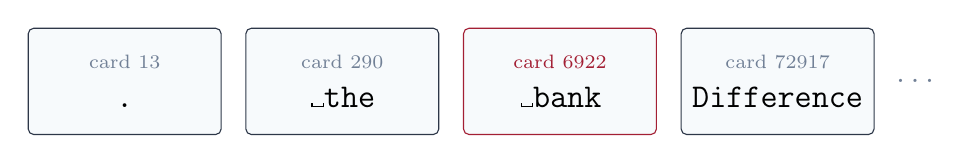
\begin{tikzpicture}[
  card/.style={rectangle, draw=charcoal, fill=lightbg, rounded corners=2pt, minimum width=2.45cm, minimum height=1.35cm, align=center},
  node distance=0.3cm]
\node[card] (c1) {{\scriptsize\color{warmgray}card 13}\\[2pt]{\ttfamily\large .}};
\node[card, right=of c1] (c2) {{\scriptsize\color{warmgray}card 290}\\[2pt]{\ttfamily\large \textvisiblespace the}};
\node[card, right=of c2, draw=mitcardinal] (c3) {{\scriptsize\color{mitcardinal}card 6922}\\[2pt]{\ttfamily\large \textvisiblespace bank}};
\node[card, right=of c3] (c4) {{\scriptsize\color{warmgray}card 72917}\\[2pt]{\ttfamily\large Difference}};
\node[font=\large, text=warmgray, right=0.15cm of c4] {\ldots};
\end{tikzpicture}
\end{center}

\vspace{0.3cm}

\begin{itemize}\setlength\itemsep{0.3em}
    \item Picture 200,019 flashcards in a fixed order, with one piece of text on each.
    \item The tokenizer swaps each piece of your sentence for its card number.
    \item The deck was settled before training started, and it never changes afterward.
    \item The number is a label, like a FIPS code. Card 6922 is not ``bigger'' than card 290.
\end{itemize}

\vspace{0.25cm}

\alert{The vocabulary is exogenous to you and to the model. Somebody fixed it in advance.}

\end{frame}

\begin{frame}{An algorithm built the list, and engineers chose its rules}

Nobody wrote the 200,019 cards by hand.

\vspace{0.1cm}

\begin{itemize}\setlength\itemsep{0.15em}
    \item The method is called byte-pair encoding.
    \item It starts with single characters and counts which neighboring pair appears most often in a very large body of text.
    \item It glues that pair into one new piece, then counts again, and repeats until the list reaches the chosen size.
    \item Frequent strings end up as one card, and rare strings are left in pieces.
\end{itemize}

\vspace{0.05cm}

The people involved are a small number of engineers at the lab. They pick the method, the text it counts, and how long the list should be.

\vspace{0.05cm}

\alert{That is why ``the'' is one card and ``differences'' is three: one is common in the text they counted, and the other is not.}

\vspace{0.05cm}
{\scriptsize\color{warmgray}Sennrich, Haddow, and Birch (2016) brought byte-pair encoding to language models.}

\end{frame}

\begin{frame}{Each card number looks up a vector, and the vector carries the meaning}

\begin{center}
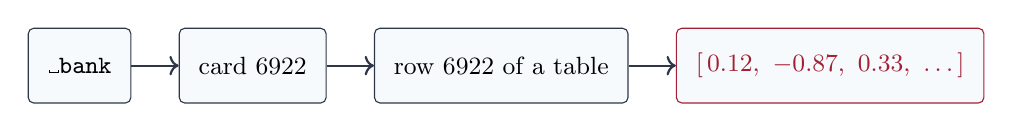
\begin{tikzpicture}[
  box/.style={rectangle, draw=charcoal, fill=lightbg, rounded corners=2pt, minimum height=0.95cm, align=center, font=\small, inner xsep=7pt},
  node distance=0.6cm]
\node[box] (a) {\ttfamily \textvisiblespace bank};
\node[box, right=of a] (b) {card 6922};
\node[box, right=of b] (c) {row 6922 of a table};
\node[box, right=of c, draw=mitcardinal, text=mitcardinal] (d) {$[\,0.12,\ -0.87,\ 0.33,\ \ldots\,]$};
\draw[->,thick,charcoal] (a) -- (b);
\draw[->,thick,charcoal] (b) -- (c);
\draw[->,thick,charcoal] (c) -- (d);
\end{tikzpicture}

\vspace{0.05cm}
{\scriptsize\color{warmgray}The numbers in the vector are illustrative.}
\end{center}

\vspace{0.05cm}

\begin{itemize}\setlength\itemsep{0.15em}
    \item The model keeps a table with one row for every card, and each row is thousands of numbers.
    \item Those rows are parameters, so they are estimated in training.
    \item The same card always starts from the same row, in every sentence.
\end{itemize}

\vspace{0.1cm}

\textbf{In our language:} the card number is a categorical variable, and its row is a fixed effect with thousands of dimensions.

\vspace{0.1cm}

\alert{The list of cards is chosen. What each card means is learned.}

\end{frame}






\begin{frame}{Attention lets every token look at the tokens before it}

\begin{center}
{\large She deposited the check at the \textcolor{mitcardinal}{\textbf{bank}}. \qquad We sat on the river \textcolor{mitcardinal}{\textbf{bank}}.}
\end{center}

\vspace{0.3cm}

Both sentences hand the model the same token, number 6922. It needs a different meaning in each.

\vspace{0.25cm}

\begin{itemize}\setlength\itemsep{0.3em}
    \item For each token, the model scores how relevant every earlier token is.
    \item Those scores become \textbf{attention shares} that sum to one.
    \item The token's new vector is a weighted average of the others, using those shares.
\end{itemize}

\vspace{0.25cm}

\textbf{In our language:} a kernel-weighted average, where the kernel is learned from data.

\vspace{0.25cm}

\alert{``Deposited'' and ``check'' pull \emph{bank} toward finance. ``River'' pulls it toward water.}

\end{frame}

\begin{frame}{Each token divides its attention among the tokens before it}

\begin{columns}[T]
\begin{column}{0.48\textwidth}
\centering
\textbf{Updating ``bank'' in sentence one}

\vspace{0.15cm}
{\footnotesize
\begin{tabular}{@{}lr@{}}
\toprule
Token & Share \\
\midrule
She & 0.04 \\
\textcolor{mitcardinal}{deposited} & \textcolor{mitcardinal}{0.38} \\
the & 0.03 \\
\textcolor{mitcardinal}{check} & \textcolor{mitcardinal}{0.33} \\
at & 0.05 \\
the & 0.03 \\
bank & 0.14 \\
\midrule
Total & 1.00 \\
\bottomrule
\end{tabular}}
\end{column}
\begin{column}{0.48\textwidth}
\centering
\textbf{Updating ``bank'' in sentence two}

\vspace{0.15cm}
{\footnotesize
\begin{tabular}{@{}lr@{}}
\toprule
Token & Share \\
\midrule
We & 0.05 \\
sat & 0.12 \\
on & 0.08 \\
the & 0.04 \\
\textcolor{mitcardinal}{river} & \textcolor{mitcardinal}{0.55} \\
bank & 0.16 \\
\midrule
Total & 1.00 \\
\bottomrule
\end{tabular}}
\end{column}
\end{columns}

\vspace{0.05cm}

\begin{center}
\alert{There is one such column for every token, in every layer. Each column sums to one on its own.}

\vspace{0.05cm}
{\scriptsize\color{warmgray}Illustrative shares, not model output.}
\end{center}

\end{frame}

\begin{frame}{Attention shares are computed from the text, not estimated}

For token $i$ looking at an earlier token $j$, with $x_i$ and $x_j$ their current vectors:

\vspace{-0.1cm}
\[
\text{score}_{ij} = (W_Q\, x_i)'(W_K\, x_j)
\qquad
a_{ij} = \frac{\exp(\text{score}_{ij})}{\sum_{k \le i}\exp(\text{score}_{ik})}
\qquad
x_i^{\text{new}} = \sum_{j \le i} a_{ij}\, W_V\, x_j
\]

\begin{itemize}\setlength\itemsep{0.3em}
    \item $W_Q$, $W_K$, and $W_V$ are parameters. They were estimated once, in training, and never change afterward.
    \item The shares $a_{ij}$ are not parameters. The model recomputes them for every new piece of text.
    \item They are applied to the other tokens' vectors, to mix their information into token $i$.
\end{itemize}

\vspace{0.3cm}

\alert{Nobody optimizes the shares directly. Training optimizes the matrices, and the shares fall out of the matrices and your text.}

\end{frame}

\begin{frame}{What an attention share can and cannot be}

\begin{center}
\footnotesize
\begin{tabular}{@{}ll@{}}
\toprule
Can it be negative? & No. It is a ratio of exponentials. \\
Can it be zero? & Only for later tokens, which are masked. Otherwise tiny but positive. \\
Can it exceed one? & No. The shares are positive and sum to one. \\
Why do they sum to one? & By construction, so that the update is a weighted average. \\
Is it a probability? & It has the same shape, but nothing is ever drawn from it. \\
Is it causal? & No. A large share does not mean that token caused the output. \\
\bottomrule
\end{tabular}
\end{center}

\vspace{0.3cm}

The formula for a share is the multinomial logit formula. The model uses it here to choose where to look, and again at the very end to choose the next token.

\vspace{0.25cm}

\alert{Same functional form, two different jobs. Only the last one is a prediction.}

\vspace{0.05cm}
{\scriptsize\color{warmgray}On causality: Jain and Wallace (2019), ``Attention is not Explanation.''}

\end{frame}

\begin{frame}{An LLM does one thing: it predicts the next token}

\begin{columns}[c]
\begin{column}{0.5\textwidth}
\begin{center}
{\large ``The minimum wage reduces \underline{\hspace{1.2cm}}''}
\end{center}
\end{column}
\begin{column}{0.46\textwidth}
\footnotesize
\begin{tabular}{@{}lr@{}}
\toprule
Next token & Probability \\
\midrule
employment & 0.41 \\
poverty & 0.22 \\
hours & 0.11 \\
inequality & 0.09 \\
\emph{every other token} & 0.17 \\
\bottomrule
\end{tabular}

\vspace{0.1cm}
{\scriptsize\color{warmgray}Illustrative numbers, not model output.}
\end{column}
\end{columns}

\vspace{0.45cm}

\begin{itemize}\setlength\itemsep{0.3em}
    \item The model draws one token from this distribution and appends it.
    \item Then it predicts again, with the longer text as the new input.
\end{itemize}

\vspace{0.3cm}

\alert{An essay, a proof, a Stata do-file: each is thousands of these draws in a row.}

\end{frame}

\begin{frame}{Next-token prediction is a multinomial logit}

\[
\Pr(\text{next token} = k \mid \text{context})
\;=\;
\frac{\exp\!\big(h(\text{context})' w_k\big)}{\sum_{j=1}^{V}\exp\!\big(h(\text{context})' w_j\big)}
\]

\vspace{0.2cm}

\begin{columns}[T]
\begin{column}{0.48\textwidth}
\textbf{What is familiar}
\begin{itemize}\setlength\itemsep{0.2em}
    \item The choice set is the vocabulary: $V$ is about 200,000 for GPT-4o.
    \item $w_k$ is the coefficient vector for alternative $k$.
    \item It is fit by maximum likelihood.
\end{itemize}
\end{column}
\begin{column}{0.48\textwidth}
\textbf{What is new}
\begin{itemize}\setlength\itemsep{0.2em}
    \item You do not choose the regressors.
    \item $h(\cdot)$ is the transformer, and it is learned jointly with $w$.
    \item There are billions of parameters, not a dozen.
\end{itemize}
\end{column}
\end{columns}

\vspace{0.35cm}

\alert{It is a prediction model. Nothing in the likelihood rewards being true, only being likely.}

\end{frame}

% ---- TAMU NEW (2026-10-02): vocabulary size vs the big numbers ----
\begin{frame}{200,000 is the number of choices, not the size of the model}
\vspace{0.1cm}
\begin{center}
\small
\renewcommand{\arraystretch}{1.25}
\begin{tabular}{@{}llrr@{}}
\toprule
 & \textbf{What it counts} & \textbf{GPT-3 (2020)} & \textbf{GPT-4o (2024)} \\
\midrule
\textcolor{mitcardinal}{\textbf{Vocabulary}} & distinct tokens it can choose from & 50,257 & 200,019 \\
Context window & tokens it can hold at once & 2,048 & 128,000 \\
Parameters & weights estimated in training & 175 billion & not disclosed \\
Training text & tokens it read during training & about 300 billion & not disclosed \\
\bottomrule
\end{tabular}
\end{center}
\vspace{0.2cm}

A dictionary has a few hundred thousand entries, and every book is written from them.
\vspace{0.2cm}

\alert{The choice set is small. What is enormous is the text it learned from and the weights it takes to choose well.}

\vspace{0.05cm}
{\scriptsize\color{warmgray}Sources: Brown et al.\ (2020) for GPT-3; OpenAI's \texttt{o200k\_base} tokenizer and model documentation for GPT-4o.}
\end{frame}

\begin{frame}{Vocabularies have grown, but only into the hundreds of thousands}
\begin{center}
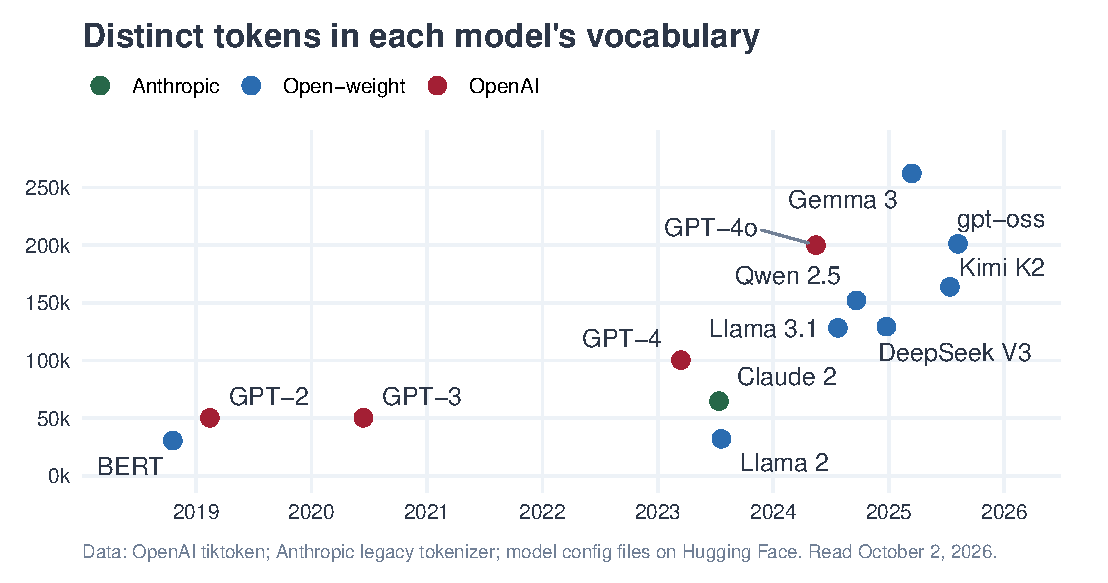
\includegraphics[width=\textwidth,height=0.72\textheight,keepaspectratio]{vocab_sizes.pdf}
\end{center}
\vspace{-0.3cm}
{\footnotesize\color{warmgray}Missing: Claude 3 and later, and other new closed models, which publish no tokenizer.}
\end{frame}

\begin{frame}{Training a model means estimating its weights}

\textbf{The weights} are the parameters of the model, $\theta$: the numbers inside every layer.

\vspace{0.15cm}

\begin{itemize}\setlength\itemsep{0.25em}
    \item Training shows the model real text and asks it to predict each next token.
    \item The weights are nudged, a little at a time, to make the true next token more likely.
\end{itemize}

\vspace{-0.1cm}
\[
\hat{\theta} \;=\; \arg\max_{\theta}\; \sum_{t} \log \Pr\nolimits_{\theta}\big(\text{token}_t \mid \text{tokens before } t\big)
\]

\textbf{In our language:} the objective is the log-likelihood of the true next token, summed over every position in the training text.

\vspace{0.15cm}

There is no closed form, so the maximum is found by stochastic gradient descent.

\vspace{0.2cm}

\alert{Once trained, the weights are fixed. When you chat with a model, nothing is being estimated; it is only being evaluated.}

\end{frame}

% ---- TAMU NEW (2026-10-02): one model, one objective ----
\begin{frame}{One model and one objective; the rest is computed along the way}
\vspace{0.1cm}
\begin{center}
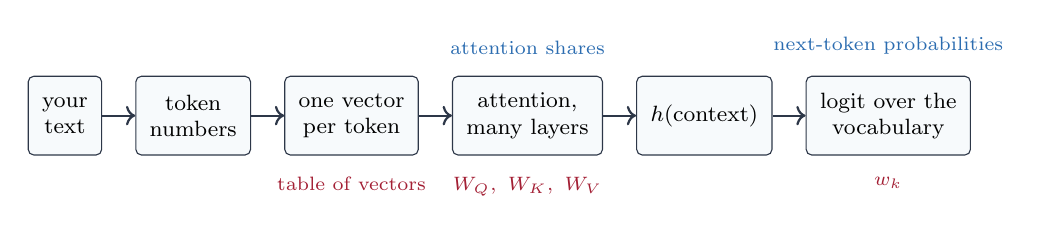
\begin{tikzpicture}[
  box/.style={rectangle, draw=charcoal, fill=lightbg, rounded corners=2pt, minimum height=1.0cm, align=center, font=\footnotesize, inner xsep=5pt},
  par/.style={font=\scriptsize, text=mitcardinal, align=center},
  comp/.style={font=\scriptsize, text=ocean, align=center},
  node distance=0.42cm]
\node[box] (a) {your\\text};
\node[box, right=of a] (b) {token\\numbers};
\node[box, right=of b] (c) {one vector\\per token};
\node[box, right=of c] (d) {attention,\\many layers};
\node[box, right=of d] (e) {$h(\text{context})$};
\node[box, right=of e] (f) {logit over the\\vocabulary};
\foreach \x/\y in {a/b,b/c,c/d,d/e,e/f} \draw[->,thick,charcoal] (\x) -- (\y);
\node[par, below=0.15cm of c] {table of vectors};
\node[par, below=0.15cm of d] {$W_Q,\ W_K,\ W_V$};
\node[par, below=0.15cm of f] {$w_k$};
\node[comp, above=0.15cm of d] {attention shares};
\node[comp, above=0.15cm of f] {next-token probabilities};
\end{tikzpicture}
\end{center}
\vspace{0.1cm}

\begin{itemize}\setlength\itemsep{0.35em}
    \item \textcolor{mitcardinal}{Red} is estimated: all the parameters are chosen together to maximize one likelihood.
    \item \textcolor{ocean}{Blue} is computed: the fixed parameters and your text go in, and these come out.
    \item Attention shares are a step inside $h(\cdot)$, and the probabilities are the final output.
\end{itemize}
\vspace{0.2cm}

\alert{There is no separate model for attention. Its matrices are estimated by the same next-token likelihood.}
\end{frame}

\begin{frame}{Three sets of numbers, and only one of them is ``the weights''}

\begin{center}
\scriptsize\setlength{\tabcolsep}{4pt}
\begin{tabular}{@{}llll@{}}
\toprule
 & \textbf{Parameters (``weights'')} & \textbf{Attention shares} & \textbf{Next-token probabilities} \\
\midrule
Where they come from & maximizing the likelihood & a logit formula inside $h(\cdot)$ & the logit formula at the end \\
What goes in & the training text & $W_Q$, $W_K$, and your text & $h(\text{context})$ and $w_k$ \\
When & once, before you use it & every layer, every token & once per token it writes \\
Fixed afterward? & yes & no & no \\
Can be negative? & yes & no & no \\
Sum to one? & no & yes, for each token & yes, over the vocabulary \\
Used for & every computation & mixing context into a token & drawing the next token \\
In the logit & the coefficients & part of $h(\text{context})$ & the fitted probabilities \\
\bottomrule
\end{tabular}
\end{center}

\vspace{0.3cm}

\alert{When someone says a model has 175 billion weights, they mean the first column. The other two are computed fresh each time.}

\end{frame}

% ---- what it runs on ----

\begin{frame}{Training also runs on hidden human labor}

Building the token list needed no human labelers, but training does.
\textbf{Mary L.\ Gray} of Microsoft Research, a 2020 MacArthur Fellow, and Siddharth Suri named this \emph{ghost work} in their 2019 book.

\vspace{0.1cm}

\begin{itemize}\setlength\itemsep{0.35em}
    \item People label text and images so that a model can learn from the labels.
    \item People read the worst material on the internet and flag it, so that a filter can learn to block it.
    \item People rate and correct a model's answers after it is trained, which is what makes it polite and useful.
\end{itemize}

\vspace{0.25cm}

\alert{In 2023 TIME reported that Kenyan workers labeling abusive text for OpenAI's filter took home less than \$2 an hour.}

\vspace{0.05cm}
{\scriptsize\color{warmgray}Sources: Gray and Suri, \emph{Ghost Work} (2019); Billy Perrigo, TIME, January 18, 2023.}

\end{frame}

\begin{frame}{GPUs do the arithmetic all at once}

\begin{columns}[T]
\begin{column}{0.48\textwidth}
\textbf{What the arithmetic is}
\begin{itemize}\setlength\itemsep{0.25em}
    \item Every layer is matrix multiplication.
    \item Billions of weights means billions of multiplications per token.
\end{itemize}
\end{column}
\begin{column}{0.48\textwidth}
\textbf{Why a GPU}
\begin{itemize}\setlength\itemsep{0.25em}
    \item A CPU has a few fast cores that work one step at a time.
    \item A GPU has thousands of simple cores that do the same operation in parallel.
\end{itemize}
\end{column}
\end{columns}

\vspace{0.45cm}

GPUs were built to draw video-game graphics, which is also a large pile of matrix arithmetic.

\vspace{0.35cm}

\alert{Training a frontier model ties up tens of thousands of GPUs for months, and every answer you receive runs on them too.}

\end{frame}

\begin{frame}{Inside a GPU: billions of switches doing one sum in parallel}

\begin{itemize}\setlength\itemsep{0.3em}
    \item A chip is a slab of silicon etched with billions of transistors, and each transistor is a switch that is on or off.
    \item Wire enough switches together and you get a circuit that multiplies two numbers and adds the result to a third.
    \item A CPU spends its switches on a few elaborate units that each do one complicated step after another.
    \item A GPU spends its switches on thousands of simple units that all do the same multiply-and-add at the same instant.
\end{itemize}

\vspace{0.2cm}

A matrix multiplication is millions of multiply-and-adds, and none of them has to wait for any other.

\vspace{0.2cm}

\alert{That is the whole match: the transformer is matrix multiplication, and the GPU is a machine for doing one sum a million times at once.}

\end{frame}

\begin{frame}{What limits a GPU is memory and heat}

\begin{columns}[T]
\begin{column}{0.48\textwidth}
\textbf{One NVIDIA H100}
\begin{itemize}\setlength\itemsep{0.25em}
    \item It holds 80 billion transistors.
    \item It has about 17,000 simple arithmetic cores, against 192 on a top server CPU.
    \item It carries 80 GB of memory beside the chip, because fetching the weights is slower than multiplying them.
\end{itemize}
\end{column}
\begin{column}{0.48\textwidth}
\textbf{The heat}
\begin{itemize}\setlength\itemsep{0.25em}
    \item One H100 draws up to 700 watts.
    \item Nearly all of that electricity leaves as heat.
    \item A rack of 72 newer GPUs draws roughly 120--130 kilowatts and is cooled with liquid.
\end{itemize}
\end{column}
\end{columns}

\vspace{0.35cm}

\alert{Put a few hundred thousand of these in one place and you have a data center measured in gigawatts.}

\vspace{0.1cm}
{\scriptsize\color{warmgray}Sources: NVIDIA product pages; DOE National Energy Technology Laboratory; HPE.}

\end{frame}

% ---- TAMU NEW (2026-10-01): GPU prices and training runs. Source notes: readings/gpu_prices_training.md ----
\begin{frame}{Each generation of GPU has cost more than the last}

\begin{center}
\footnotesize
\begin{tabular}{@{}llr@{}}
\toprule
\textbf{NVIDIA's top data-center GPU} & \textbf{Launched} & \textbf{Price of one chip} \\
\midrule
K80 & 2014 & \$5,000 \\
V100 & 2017 & about \$10,000 \\
A100 & 2020 & \$10,000--\$15,000 \\
H100 & 2023 & \$25,000--\$40,000 \\
Blackwell B200 & 2025 & \$30,000--\$40,000 \\
Blackwell Ultra B300 & late 2025 & \$38,000--\$49,000 \\
\bottomrule
\end{tabular}
\end{center}

\vspace{0.3cm}

\begin{itemize}\setlength\itemsep{0.3em}
    \item NVIDIA has not published a list price since 2014, so these are reported prices.
    \item Each chip also does far more: computation per dollar doubles about every two years.
\end{itemize}

\vspace{0.25cm}

\alert{The chip gets dearer and the arithmetic gets cheaper, both at once.}

\vspace{0.05cm}
{\scriptsize\color{warmgray}Sources: Epoch AI hardware data; Jensen Huang, CNBC, March 2024; HSBC via Epoch.}

\end{frame}

\begin{frame}{What each generation costs today}

\begin{center}
\footnotesize
\begin{tabular}{@{}llr@{}}
\toprule
\textbf{GPU} & \textbf{New in} & \textbf{Rent for one hour, October 2026} \\
\midrule
Blackwell Ultra GB300 & this year & from \$10.01 \\
Blackwell B200 & last year & \$6.25 \\
H200 & two years ago & \$4.38 \\
H100 & 2023 & \$3.40 \\
A100 & 2020 & \$1.82 \\
V100 & 2017 & \$0.97 \\
\bottomrule
\end{tabular}
\end{center}

\vspace{0.1cm}

\begin{itemize}\setlength\itemsep{0.15em}
    \item To buy: an H100 is about \$31,000 new and about \$19,000--\$23,000 used.
    \item An H100 rented for more than \$8 an hour in 2023 and about \$2 on resale markets by 2025.
\end{itemize}

\vspace{0.1cm}

\alert{How fast these chips lose value is the open accounting question behind the whole build-out.}

\vspace{0.05cm}
{\scriptsize\color{warmgray}Sources: getdeploying.com median on-demand prices; Silicon Data; Hashrate Index; CloudZero.}

\end{frame}

\begin{frame}{Training runs went from 10,000 GPUs to more than 100,000}

\begin{center}
\footnotesize
\begin{tabular}{@{}llll@{}}
\toprule
\textbf{Model} & \textbf{Year} & \textbf{GPUs used to train it} & \textbf{Estimated cost of the run} \\
\midrule
GPT-2 & 2019 & not disclosed & about \$4,000 \\
GPT-3 & 2020 & 10,000 V100s, for 15 days & \$2--\$4 million \\
GPT-4 & 2023 & not disclosed & \$40--\$78 million \\
Llama 3.1 (Meta) & 2024 & up to 16,000 H100s & \$53--\$170 million \\
Grok 4 (xAI) & 2025 & a 200,000-GPU cluster & about \$390 million \\
GPT-6 Astra & 2026 & more than 100,000 & \$0.5--\$1 billion \\
\bottomrule
\end{tabular}
\end{center}

\vspace{0.05cm}

\begin{itemize}\setlength\itemsep{0.1em}
    \item The low figure counts the hardware used up, and the high figure prices it at cloud rental rates.
\end{itemize}

\vspace{0.1cm}

\alert{The cost of the largest run grows about 2.4 times a year, and most labs do not say what they used.}

\vspace{0.05cm}
{\scriptsize\color{warmgray}Sources: Patterson et al.\ (2021); Meta; xAI; OpenAI briefing, September 2026; Epoch AI; Stanford AI Index; Cottier et al.\ (2024).}

\end{frame}

\begin{frame}{Anthropic reports its compute by company, not by model}

\textbf{What it has said, at the company level}
\begin{itemize}\setlength\itemsep{0.3em}
    \item It uses more than one million of Amazon's Trainium2 chips to train and serve Claude.
    \item It has contracted for up to one million of Google's TPU chips.
    \item It also runs on NVIDIA GPUs, including a cluster of more than 220,000.
\end{itemize}

\vspace{0.15cm}

\textbf{The one cost figure on record}
\begin{itemize}\setlength\itemsep{0.3em}
    \item Dario Amodei said Claude 3.5 Sonnet cost ``a few \$10M's'' to train.
\end{itemize}

\vspace{0.15cm}

\alert{Much of Claude is trained on chips that are not NVIDIA's, which is one reason the GPU counts are not comparable across labs.}

\vspace{0.05cm}
{\scriptsize\color{warmgray}Sources: Anthropic announcements, October 2025 to May 2026; Amodei (2025), as cited by Epoch AI.}

\end{frame}


\begin{frame}{NVIDIA sells the GPUs, and its stock is up tenfold in five years}
\begin{center}
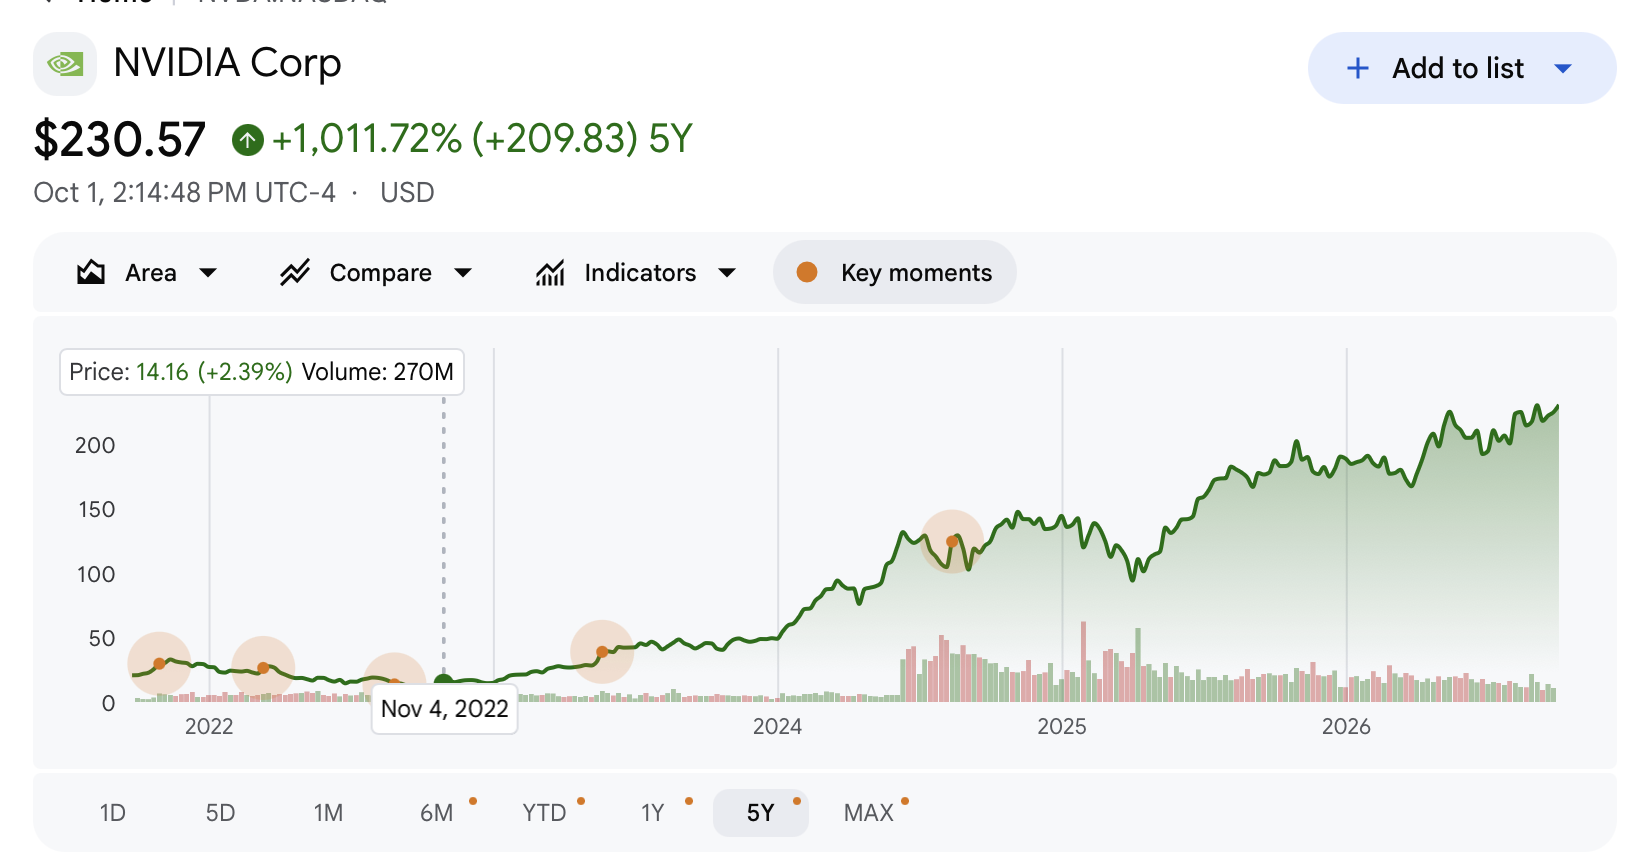
\includegraphics[width=0.86\textwidth,height=0.66\textheight,keepaspectratio]{nvidia_stock.png}
\end{center}
\vspace{-0.15cm}
\begin{center}{\color{warmgray}\scriptsize Source: Google Finance, October 1, 2026. Price \$230.57, up 1,012\% over five years.}\end{center}
\end{frame}

\begin{frame}{Compute is the scarce input, and it is rented by the hour}

\begin{columns}[T]
\begin{column}{0.5\textwidth}
\textbf{NVIDIA data-center revenue}

\vspace{0.1cm}
{\footnotesize
\begin{tabular}{@{}lr@{}}
\toprule
Fiscal 2022 & \$10.6 billion \\
Fiscal 2023 & \$15.0 billion \\
Fiscal 2024 & \$47.5 billion \\
Fiscal 2025 & \$115.2 billion \\
Fiscal 2026 & \$193.7 billion \\
\bottomrule
\end{tabular}}
\end{column}
\begin{column}{0.46\textwidth}
\textbf{What a GPU costs}
\begin{itemize}\setlength\itemsep{0.25em}
    \item One Blackwell chip sells for \$30,000--\$40,000.
    \item Renting one H100 costs about \$3.40 an hour.
    \item The final training run of GPT-4 cost \$40--\$80 million.
\end{itemize}
\end{column}
\end{columns}

\vspace{0.35cm}

\alert{The five largest cloud companies will spend more than \$690 billion on this in fiscal 2026.}

\vspace{0.1cm}
{\scriptsize\color{warmgray}Sources: NVIDIA annual results; Jensen Huang, CNBC, March 2024; getdeploying.com median, October 2026; Epoch AI and Stanford AI Index; FactSet, July 2026.}

\end{frame}

\begin{frame}{Data centers now show up in the national statistics}

\begin{itemize}\setlength\itemsep{0.3em}
    \item Data centers used 4.4\% of U.S.\ electricity in 2023, and the projection for 2028 is 6.7\% to 12\%.
    \item The five largest cloud companies will spend more than \$690 billion on capital in fiscal 2026.
    \item Debt paid for 32\% of that spending by mid-2026, up from 9\% two years earlier.
    \item Private office construction, the category that holds data centers, was up 30\% over the year in August 2026, while manufacturing construction was down 20\%.
    \item OpenAI's site in Abilene, Texas is planned for 1.2 gigawatts.
\end{itemize}

\vspace{0.2cm}

\alert{This is the largest private investment boom in the country, and it is concentrated in a handful of firms.}

\vspace{0.1cm}
{\scriptsize\color{warmgray}Sources: Lawrence Berkeley National Laboratory, 2024; FactSet, July 2026; Census Bureau, October 1, 2026; Epoch AI.}

\end{frame}

\begin{frame}{How much of GDP growth is AI? It depends on how you count}

\begin{center}
\footnotesize
\begin{tabular}{@{}lll@{}}
\toprule
\textbf{Who} & \textbf{Share of U.S.\ GDP growth} & \textbf{Period} \\
\midrule
Jason Furman & 92\% & first half of 2025 \\
St.\ Louis Fed & 39\% & first three quarters of 2025 \\
ING & about one third & second quarter of 2026 \\
Goldman Sachs & ``basically zero'' & 2025 \\
\bottomrule
\end{tabular}
\end{center}

\vspace{0.3cm}

\begin{itemize}\setlength\itemsep{0.3em}
    \item The high numbers count all spending on computers and software.
    \item The low numbers subtract imports, because most of the chips are made abroad.
\end{itemize}

\vspace{0.3cm}

\alert{The spending is enormous either way. How much of it is American output is a measurement question.}

\vspace{0.1cm}
{\scriptsize\color{warmgray}Sources: Furman, September 2025; Rubinton and Patro, St.\ Louis Fed, January 2026; Knightley, ING, August 2026; Hatzius, Goldman Sachs, 2026.}

\end{frame}

\begin{frame}{A majority in both parties opposes a data center nearby}

\begin{center}
\footnotesize
\begin{tabular}{@{}lcccc@{}}
\toprule
\textbf{Percent opposed} & \textbf{All} & \textbf{Democrats} & \textbf{Independents} & \textbf{Republicans} \\
\midrule
NBC News, August--September 2026 & 69 & 81 & 71 & 57 \\
Heatmap, May 2026 & 71 & 78 & 72 & 63 \\
UMass Amherst, August 2026 & 65 & 76 & 67 & 52 \\
\bottomrule
\end{tabular}
\end{center}

\vspace{0.2cm}

\begin{itemize}\setlength\itemsep{0.2em}
    \item One year earlier the country was split: 43\% in favor and 42\% opposed.
    \item Local opposition blocked or delayed \$64 billion of projects between May 2024 and March 2025.
    \item Of the officials publicly opposing projects, 55\% were Republicans and 45\% were Democrats.
\end{itemize}

\vspace{0.25cm}

\alert{Almost nothing else in American politics polls like this.}

\vspace{0.1cm}
{\scriptsize\color{warmgray}Sources: NBC News; Heatmap and Embold; UMass Amherst Poll; Data Center Watch.}

\end{frame}

\begin{frame}{The two parties object with different emphasis}

\begin{center}
\footnotesize
\begin{tabular}{@{}lcc@{}}
\toprule
\textbf{Percent who say data centers are\ldots} & \textbf{Democrats} & \textbf{Republicans} \\
\midrule
mostly bad for the environment & 62 & 47 \\
mostly bad for home energy costs & 58 & 44 \\
a worry for the local water supply & 67 & 49 \\
a benefit for technological advancement & 54 & 60 \\
\bottomrule
\end{tabular}
\end{center}

\vspace{0.15cm}

\begin{itemize}\setlength\itemsep{0.15em}
    \item Democratic officials stress the environment and the use of water and power.
    \item Republican officials stress tax incentives and strain on the grid.
    \item In November 2025 two Democrats won seats on Georgia's utility commission, the party's first since 2000, in a race about power bills.
\end{itemize}

\vspace{0.15cm}

\alert{The coalition against them is broad, and the industry that needs them is the one driving investment.}

\vspace{0.1cm}
{\scriptsize\color{warmgray}Sources: Pew Research Center, August 2026; AP-NORC and EPIC, July 2026; Data Center Watch.}

\end{frame}

% ---- how you buy it ----

\begin{frame}{Closed models lead, and open-weight models run on your own machine}

\begin{columns}[T]
\begin{column}{0.48\textwidth}
\textbf{Closed models} \\
\textcolor{warmgray}{\scriptsize Claude, GPT, Gemini}

\vspace{0.2cm}
\begin{itemize}\setlength\itemsep{0.2em}
    \item The weights are a trade secret.
    \item You rent them by subscription or by the token.
    \item Your text goes to their servers.
    \item They are the frontier.
\end{itemize}
\end{column}
\begin{column}{0.48\textwidth}
\textbf{Open-weight models} \\
\textcolor{warmgray}{\scriptsize Llama, Qwen, DeepSeek, Gemma, Mistral, gpt-oss}

\vspace{0.2cm}
\begin{itemize}\setlength\itemsep{0.2em}
    \item You download the weights.
    \item You run them with Ollama or LM Studio.
    \item Your data never leaves your machine.
    \item A 16--32 GB laptop runs a 20--30 billion parameter model.
\end{itemize}
\end{column}
\end{columns}

\vspace{0.35cm}

\alert{The best open-weight model scored 44 and the best closed model 53 on the same public index in September 2026. Private and free costs you about nine points.}

\vspace{0.1cm}
{\scriptsize\color{warmgray}Source: Artificial Analysis Intelligence Index, September 7, 2026.}

\end{frame}

\begin{frame}[fragile]{Effort is a dial for how hard the model thinks}

Before the answer you see, a model can write itself a private scratchpad of reasoning tokens.

\vspace{0.1cm}

\begin{center}
\footnotesize
\begin{tabular}{@{}lll@{}}
\toprule
 & \textbf{Claude} & \textbf{OpenAI} \\
\midrule
Name of the dial & \texttt{effort} & \texttt{reasoning\_effort} \\
Settings & low, medium, high, xhigh, max & minimal, low, medium, high, xhigh \\
In the coding agent & \texttt{/effort high} in Claude Code & set per model in Codex \\
\bottomrule
\end{tabular}
\end{center}

\vspace{0.1cm}

\begin{itemize}\setlength\itemsep{0.1em}
    \item Higher effort means more reasoning tokens, more tool calls, and longer answers.
    \item You pay for every one of those tokens, in dollars and in waiting time.
    \item Low effort is right for a rename, and high effort is right for a proof or a tricky merge.
\end{itemize}

\vspace{0.15cm}

\alert{Same model, same weights. Effort only changes how many tokens it spends before it commits.}

% Sources: Anthropic effort docs (platform.claude.com/docs/en/build-with-claude/effort); OpenAI reasoning guide. Checked 2026-10-01.

\end{frame}

\begin{frame}{You buy intelligence by the token or by the month}

\begin{columns}[T]
\begin{column}{0.56\textwidth}
\textbf{By the token (the API)}

\vspace{0.1cm}
{\footnotesize
\begin{tabular}{@{}lrr@{}}
\toprule
Dollars per million tokens & In & Out \\
\midrule
Claude Fable 5.1 & 10 & 50 \\
Claude Opus 5.5 & 4 & 20 \\
Claude Haiku 4.5 & 1 & 5 \\
GPT-6 Astra & 10 & 50 \\
GPT-6.1 Sol & 2 & 10 \\
GPT-6 Luna & 0.10 & 0.50 \\
\bottomrule
\end{tabular}}
\end{column}
\begin{column}{0.4\textwidth}
\textbf{By the month (a subscription)}
\begin{itemize}\setlength\itemsep{0.25em}
    \item Claude Pro is \$20.
    \item Claude Max is \$100 or \$200.
    \item Claude Code is included.
\end{itemize}

\vspace{0.2cm}
A million tokens is about 750,000 words.
\end{column}
\end{columns}

\vspace{0.3cm}

\alert{Use a subscription for your daily work. Use the API when a script must label 300,000 documents overnight.}

\vspace{0.1cm}
{\scriptsize\color{warmgray}Sources: Anthropic and OpenAI pricing pages, October 1, 2026.}

\end{frame}

% ===================== end TAMU NEW (MIT slides resume) =====================



% =============================================================================
% TAMU NEW (2026-10-02): The API and open weights (keys, credits, running your own model)
% SPEAKER DIRECTIONS (Scott) -- this is a SLOW-DOWN + LIVE DEMO moment:
%   - Most of the room has a subscription; few have made an API key. Normalize it:
%     it is just a billed password for your code. Do not assume they know what "API" means.
%   - Pre-stage the demo so wifi can't sink it:
%       (1) platform.kimi.ai open in a tab, logged in, balance visible, near "Create API Key"
%       (2) a terminal with Claude Code open in the running-example repo
%       (3) the key already in an env var OFF-SCREEN; never show the real key on the projector
%   - Demo beats: show the balance -> create a key -> hand Claude the env var ->
%     "run one Kimi agent on the example" -> open the transcript -> read the RAW reasoning trace.
%   - The punchline of the demo is the un-obfuscated trace, which closed models hide.
%   - Fallback if live fails: pre-captured screenshots (TODO: drop in misc/figures/). Keep moving; never debug live.
%   - Why-open-weights beats to say aloud: raw traces, permanent pinning (reproducibility),
%     cost, privacy, a second model family for external validity.
% =============================================================================

% ---- TAMU NEW (2026-10-02): transition divider into the agents section ----
\begin{frame}[plain]
\vfill
\begin{center}
{\LARGE\bfseries\textcolor{charcoal}{Introducing AI Agents}}\\[0.35cm]
{\large\textcolor{warmgray}{From tools you prompt to tools that act}}
\end{center}
\vfill
\end{frame}

\begin{frame}{Use agents when the work is valuable, slow, and checkable}

My view: delegate to agents when a task satisfies all four conditions.

\vspace{0.25cm}

\begin{enumerate}\setlength\itemsep{0.25em}
    \item \textbf{The output is highly valuable.} \\
    {\small\color{warmgray} The stakes justify the setup cost.}

    \item \textbf{The task is time-intensive for humans.} \\
    {\small\color{warmgray} Hours or days of skilled effort, not minutes.}

    \item \textbf{The probability humans do it well is low.} \\
    {\small\color{warmgray} Difficult to execute at high quality consistently.}

    \item \textbf{The output can be verified.} \\
    {\small\color{warmgray} You can inspect, compare, rerun, or source-ground it.}
\end{enumerate}

\vspace{0.25cm}
\alert{Coding is the canonical example, but this also describes literature review, replication, deck creation, and referee-style review.}

\end{frame}



\begin{frame}{Agents are different because they act}

A spectrum of AI use, from passive to autonomous:

\vspace{0.4cm}

\begin{center}
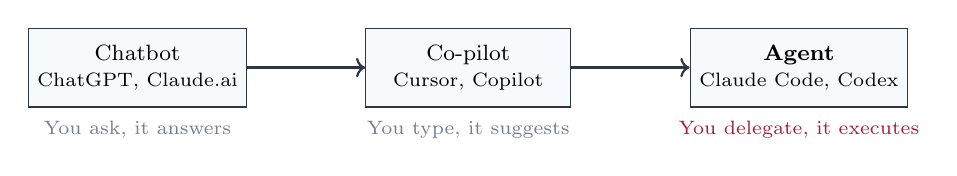
\begin{tikzpicture}[
  x=1.4cm, y=1cm,
  spectrumbox/.style={rectangle, draw=charcoal, fill=lightbg, minimum width=2.6cm, minimum height=1.0cm, align=center, font=\footnotesize},
]
\node[spectrumbox] (a) at (0, 0) {Chatbot\\\scriptsize{ChatGPT, Claude.ai}};
\node[spectrumbox] (b) at (3, 0) {Co-pilot\\\scriptsize{Cursor, Copilot}};
\node[spectrumbox] (c) at (6, 0) {\textbf{Agent}\\\scriptsize{Claude Code, Codex}};
\draw[->,thick,charcoal] (a) -- (b);
\draw[->,thick,charcoal] (b) -- (c);
\node[font=\scriptsize\color{warmgray}, below=0.05cm of a, align=center] {You ask, it answers};
\node[font=\scriptsize\color{warmgray}, below=0.05cm of b, align=center] {You type, it suggests};
\node[font=\scriptsize\color{mitcardinal}, below=0.05cm of c, align=center] {You delegate, it executes};
\end{tikzpicture}
\end{center}

\vspace{0.6cm}

\textbf{An agent} reads files, writes code, runs it, reads the output, and decides what to do next across many steps.

\end{frame}

\begin{frame}[fragile]{What the agent actually does}

An agent is not just a chatbot with better prose. It acts on your project.

\vspace{0.05cm}

\begin{center}
\scriptsize
\begin{tabular}{ll}
\toprule
\texttt{ls data/} & list files \\
\texttt{rg "minimum wage" .} & search text and code \\
\texttt{grep -r "treated" code/} & search inside files \\
\texttt{curl -O https://site.gov/data.csv} & download from the web \\
\texttt{Rscript estimate.R} & run an R script \\
\texttt{python audit.py} & run a Python script \\
\texttt{stata -b do analysis.do} & run a Stata do-file \\
\texttt{pdflatex paper.tex} & compile a paper or deck \\
\texttt{git diff} & inspect changes \\
\textcolor{mitcardinal}{\texttt{rm -rf data/}} & \textcolor{mitcardinal}{delete files, permanently} \\
\textcolor{mitcardinal}{\texttt{diskutil eraseDisk ...}} & \textcolor{mitcardinal}{format a hard drive} \\
\bottomrule
\end{tabular}
\end{center}

\vspace{0.05cm}

\alert{It reads files, writes files, runs commands, sees errors, revises, and tries again.}

\end{frame}

\begin{frame}{Reasoning models and agents are merging}

\begin{columns}[T]
\begin{column}{0.48\textwidth}
\textbf{Reasoning LLMs} \\
\textcolor{warmgray}{\scriptsize o1, o3, DeepSeek R1, Claude extended thinking}

\vspace{0.25cm}
\begin{itemize}\setlength\itemsep{0.15em}
    \item Trained to deliberate before answering
    \item Pure inference: no action in the world
    \item Strong at math, code, logic puzzles
\end{itemize}
\end{column}

\begin{column}{0.48\textwidth}
\textbf{AI agents} \\
\textcolor{warmgray}{\scriptsize ReAct, tool use, Claude Code, Cursor, Codex}

\vspace{0.25cm}
\begin{itemize}\setlength\itemsep{0.15em}
    \item LLM + tools: read, write, run, search
    \item Loop: act, observe, decide, repeat
    \item Strong at long, multi-step tasks
\end{itemize}
\end{column}
\end{columns}

\vspace{0.4cm}

\alert{2025--26: the merger.} Frontier systems increasingly \emph{think} and \emph{act}: plan a task, execute steps, check output, and revise.

\end{frame}

% ---- TAMU NEW (2026-10-02): reasoning traces. Sources: Anthropic and OpenAI API docs; TechCrunch 2026-02-23 ----
\begin{frame}{A reasoning agent leaves a trace, and the trace is data}

\textbf{What is in a trace}
\begin{itemize}\setlength\itemsep{0.25em}
    \item the reasoning the model wrote to itself before it acted
    \item every command it ran and every file it opened
    \item everything it saw come back, including the errors
\end{itemize}

\vspace{0.25cm}

\textbf{Why it matters to a researcher}
\begin{itemize}\setlength\itemsep{0.25em}
    \item Claude Code saves each session to a transcript file on your machine.
    \item A transcript is text, so an agent can read hundreds of them and code what happened.
    \item This is how I learned what my agents did that their finished output never showed.
\end{itemize}

\vspace{0.25cm}

\alert{The output tells you what the agent concluded. The trace tells you what it did to get there.}

\end{frame}

% ---- TAMU NEW (2026-10-02): a real Kimi trace excerpt from the minimum-wage runs ----
\begin{frame}{A trace from the minimum-wage runs (Kimi, open-weight)}

One agent's own account of the choices it made:

\vspace{0.35cm}

\begin{quote}
\small\itshape ``Post-2009 period chosen because the federal minimum wage was constant at \$7.25, creating clean cross-state variation. Callaway--Sant'Anna drops 15 states already treated in 2010 (no pre-treatment data in the sample). Effective sample: 36 states, 16 treated and 20 never-treated.''
\end{quote}

\vspace{0.35cm}

\alert{Every choice is in the trace: the window, the estimator, the dropped states. We extract these from every run.}

\end{frame}

\begin{frame}{Closed models summarize the reasoning; open ones show all of it}

\begin{center}
\footnotesize
\begin{tabular}{@{}ll@{}}
\toprule
\textbf{Model} & \textbf{What you get of its reasoning} \\
\midrule
Claude (Anthropic) & a summary of the thinking, not the raw text \\
GPT reasoning models (OpenAI) & hidden, with a summary on request \\
Kimi, DeepSeek, Qwen (open-weight) & the full raw reasoning \\
\bottomrule
\end{tabular}
\end{center}

\vspace{0.3cm}

\begin{itemize}\setlength\itemsep{0.25em}
    \item Closed labs summarize the raw reasoning, citing competitive advantage and keeping rivals from training on it.
    \item What the summary leaves out is unknown.
    \item You can raise the effort setting and get more, but you pay for that too.
\end{itemize}

\vspace{0.2cm}
{\scriptsize\color{warmgray}Sources: Anthropic and OpenAI developer documentation.}

\end{frame}

\begin{frame}{So I study both, and I want to close the gap}

\begin{itemize}\setlength\itemsep{0.35em}
    \item To study how agents behave I have needed all of the reasoning, so I run experiments on open and closed models alike.
    \item My running question: can a harness that follows a checklist I have been building make a cheaper model work like an expensive one?
    \item Kimi is cheaper, so I want to know whether harnessing it can close the gap.
\end{itemize}

\vspace{0.45cm}

\alert{To study that, I have needed the traces: the trace is how you see what the agent is actually doing.}

\end{frame}


\begin{frame}{Claude Code began as a terminal agent}

\textbf{Boris Cherny} joined Anthropic in 2024. Late that year he gave Claude direct access to his terminal and asked it to fix his Spotify playlists.

\vspace{0.3cm}

Claude wrote API calls, read its own output, handled errors, and finished the job autonomously. \textit{That was the proof-of-concept.}

\vspace{0.35cm}

\begin{itemize}\setlength\itemsep{0.15em}
    \item \textbf{Sept.\ 2024.} Cherny builds the prototype as a side project.
    \item \textbf{Nov.\ 2024.} Released inside Anthropic.
    \item \textbf{Feb.\ 24, 2025.} Public research preview with Claude 3.7 Sonnet.
    \item \textbf{May 2025.} General availability.
    \item \textbf{Nov.\ 25, 2025.} Claude Code lands inside the desktop app.
\end{itemize}

\vspace{0.25cm}

\alert{Desktop integration of Claude Code is to AI agents what ChatGPT was to GPT --- product, not capability, is probably the unspoken hero of this revolution.}
\end{frame}

\begin{frame}[shrink=4]{Install Claude Code by asking Claude to install it}

You have to get Claude Code onto your machine somehow. The install command is the first place phishing finds you.

\vspace{0.25cm}

\begin{columns}[T]
\begin{column}{0.47\textwidth}
\textbf{The trojan-horse problem}
\begin{itemize}\setlength\itemsep{0.1em}
    \item cloned sites imitating \texttt{claude.ai}, GitHub, package docs
    \item ``copy'' buttons that hide a different command than the one shown
    \item pasting an unfamiliar install command is voluntary malware
\end{itemize}
\end{column}
\begin{column}{0.47\textwidth}
\textbf{The defensive habit}
\begin{itemize}\setlength\itemsep{0.1em}
    \item open the desktop app (or another agent you trust)
    \item give it the URL you were about to paste from
    \item have it inspect domain, repo, command, and explain
    \item run nothing until the explanation matches what you expect
\end{itemize}
\end{column}
\end{columns}

\vspace{0.25cm}

\alert{Anthropic is currently doing better than most at not getting cloned. That will not last. Build the habit before the arms race catches up.}

\end{frame}

\begin{frame}[fragile]{Claude is not one interface}

The terminal is where Claude Code began. It is still the cleanest place to work with project folders, code, data, and reproducible files.

\vspace{0.25cm}

\begin{columns}[T]
\begin{column}{0.47\textwidth}
\textbf{CLI / terminal}
\begin{itemize}\setlength\itemsep{0.12em}
    \item Project directories
    \item File edits and code runs
    \item Repeatable workflows
\end{itemize}
\end{column}

\begin{column}{0.47\textwidth}
\textbf{Desktop / Cowork}
\begin{itemize}\setlength\itemsep{0.12em}
    \item Conversational work
    \item Shared context
    \item Faster collaboration loops
\end{itemize}
\end{column}
\end{columns}

\vspace{0.25cm}

\begin{verbatim}
Read Chris Cornwell's Claude academic guide:
https://cornwl.github.io/files/claude-academic-guide.html

Explain which parts apply to my project.
Help me choose CLI, Desktop/Cowork, or both.
\end{verbatim}

\end{frame}

\begin{frame}{Agents are a general-purpose technology}

The same agent runs my Callaway--Sant'Anna replication \emph{and} grabs a file off the internet when I need it.

\vspace{0.25cm}

\begin{columns}[T]
\begin{column}{0.47\textwidth}
\textbf{Trivial uses}
\begin{itemize}\setlength\itemsep{0.1em}
    \item push to my repos
    \item edit my website
    \item update my CV
    \item fetch from the internet
\end{itemize}
\end{column}
\begin{column}{0.47\textwidth}
\textbf{Sophisticated uses}
\begin{itemize}\setlength\itemsep{0.1em}
    \item replication audits
    \item bibliography checks
    \item package comparisons
    \item many-agent experiments
\end{itemize}
\end{column}
\end{columns}

\vspace{0.3cm}

\alert{Most of the daily learning about how to work with agents happens at the trivial end.}

\end{frame}

% ---- TAMU NEW (2026-10-02): desktop vs terminal, factual, Scott's own view ----
\begin{frame}{Desktop or terminal: pick what fits your brain}
Both run the same agent. The choice is about workflow, not capability.
\vspace{0.3cm}
\begin{columns}[T]
\begin{column}{0.48\textwidth}
\textbf{The desktop app (what I reach for)}
\begin{itemize}\setlength\itemsep{0.25em}
    \item The chatbot and the coding agents sit together, which suits a conversational, thinking-partner way of working.
    \item Folders, with sessions inside them, match how I organize my research.
    \item The tradeoff: it is slower.
\end{itemize}
\end{column}
\begin{column}{0.48\textwidth}
\textbf{The terminal (what I use for speed)}
\begin{itemize}\setlength\itemsep{0.25em}
    \item It is noticeably faster. I cannot fully explain why, but it is.
    \item The cost is window sprawl; tools like Ghostty help, and some prefer an IDE such as VS Code.
\end{itemize}
\end{column}
\end{columns}
\vspace{0.35cm}
\alert{I use both: the desktop app to think, the terminal when speed matters.}
\end{frame}

\begin{frame}{Three operating modes}

\footnotesize

\begin{center}
\renewcommand{\arraystretch}{1.4}
\begin{tabular}{@{}p{0.42\textwidth}p{0.34\textwidth}l@{}}
\toprule
\textbf{Mode} & \textbf{What it does} & \textbf{Where} \\
\midrule
\textbf{Plan} & Read-only. Searches, reads, proposes. No state changes. & CLI \& Desktop \\
\textbf{Action} & Edits, runs, writes. Each risky tool call requests approval. & CLI \& Desktop \\
\textbf{\texttt{--dangerously-skip-permissions}} & Edits, runs, writes --- no approvals. The agent runs free. & \textbf{CLI only} \\
\bottomrule
\end{tabular}
\end{center}

\vspace{0.25cm}

\textbf{Why the third mode matters:} the agent goes fast. Launch a long task, walk away, come back to a finished result. Not available in the desktop app. You have given up the per-tool checkpoint, so the safety question is no longer the flag --- it is the blast radius of the folder.

\end{frame}

% ---- TAMU NEW (2026-10-02): plan mode usage (Paul Goldsmith-Pinkham) + Scott's caveat ----
\begin{frame}{Plan mode: iterate on the design, not the files}
\textbf{Read-only:} the agent reads and proposes, but changes nothing until you approve.
\vspace{0.45cm}
\textbf{How Paul Goldsmith-Pinkham uses it:}
\begin{itemize}\setlength\itemsep{0.3em}
    \item Research the data, then let plan mode design the whole pipeline.
    \item It writes the plan to a file, so the design survives a fresh context.
    \item Only then execute, building from the plan.
\end{itemize}
\vspace{0.5cm}
\alert{Iterate on the design, which is cheap, before the code, which is not.}
\vspace{0.25cm}
{\small\color{warmgray}\textit{Confession: I jump in and try not to drown, so plan mode has never been my habit. If you're more deliberate than me, start here.}}
\end{frame}

% ---- TAMU NEW (2026-10-02): IDEs ----
\begin{frame}{IDEs: open a whole folder and see everything}
An IDE (integrated development environment) is a workspace built around your whole project, not one file at a time.
\vspace{0.3cm}
\begin{itemize}\setlength\itemsep{0.25em}
    \item You open a folder and see the entire codebase at once, with side panels for files, packages, and a terminal.
    \item When the agent edits files you watch it happen: changed files are flagged, and edited lines are marked right in the margin.
    \item Examples: VS Code (the common one), Kiro (agent-first), and Positron (Posit's data-science IDE, the RStudio successor).
\end{itemize}
\vspace{0.3cm}
\alert{The CLI is a message in a bottle: fast, but you cannot see the files. An IDE lets you watch the diffs as they land.}
\end{frame}

% =============================================================================
% TAMU NEW (2026-10-02): Code review + Claude in the loop (GitHub PR workflow)
% SPEAKER DIRECTIONS (Scott) -- LIVE DEMO:
%   - Do NOT name the firm; say "a large tech firm" (code.techfirm.dev, "cr"). Frame as what you have
%     learned the large firms do. Do not describe anything proprietary/NDA.
%   - Repo for the demo: ~/mixtape_harness (your GitHub repo scunning1975/mixtape_harness).
%   - Pre-stage so wifi can't sink it: `gh auth status` logged in; a branch + small change ready.
%   - Demo path: branch + small edit -> `gh pr create` -> open PR "Files changed" in browser ->
%     leave one inline comment -> in Claude Code: `gh pr view 42 --comments` then fix -> push -> refresh PR.
%   - Then show `/code-review 42 --comment` and `/loop 10m "..."` cycling live.
%   - SAY THE CAVEAT OUT LOUD: /loop is session-scoped (stops when the terminal closes); 24/7 = Routines or GitHub Actions.
% =============================================================================


% ---- transition divider: the API + open weights ----
\begin{frame}[plain]
\vfill
\begin{center}
{\LARGE\bfseries\textcolor{charcoal}{The API, and Models You Run Yourself}}\\[0.35cm]
{\large\textcolor{warmgray}{Keys, credits, and installing an open-weight model}}
\end{center}
\vfill
\end{frame}

% ---- what an API key is + why ----
\begin{frame}{An API key is a billed password for your code}
API stands for Application Programming Interface: a way for your code to call the model directly, with no app in between.
\vspace{0.35cm}
\begin{itemize}\setlength\itemsep{0.3em}
    \item The key is a secret string that authenticates you and charges the usage to your account.
    \item You reach for it when you script the model: many agents at once, an overnight job, or a model your subscription does not include.
\end{itemize}
\vspace{0.4cm}
\alert{A subscription is for you at the keyboard. The API is for your code, running on its own.}
\end{frame}

% ---- get a key + credits + URLs ----
\begin{frame}{Get a key, load credits, paste it in}
\begin{itemize}\setlength\itemsep{0.35em}
    \item The same three steps at each lab: create an account, add a card, generate a key.
    \item \textbf{OpenAI:} \texttt{platform.openai.com} \hfill \textbf{Anthropic:} \texttt{console.anthropic.com} \hfill \textbf{Kimi:} \texttt{platform.kimi.ai}
    \item Credits are pay-as-you-go: load a balance (say \$20) and each call draws it down.
    \item The key lives in an environment variable, never in your code and never on a slide.
\end{itemize}
\vspace{0.4cm}
\alert{Treat the key like a card number: it spends real money, so guard it and set a low cap.}
\end{frame}

% ---- open weights via Claude Code + why ----
\begin{frame}{Open weights: have Claude Code install it for you}
An open-weight model (Kimi, and others) runs through the same tools, and Claude Code can wire one up in minutes.
\vspace{0.3cm}
Why bother, when closed models are a few points stronger?
\begin{itemize}\setlength\itemsep{0.3em}
    \item You see the raw reasoning: closed labs now summarize the chain of thought, partly to keep rivals from training on it, while open weights hand you the unredacted trace.
    \item You can pin the exact model forever, so results replicate; closed models drift and get deprecated.
    \item Lower cost, more privacy, and a second model family for external validity.
\end{itemize}
\vspace{0.25cm}
\alert{For studying how agents behave, an unobfuscated trace is worth a few points of capability.}
\end{frame}

% ---- live demo cue ----
\begin{frame}{Live demo: buy a key, run an open model}
\begin{enumerate}\setlength\itemsep{0.3em}
    \item Open \texttt{platform.kimi.ai}, add a few dollars, and create a key.
    \item Hand the key to Claude Code as an environment variable.
    \item Ask it to run one Kimi agent on our running example.
    \item Open the transcript and read the raw reasoning it wrote.
\end{enumerate}
\vspace{0.4cm}
\alert{The point is not the estimate. It is that you can stand up your own model and watch it think.}
\end{frame}




% ---- divider ----
\begin{frame}[plain]
\vfill
\begin{center}
{\LARGE\bfseries\textcolor{charcoal}{Code Review, and Claude in the Loop}}\\[0.35cm]
{\large\textcolor{warmgray}{Open a pull request, review it, and let the agent answer}}
\end{center}
\vfill
\end{frame}

% ---- orientation / roadmap (TAMU NEW 2026-10-02): set up the demo before the mechanics ----
\begin{frame}{First, the plan: review on GitHub, fix in the terminal}
Before the mechanics, here is what we are going to do --- and which screen to watch.
\vspace{0.3cm}
\begin{columns}[T]
\begin{column}{0.48\textwidth}
\textbf{The browser --- GitHub}
\begin{itemize}\setlength\itemsep{0.22em}
    \item my repo: \texttt{scunning1975/mixtape\_harness}
    \item where \emph{I} review the change, line by line, and leave comments
\end{itemize}
\end{column}
\begin{column}{0.48\textwidth}
\textbf{The terminal --- Claude Code}
\begin{itemize}\setlength\itemsep{0.22em}
    \item where the \emph{agent} proposes the change, then answers my comments and pushes fixes
\end{itemize}
\end{column}
\end{columns}
\vspace{0.3cm}

\textbf{The round trip:} I make a change $\rightarrow$ Claude opens it as a pull request $\rightarrow$ I review it in the browser $\rightarrow$ I hand the comments back $\rightarrow$ it fixes and pushes $\rightarrow$ I refresh.
\vspace{0.1cm}

\alert{I review in the browser; the agent works in the terminal --- same pull request, both sides.}
\end{frame}

% ---- concept, side by side ----
\begin{frame}{Code review: checking the diff, line by line}
\begin{columns}[T]
\begin{column}{0.48\textwidth}
\textbf{At a large tech firm}
\begin{itemize}\setlength\itemsep{0.25em}
    \item You do not push straight to the codebase; you open a code review, a ``cr,'' in an internal tool (\texttt{code.techfirm.dev}).
    \item A reviewer expands the diff and comments on the exact lines.
\end{itemize}
{\scriptsize\color{warmgray} What I have learned the large firms do.}
\end{column}
\begin{column}{0.48\textwidth}
\textbf{On GitHub}
\begin{itemize}\setlength\itemsep{0.25em}
    \item The same thing is a \textbf{pull request}.
    \item The ``Files changed'' tab is the diff, and you comment inline on any line.
\end{itemize}
\end{column}
\end{columns}
\vspace{0.45cm}
\alert{The new move: put Claude on both sides. It opens the pull request, and it answers the comments.}
\end{frame}

% ---- open + review the PR ----
\begin{frame}{The pull request is the review}
\begin{itemize}\setlength\itemsep{0.3em}
    \item Claude opens it: \texttt{gh pr create}, writing the title and body from your commits.
    \item GitHub's ``Files changed'' tab is your review: the full diff, expandable, with inline comments.
    \item You read it in the browser like any reviewer and leave comments where something is off.
\end{itemize}
\vspace{0.4cm}
\alert{Review is where verification becomes a conversation, line by line.}
\end{frame}

% ---- Claude answers the review ----
\begin{frame}{Hand the comments back to Claude}
\begin{columns}[T]
\begin{column}{0.48\textwidth}
\textbf{In the cloud}
\begin{itemize}\setlength\itemsep{0.25em}
    \item Install the GitHub app once: \texttt{/install-github-app}.
    \item Then \texttt{@claude} in a pull-request comment, and it pushes the fixes as new commits.
\end{itemize}
\end{column}
\begin{column}{0.48\textwidth}
\textbf{On your machine}
\begin{itemize}\setlength\itemsep{0.25em}
    \item \texttt{claude} reads the thread with \texttt{gh pr view 42 --comments}.
    \item It edits the files, and you watch the diff update.
\end{itemize}
\end{column}
\end{columns}
\vspace{0.4cm}
\alert{You are the reviewer. Claude is the author who never tires of revisions.}
\end{frame}

% ---- /code-review ----
\begin{frame}{Let an agent review the diff first}
\begin{itemize}\setlength\itemsep{0.3em}
    \item \texttt{/code-review} checks your current diff for real bugs; \texttt{/code-review 42} reviews pull request 42.
    \item \texttt{--fix} applies the findings to your files; \texttt{--comment} posts them as inline comments on the PR.
    \item \texttt{/code-review ultra} escalates to a multi-agent review in the cloud.
\end{itemize}
\vspace{0.4cm}
\alert{A second agent reviews the first. You still read it, but the easy catches are already flagged.}
\end{frame}

% ---- /loop ----
\begin{frame}{\texttt{/loop}: the agent on a timer}
\texttt{/loop 10m "pull the repo, read new review comments, address them, and commit"}
\vspace{0.35cm}
\begin{itemize}\setlength\itemsep{0.3em}
    \item It runs that prompt on a schedule, between your turns, while the session stays open.
    \item Honest limit: the loop lives only while the terminal is open. It is not unattended automation.
    \item For round-the-clock, use a Routine or a GitHub Action on a schedule instead.
\end{itemize}
\vspace{0.3cm}
\alert{You can watch the agent cycle through a review in real time. Just know it stops when you close the terminal.}
\end{frame}

% ---- live demo ----
\begin{frame}{Live demo: open a PR, review it, loop}
\begin{enumerate}\setlength\itemsep{0.25em}
    \item Branch, make a small change, and let Claude run \texttt{gh pr create}.
    \item Open the pull request in the browser and leave one inline comment.
    \item Back in Claude Code: \texttt{gh pr view 42 --comments}, then fix and push.
    \item Start \texttt{/loop 10m} and watch it pick up the next round on its own.
\end{enumerate}
\vspace{0.4cm}
\alert{We run this on my own repo, live.}
\end{frame}

% ---- TAMU NEW (2026-10-02): transition uniting CLAUDE.md / AGENTS.md / skills / hooks ----
\begin{frame}{Directing the agent}
Four standing tools turn a general agent into yours. They load in every session, so you set them once.
\vspace{0.45cm}
\begin{itemize}\setlength\itemsep{0.4em}
    \item \textbf{\texttt{CLAUDE.md} and \texttt{AGENTS.md}:} what it knows. The briefing it reads every time.
    \item \textbf{Skills:} what it can do. Reusable procedures you call by name.
    \item \textbf{Hooks:} what it must do. Automatic checks that fire around its actions.
\end{itemize}
\vspace{0.45cm}
\alert{Context, capability, and guardrails. The rest of this part is how you direct an agent without writing code.}
\end{frame}

\begin{frame}[fragile,shrink=8]{\texttt{CLAUDE.md} is a standing briefing, not a law}

Claude Code loads this file into its context at the start of every session in the folder.

\vspace{0.1cm}

\begin{columns}[T]
\begin{column}{0.47\textwidth}
\textbf{Put in it what stays true}
\begin{itemize}\setlength\itemsep{0.15em}
    \item what the project is and where things live
    \item how to compile, test, and check the work
    \item your rules for code, writing, and style
    \item what to ask you before doing
\end{itemize}
\end{column}
\begin{column}{0.49\textwidth}
\textbf{Know its two limits}
\begin{itemize}\setlength\itemsep{0.15em}
    \item It is read every session, so every line costs attention. Keep it short, and keep changing status in a separate file.
    \item It is a request, not a guarantee. A rule that must never be broken needs a hook or a permission setting.
\end{itemize}
\end{column}
\end{columns}

\vspace{0.1cm}

\begin{verbatim}
# In a project folder:
claude
Read this repo and draft a CLAUDE.md for how we should work.
Ask me before writing the final version.
# (or type /init for a first draft)
\end{verbatim}

\alert{Start with \texttt{CLAUDE.md}. Add a skill when a task repeats, and a hook when a rule must hold.}

\end{frame}

% ---- TAMU NEW (2026-10-02): AGENTS.md; prose does not enforce. Source: code.claude.com/docs/en/memory ----
\begin{frame}{Everyone else calls this file \texttt{AGENTS.md}, and Claude Code now reads it}

\texttt{AGENTS.md} is the same idea under a shared name. Codex, Cursor, Copilot, and Gemini all read it.

\vspace{0.3cm}

\begin{center}
\footnotesize
\begin{tabular}{@{}ll@{}}
\toprule
\textbf{Your project has} & \textbf{Claude Code reads} \\
\midrule
only \texttt{AGENTS.md} & \texttt{AGENTS.md} \\
both files & \texttt{CLAUDE.md} only, unless you change one setting \\
both files, with the setting on & both, \texttt{CLAUDE.md} first \\
\bottomrule
\end{tabular}
\end{center}

\vspace{0.3cm}

\begin{itemize}\setlength\itemsep{0.3em}
    \item This arrived in Claude Code in September 2026.
    \item To read both, open \texttt{/config} and set \emph{Project instructions} to read both files.
    \item If coauthors use other agents, write one \texttt{AGENTS.md} and let every tool share it.
\end{itemize}

\vspace{0.2cm}

\alert{The file name is a convention. What the file can and cannot do is the same either way.}

\end{frame}

\begin{frame}{Prose does not enforce}

\texttt{CLAUDE.md}, \texttt{AGENTS.md}, prompts, and skills are all prose, and prose is cheap talk.

\vspace{0.3cm}

\begin{itemize}\setlength\itemsep{0.35em}
    \item An LLM is like a respectful child who regularly sneaks out of the house.
    \item When caught, it apologizes and swears it will never do it again.
    \item Then it usually does it again within a few minutes.
\end{itemize}

\vspace{0.3cm}

Anthropic's own documentation says Claude treats these files as ``context, not enforced configuration.''

\vspace{0.3cm}

\alert{Be wary of markdown as a control. The only way to constrain an action is to make it impossible, and hooks can do that.}

\end{frame}


\begin{frame}[fragile]{Skills are reusable research routines}

\texttt{CLAUDE.md} tells the agent how this project works. A \textbf{skill} tells the agent how to do a recurring task. The ones I made because I do them constantly:

\vspace{0.3cm}

\begin{columns}[T]
\begin{column}{0.32\textwidth}
\textbf{Production}
\begin{itemize}\setlength\itemsep{0.15em}
    \item \texttt{/beautiful\_deck}
    \item \texttt{/tikz}
    \item \texttt{/split-pdf}
\end{itemize}
\end{column}
\begin{column}{0.32\textwidth}
\textbf{Verification}
\begin{itemize}\setlength\itemsep{0.15em}
    \item \texttt{/referee2}
    \item \texttt{/blindspot}
\end{itemize}
\end{column}
\begin{column}{0.32\textwidth}
\textbf{Literature audit}
\begin{itemize}\setlength\itemsep{0.15em}
    \item \texttt{/bibcheck}
\end{itemize}
\end{column}
\end{columns}

\vspace{0.4cm}

\alert{This is how one-off prompting becomes a workflow.}

\end{frame}

\begin{frame}{PDFs are still a bottleneck}

It feels like a PDF contains text. Often it does, but not in the way a markdown file contains text.

\vspace{0.3cm}

PDFs are closer to layout instructions: glyphs, coordinates, columns, figures, footnotes, headers, OCR artifacts, and broken reading order.

\vspace{0.3cm}

For small papers, agents can often manage this. For giant PDFs, scans, appendices, or books:

\begin{itemize}\setlength\itemsep{0.25em}
    \item the chat may slow down or die
    \item the context may fill with layout debris
    \item the agent may lose the thread
    \item your work can disappear with the session
\end{itemize}

\vspace{0.25cm}

\alert{Do not assume ``it can read PDFs'' means ``it can reliably reason over any PDF.''}

\end{frame}

\begin{frame}{MixtapeTools: \texttt{/split-pdf}}

\texttt{/split-pdf} is my answer to giant PDFs.

\vspace{0.25cm}

Instead of asking one agent to swallow the whole file, the workflow decomposes the document:

\begin{enumerate}\setlength\itemsep{0.25em}
    \item split the PDF into smaller chunks
    \item send chunks to parallel agents
    \item write markdown summaries for each chunk
    \item run a final synthesis agent over the summaries
    \item save a definitive markdown representation
\end{enumerate}

\vspace{0.25cm}

\alert{The goal is not just reading. The goal is a durable intermediate object the next agent can inspect.}

\end{frame}

\begin{frame}[shrink=8]{Decks are the gateway drug}

\textbf{Slides are valuable.} When I graduated in 2007, all of us shared Imbens and Wooldridge's NBER lectures. They came out before \emph{Mostly Harmless}. No textbook --- just slides. They were the bible for an entire cohort.

\vspace{0.2cm}

\textbf{Hard to make well.} Extremely time-consuming, sometimes infinitely so. Especially when they require TikZ --- a powerful, dense graphics package Claude knows backwards and forwards.

\vspace{0.2cm}

\textbf{I usually make bad slides} because I cannot stop tinkering long enough to do what I actually like doing: thinking about how the talk should land.

\vspace{0.2cm}

\textbf{Verifiable in front of you.} Good or bad, the slide is right there. You can see it.

\vspace{0.2cm}

\textbf{Culturally different from writing.} Publishers give you slides. We share each other's slides. We do not even know how to cite each other's slides.

\vspace{0.2cm}

\alert{So slides are the place where delegating to an agent feels lowest-stakes and highest-leverage simultaneously. Start there.}

\end{frame}

\begin{frame}{The FWL diagram I could not see in my head}

\begin{center}
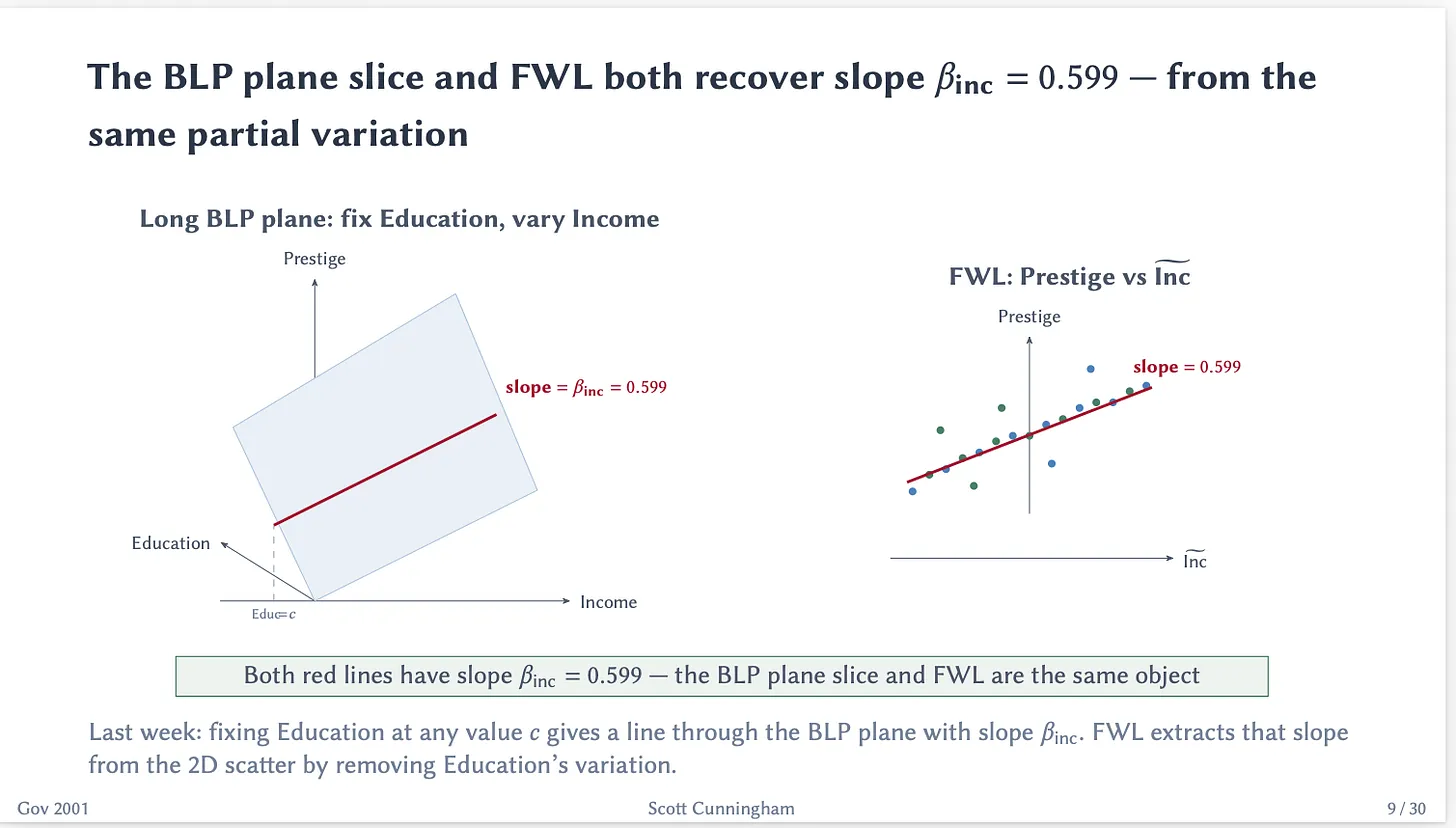
\includegraphics[width=0.85\textwidth,height=0.78\textheight,keepaspectratio]{fwl.png}
\end{center}

\end{frame}

\begin{frame}[fragile]{\texttt{/beautiful\_deck}}

\texttt{/beautiful\_deck} is built around a simple idea: a deck is not a document dump. It is rhetoric under time pressure.

\vspace{0.25cm}

\begin{verbatim}
https://github.com/scunning1975/mixtapetools

# Give Claude the repo link and say:
Read the MixtapeTools repo.
Install or adapt the beautiful_deck skill for this project.
Use the rhetoric-of-decks essay as the standard.
\end{verbatim}

\vspace{0.2cm}

\alert{This is production, but the standard is rhetorical: pathos, ethos, logos, low density, high impact.}

\end{frame}

\begin{frame}{Decks are rhetoric, not document dumps}

\texttt{/beautiful\_deck} sits on top of a short essay --- \emph{The Rhetoric of Decks}.

\vspace{0.25cm}

The standard is not coverage. It is persuasion under time pressure:

\begin{itemize}\setlength\itemsep{0.3em}
    \item titles are assertions, not labels
    \item one idea per slide
    \item ethos, pathos, logos --- in that order, every time
    \item beauty is function: every element earns its place
    \item compile clean. zero warnings. always.
\end{itemize}

\vspace{0.3cm}

\alert{The skill is not building slides. It is teaching the agent what a good talk looks like.}

\end{frame}

\begin{frame}{\texttt{/beautiful\_deck} compiles clean. \texttt{/tikz} sees what it cannot.}

\texttt{/beautiful\_deck} loops on overfull boxes, font warnings, undefined references --- the things \texttt{pdflatex} catches. It will not stop until they are gone.

\vspace{0.25cm}

\textbf{But \texttt{pdflatex} never warns} that a label sits on a Bezier curve, a legend overlaps the plot, or an axis title is clipped at the figure edge. \texttt{ggsave} does not refuse to write the PNG. The producing agent declares the figure done.

\vspace{0.2cm}

\textbf{LLMs have poor spatial reasoning over rendered output.} Eyeballing is unreliable. So \texttt{/tikz} replaces it with two mechanisms:

\begin{itemize}\setlength\itemsep{0.1em}
    \item \textbf{Math mode}: Bezier-curve geometry on the source --- chord length, bend angle, label safe zone
    \item \textbf{Visual mode}: multimodal vision on the rendered PNG, looking for the same three errors
\end{itemize}

\vspace{0.2cm}

\alert{Compile-clean is necessary. Visually clean is what makes the figure beautiful.}

\end{frame}

\begin{frame}{Example: clean a chaotic project folder}

Many research projects are not clean pipelines. They are sediment.

\vspace{0.25cm}

\begin{itemize}\setlength\itemsep{0.3em}
    \item old scripts with unclear order
    \item duplicated data and output files
    \item tables whose source is no longer obvious
    \item folders organized by memory, not documentation
    \item projects that become emotionally costly to reopen
\end{itemize}

\vspace{0.35cm}

\alert{A safe first agent task: inventory, map, and propose. Do not move or rewrite yet.}

\end{frame}

  \begin{frame}{Example: my Downloads folder}

  This is not a research project. It is where research materials, teaching files, installers, images, and forgotten data extracts accumulated.

  \vspace{0.18cm}

  \begin{center}
  \small
  \begin{tabular}{@{}lr@{}}
  \toprule
  Total files & \textbf{32,402} \\
  Top-level items & 336 \\
  Total size & \textbf{104 GB} \\
  Date range & May 2010 $\rightarrow$ today \\
  Top-level folders & 94 \\
  \bottomrule
  \end{tabular}
  \end{center}

  \vspace{0.1cm}

  {\small Top-level mix: 48 PNGs, 39 PDFs, 37 HEICs, 33 \texttt{.md}, 13 MP4s, 13 CSVs, 12 \texttt{.txt}, 11 MP3s, 7 forgotten \texttt{.dmg} installers, 6 \texttt{.docx}. The
  \texttt{.do}/\texttt{.tex}/\texttt{.dta} files didn't leave---they sank into subfolders (1{,}193 \texttt{.tex}, 1{,}428 CSVs, 1{,}041 \texttt{.dta} tree-wide).}

  \vspace{0.2cm}

  \alert{336 top-level items is already too many for Finder. So the first job is not cleanup. It is diagnosis.}

  \end{frame}

  \begin{frame}{The mess has a shape}

  The single largest item is a 24 GB folder named \texttt{154561-V1} --- not the IPUMS extract I assumed, but a forgotten openICPSR replication package stuffed with patent data.

  \vspace{0.3cm}

  \begin{itemize}\setlength\itemsep{0.3em}
      \item 19 GB in the \texttt{2026-03} folder --- mostly a 9.5 GB \texttt{cps\_00025.dat}, \emph{that} being the IPUMS CPS extract
      \item 9.3 GB of teaching folders
      \item eight ``Episode'' MP4s at 2.2--3.8 GB each
      \item the five biggest items account for about 64 GB of 104 GB
  \end{itemize}

  \vspace{0.35cm}

  \alert{This is exactly the kind of task where an agent can make the invisible structure visible before anyone touches a file.}

  \end{frame}

\begin{frame}{Two folder workflows}

\begin{columns}[T]
\begin{column}{0.48\textwidth}
\textbf{Clean an old project}

\vspace{0.15cm}
{\footnotesize
\texttt{Read this folder. Do not modify files.}\\
\texttt{Map data, code, outputs, and pipeline order.}\\
\texttt{Flag inconsistencies.}
}
\end{column}

\begin{column}{0.48\textwidth}
\textbf{Start correctly}

\vspace{0.15cm}
{\footnotesize
\texttt{github.com/scunning1975/mixtapetools}\\[0.15cm]
\texttt{/newproject my-project}
}

\vspace{0.1cm}
{\footnotesize Creates a standard scaffold: \texttt{CLAUDE.md}, \texttt{README.md}, \texttt{code/}, \texttt{data/}, \texttt{output/}, \texttt{documents/}, \texttt{decks/}, \texttt{notes/}, and \texttt{progress\_logs/}.}
\end{column}
\end{columns}

\vspace{0.25cm}

\alert{The shared principle: make structure visible before asking for judgment.}

\end{frame}


% =============================================================================
% TAMU NEW (2026-10-02): Hooks subsection (after Skills, before Verification)
% =============================================================================

% ---- divider ----
\begin{frame}[plain]
\vfill
\begin{center}
{\LARGE\bfseries\textcolor{charcoal}{Hooks: the rule the agent cannot skip}}\\[0.35cm]
{\large\textcolor{warmgray}{When prose is not enough, you reach for code}}
\end{center}
\vfill
\end{frame}

\begin{frame}{When prose fails, you reach for a hook}
Recall: \texttt{CLAUDE.md}, skills, prompts --- all prose, all \emph{cheap talk}. The model can skip any of them under load.
\vspace{0.3cm}
\begin{itemize}\setlength\itemsep{0.3em}
    \item \textbf{\texttt{CLAUDE.md}} --- what the agent \emph{knows}. A briefing.
    \item \textbf{Skills} --- what the agent \emph{can do}. A procedure you call by name.
    \item \textbf{Hooks} --- what the agent \emph{must do}. Code the harness runs, whatever the model decides.
\end{itemize}
\vspace{0.25cm}
\alert{How to know: reach for a hook only when a rule must hold \emph{every time} --- when ``please don't'' is not good enough.}
\end{frame}

\begin{frame}{What a hook is --- and who made it}
A \textbf{hook} is a shell command the harness runs \emph{automatically} at a fixed moment in the agent's lifecycle --- not when the model chooses, but every time.
\vspace{0.3cm}
\begin{itemize}\setlength\itemsep{0.28em}
    \item \textbf{Who.} Anthropic's Claude Code engineers shipped them in 2025 --- a feature of the tool, not something the model writes for itself.
    \item \textbf{The moments.} \texttt{PreToolUse} (before a tool runs), \texttt{PostToolUse} (after), plus session start/stop, prompt-submit, pre-compact.
    \item \textbf{Why.} The model is probabilistic; a hook is deterministic. It fires whether the agent cooperates or not.
\end{itemize}
\vspace{0.15cm}
\alert{A skill is advice the agent may take. A hook is a gate it cannot walk around.}
\end{frame}

\begin{frame}[fragile]{How a hook works --- and the simplest one}
You register it in \texttt{.claude/settings.json}: a \emph{matcher} (which tool) and a \emph{command}. The event arrives as JSON on \texttt{stdin}; \textbf{exit 0 allows, exit 2 blocks} and hands your message back to the agent.
\vspace{0.15cm}
\begin{verbatim}
"PostToolUse": [{ "matcher": "Edit|Write",
  "hooks": [{ "type": "command",
              "command": "black $CLAUDE_PROJECT_DIR" }]}]
\end{verbatim}
\vspace{0.05cm}
That is a whole hook: after every edit, run the formatter. No script needed.
\vspace{0.15cm}
\alert{Any language --- a bash one-liner, Python, Node. Mine live in \texttt{hooks/*.py}, registered in \texttt{settings.json}.}
\end{frame}

\begin{frame}{What makes a great hook}
\begin{itemize}\setlength\itemsep{0.28em}
    \item \textbf{Structural, not textual.} Match a named field --- the file \emph{path} --- not words in the agent's text. A constructed path defeats any string-matcher by construction.
    \item \textbf{Narrow.} Near-zero false positives. A hook that cries wolf trains you to ignore it.
    \item \textbf{Fail-open on errors.} A malformed event must never wedge the session --- but fail \emph{closed} on the thing it guards.
    \item \textbf{Speak plainly.} Hand back one clear sentence, not a cryptic \texttt{errno}.
    \item \textbf{A tripwire, not the whole wall.} The hook is the fast top layer; the real guarantee lives deeper.
\end{itemize}
\end{frame}

\begin{frame}{My five hooks at a glance}
\begin{center}
\footnotesize
\renewcommand{\arraystretch}{1.25}
\begin{tabular}{@{}llp{5.5cm}@{}}
\toprule
\textbf{Hook} & \textbf{Fires on} & \textbf{Enforces} \\
\midrule
\texttt{protect-raw-data} & Pre: Edit/Write & raw data is immutable --- never overwrite \texttt{data/raw/} \\
\texttt{no-fabricated-exhibit} & Pre: Edit/Bash & no figure from made-up data (unless a labeled Monte Carlo) \\
\texttt{no-offbook-exhibit} & Pre: Bash & no figure drawn inline in a shell --- only named scripts \\
\texttt{deck-from-pipeline} & Post: Edit/Write & no decked exhibit unless a wired script rebuilds it \\
\texttt{no-stale-canon} & Post: Edit/Write & warn if a ``canon'' exhibit is missing, unwired, or stale \\
\bottomrule
\end{tabular}
\end{center}
\vspace{0.25cm}
\alert{Every one guards the same chain: real data $\rightarrow$ named code $\rightarrow$ exhibit $\rightarrow$ deck.}
\end{frame}

\begin{frame}{\texttt{protect-raw-data}: the data is immutable}
\textbf{Fires} before any \texttt{Edit}/\texttt{Write} whose target is an \emph{existing} file in \texttt{data/raw/}. Blocks it --- but adding a \emph{new} raw file is fine.
\vspace{0.3cm}
\begin{itemize}\setlength\itemsep{0.25em}
    \item \textbf{The rule:} raw source data is never modified. Every transform \emph{reads} raw and \emph{writes} to \texttt{data/derived/}.
    \item \textbf{Structural:} it resolves the real path (symlinks, \texttt{..}, case) --- not a word-scan.
    \item It hands back a sentence, not an \texttt{errno}: ``read it; write transformed output to \texttt{derived/}.''
\end{itemize}
\vspace{0.15cm}
\alert{This is the fast top layer. The real wall is a root-owned vault --- which is where we'll push on it, live, at the end.}
\end{frame}

\begin{frame}{\texttt{no-fabricated-exhibit}: never a made-up number}
\textbf{Fires} when a figure/table script contains synthetic-data language \emph{and} a random-number generator --- on \texttt{Write}, and on the \texttt{Bash} that runs it.
\vspace{0.3cm}
\begin{itemize}\setlength\itemsep{0.25em}
    \item \textbf{The incident (2026-07-17):} a teaching slide drew \emph{illustrative} synthetic data with a footnote. It slipped past every other guard because it came through a figure script.
    \item \textbf{Carve-out:} a labeled Monte Carlo (a \texttt{\# MONTE CARLO} header) passes.
    \item A footnote is not a defense. The number must trace to real data.
\end{itemize}
\vspace{0.1cm}
\alert{My first rule, turned into a gate: never present a figure that doesn't trace to real, unmodified data.}
\end{frame}

\begin{frame}{The pipeline pair: every exhibit must be reproducible}
\textbf{\texttt{no-offbook-exhibit}} (before a Bash run). Blocks drawing a figure \emph{inline} in a shell --- \texttt{python -c "...savefig..."}, a heredoc. A picture with no producer file can't be re-run or audited. Every exhibit is born in a named script.
\vspace{0.35cm}
\textbf{\texttt{deck-from-pipeline}} (after an edit to a deck). Blocks a deck that references a figure \emph{no script wired into} \texttt{run\_pipeline.sh} produces. ``Ran once in chat'' is not enough.
\vspace{0.2cm}
\alert{The incident: a whole outcome built ad-hoc in chat, decked anyway --- caught only by memory. Now the machine catches it.}
\end{frame}

\begin{frame}{\texttt{no-stale-canon}: the certainty fence}
\textbf{Fires} when I mark a stage's exhibits ``canon'' --- done. It checks each one and \emph{warns} (does not block) if it is:
\vspace{0.25cm}
\begin{itemize}\setlength\itemsep{0.22em}
    \item \textbf{missing} --- the file isn't on disk
    \item \textbf{unwired} --- no pipeline script rebuilds it
    \item \textbf{stale} --- the figure is \emph{older} than the script that makes it
\end{itemize}
\vspace{0.2cm}
Why it exists, in my words: \emph{``if I'm going to make 5$\times$ as much stuff, I need to be 5$\times$ as sure it's right.''}
\vspace{0.1cm}
\alert{Hanging a figure that was never remade is exactly the silent failure my memory can't catch. The hook can.}
\end{frame}

\begin{frame}{``The problem with hooks is you have to debug them''}
An engineer at Netflix told me that --- half-joking. His point: skills feel easy, so we love them. Hooks are \emph{code}.
\vspace{0.3cm}

And he's right. A hook runs silently, outside the conversation. When it misfires it blocks the wrong thing, or fails with a cryptic error --- and you debug it like any program.
\vspace{0.25cm}
\begin{itemize}\setlength\itemsep{0.22em}
    \item \texttt{protect-raw-data} took a three-agent red team --- and two whole arms I built and then \emph{deleted}.
    \item every hook here is a few rounds of false positives I had to sand off.
\end{itemize}
\vspace{0.05cm}
\alert{Skills are prose you write once. Hooks are software you maintain.}
\end{frame}

\begin{frame}{But the debugging is the price of a guarantee}
Here is what the joke hides: a hook can enforce \emph{precisely because} it is code. Skills feel easy because they're cheap talk --- and cheap talk is what fails under load.
\vspace{0.3cm}
\begin{itemize}\setlength\itemsep{0.28em}
    \item a hook fails \textbf{loud} --- a block, right now. A skill fails \textbf{quiet} --- a plausible wrong number you find months later.
    \item debugging the hook is how I learned where the \emph{real} wall is: the raw-data hook taught me the guarantee lives in the kernel, not the script.
\end{itemize}
\vspace{0.12cm}
\alert{Pay the debugging tax for the few rules that must hold. Leave everything else to prose.}
\end{frame}

\begin{frame}{Live: let's try to break the raw-data hook}
Now we debug one together --- by attacking it. I point aggressive agents at \texttt{protect-raw-data} and tell them to overwrite a raw file any way they can.
\vspace{0.3cm}
\begin{itemize}\setlength\itemsep{0.25em}
    \item constructed paths, symlinked parents, case tricks, a heredoc that writes then runs
    \item we watch which get blocked --- and which expose a gap
\end{itemize}
\vspace{0.25cm}
When I did this before, a three-agent red team \emph{broke the clever version}. The fix wasn't a cleverer hook --- it was a \emph{smaller} one, plus a root-owned vault.
\vspace{0.1cm}
\alert{A textual guard loses to a constructed path by construction. The kernel is the guard that can't be hacked.}
\end{frame}

% =============================================================================
\section{Verification}
% =============================================================================

\begin{frame}{Verification is the new bottleneck}

Agents make production cheap enough to separate from verification.

\vspace{0.4cm}

\begin{center}
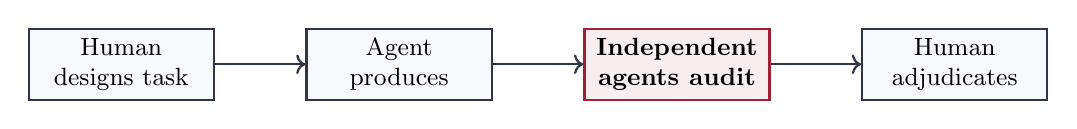
\begin{tikzpicture}[
    node distance=1.15cm,
    box/.style={rectangle, draw=charcoal, thick, fill=lightbg,
                minimum width=2.35cm, minimum height=0.85cm, align=center, font=\small},
    audit/.style={rectangle, draw=mitcardinal, thick, fill=mitcardinal!8,
                minimum width=2.35cm, minimum height=0.85cm, align=center, font=\small\bfseries}
]
    \node[box] (human) {Human\\designs task};
    \node[box, right=of human] (produce) {Agent\\produces};
    \node[audit, right=of produce] (audit) {Independent\\agents audit};
    \node[box, right=of audit] (judge) {Human\\adjudicates};

    \draw[->,thick,charcoal] (human) -- (produce);
    \draw[->,thick,charcoal] (produce) -- (audit);
    \draw[->,thick,charcoal] (audit) -- (judge);
\end{tikzpicture}
\end{center}

\vspace{0.45cm}

\textbf{The bottleneck moves.} The hard part is no longer producing first drafts, first regressions, or first summaries.

\vspace{0.25cm}

\alert{The hard part is designing verification systems that survive cheap production.}

\end{frame}

\begin{frame}{Verification systems have design ingredients}

Do not ask whether one output ``looks right.'' Ask how the workflow makes errors visible.

\vspace{0.25cm}

Useful ingredients:

\begin{itemize}\setlength\itemsep{0.3em}
    \item independent starts
    \item narrow assignments
    \item adversarial roles
    \item cross-language checks
    \item forced comparison against source material
\end{itemize}

\vspace{0.1cm}
\alert{The unit of trust is the workflow, not the single answer.}

\end{frame}

\begin{frame}{Audits are one way to buy verification}

Four empirical-research audits I use as verification tools:

\vspace{0.25cm}

\begin{enumerate}\setlength\itemsep{0.45em}
    \item \textbf{Literature audit} --- one agent per cited paper, checking accuracy against source text.
    \item \textbf{Rhetoric audit} --- one agent turns a paper into a talk; another judges whether the story is faithful.
    \item \textbf{Behavior audit} --- many agents become experimental units, revealing how agents behave under constraints.
    \item \textbf{Implementation audit} --- independent agents re-run the same analysis across languages or packages.
\end{enumerate}

\vspace{0.35cm}

\begin{center}
\alert{The goal is not audit for its own sake. The goal is confidence that the claim, code, citation, or estimate is right.}
\end{center}

\end{frame}


\begin{frame}[shrink=8]{Borrow templates; use what you actually understand}

\small
\textbf{Two public starter templates}, both worth a look:

\begin{itemize}\setlength\itemsep{0.08em}
    \item \textbf{Clo-Author} (Hugo Sant'Anna) --- per-paper pipeline: lit discovery, paper review, methods checks, writing, submission. {\scriptsize \texttt{hsantanna.org/clo-author/}}
    \item \textbf{Claude Code workflow} (Pedro Sant'Anna) --- per-researcher OS: slides, papers, replication, quality gates. {\scriptsize \texttt{psantanna.com/claude-code-my-workflow/}}
\end{itemize}

\vspace{0.2cm}

\textbf{What I actually do day to day:}
\begin{enumerate}\setlength\itemsep{0.08em}
    \item Drop the paper into \textbf{Refine.ink}, download the markdown report, walk through revisions with Claude. Pricey, but a desk reject is more expensive.
    \item Use my own \texttt{/referee2} constantly. Not because it's better --- because I built it, I understand it, and it conforms to my objectives.
\end{enumerate}

\vspace{0.15cm}

\alert{Borrow the template; build the routine. The thing you actually use needs to be the thing you understand.}

\end{frame}

\begin{frame}{MixtapeTools: \texttt{/referee2}}

\texttt{/referee2} is my verification routine for work I do not want the original producing agent to grade.

\vspace{0.3cm}

The core idea is independence:

\begin{itemize}\setlength\itemsep{0.35em}
    \item a fresh agent reads the artifact cold
    \item it checks code, tables, claims, or slides against source material
    \item for code, it can reimplement in another language
    \item for decks, it can audit rhetoric, density, compilation, and fidelity
\end{itemize}

\vspace{0.35cm}

\alert{The original agent can explain itself. A fresh verifier is more likely to catch what the first one normalized.}

\end{frame}


  \begin{frame}{OLS is deterministic, so three languages must agree}

  \texttt{/referee2} rebuilds the pipeline in Stata, R, and Python --- then compares the numbers.

  \vspace{0.3cm}

  The logic is that OLS is not a random process. It minimizes the sum of squared residuals, $\hat\beta = (X'X)^{-1}X'y$ --- a fixed function of the data.

  \vspace{0.3cm}

  \begin{itemize}\setlength\itemsep{0.35em}
      \item So coefficients, standard errors, $t$-stats, and the $F$ are the \emph{same real numbers} regardless of language.
      \item Agreement to six decimals across all three $\Rightarrow$ the pipeline is right.
      \item Disagreement is never noise. It is a bug, or a named package default (df adjustment, robust-SE flavor, missing-value handling) --- and the audit says which.
  \end{itemize}

  \vspace{0.35cm}

  \alert{LLM coding errors are orthogonal across languages. Three independent implementations converge only when none of them erred.}

  \end{frame}

\begin{frame}[fragile]{Save the work before the context dies}

Long agent sessions fail. The antidote is to make the project remember what happened.

\vspace{0.25cm}

\begin{verbatim}
Write a progress log in progress_logs/.
Summarize everything we have done since the last update:
- decisions made
- files read
- files changed
- remaining questions
- next safe steps
\end{verbatim}

\vspace{0.25cm}

Then a fresh agent can re-enter the folder, read the markdown logs, and continue without relying on the vanished chat.

\vspace{0.25cm}

\alert{Progress logs turn fragile conversations into durable project memory.}

\end{frame}

  \begin{frame}{I don't picture my work --- I remember it with my hands}

  I have \emph{aphantasia}: no mental images. When I recall the past --- even my own memories --- the screen is black. I get the story and the feeling, never the picture.
  
  \vspace{0.25cm}
  
  So for twenty years I never \emph{saw} my projects. I knew them procedurally:
  
  \begin{itemize}\setlength\itemsep{0.3em}
      \item repetition --- opening the same files every morning
      \item the focus zone I'd drop into, picking up from yesterday
      \item a map of the project imprinted by hand, over years
  \end{itemize}

  \vspace{0.25cm}
  
  \alert{The projects I worked longest, I knew best. Memory was muscle, not image.}
  
  \end{frame}
  

  \begin{frame}{At arm's length, the muscle memory never forms}
  
  Agents moved me out of production. I'm faster --- and I never touch the files.
  
  \vspace{0.25cm}
  
  So the instincts I took for granted are simply gone. The basic questions come back:
  
  \begin{itemize}\setlength\itemsep{0.3em}
      \item which file made this figure?
      \item are these outputs current, or stale?
      \item where am I in the project?
  \end{itemize}

  \vspace{0.25cm}
  
  \alert{It's like piloting a submarine by sonar after a career steering the ship by eye.}
  
  \end{frame}
  

  \begin{frame}{A day's context window has to be wiped --- on purpose}
  
  After a full day, the window is enormous. The model starts to drift: it forgets, repeats itself, spawns stray files, loses the thread.
  
  \vspace{0.25cm}
  
  So \texttt{/clear} isn't optional --- it's hygiene. But clearing erases the day.
  
  \vspace{0.35cm}
  
  \alert{If I have to wipe the conversation, the memory has to live \emph{outside} it --- on disk.}
  
  \end{frame}
  

  \begin{frame}{\texttt{/sleep}: write it all down before the window dies}
  
  The night tool. Its audience isn't me --- it's \emph{tomorrow's} me, who will remember nothing.
  
  \vspace{0.25cm}
  
  \begin{itemize}\setlength\itemsep{0.3em}
      \item a dated log in \texttt{audits/} --- decisions, changes, corrections, open threads
      \item \texttt{STATE.md}, the project's working memory --- objective, in progress, what's next
      \item a \emph{state-of-mind} note --- energy, what's settled, what still carries weight
  \end{itemize}

  \vspace{0.3cm}
  
  \alert{\texttt{/sleep} writes exactly what \texttt{/amnesia} will read.}
  
  \end{frame}


  \begin{frame}{\texttt{/amnesia}: rebuild the map every morning}
  
  The morning tool. It reads last night's \texttt{STATE.md} and newest log, then reorients me:
  
  \begin{itemize}\setlength\itemsep{0.3em}
      \item a short summary --- objective / just done / in progress / next
      \item a flip-through deck at \texttt{reorient/} for the visual reload
      \item then it walks me back in, question by question, until I'm oriented
  \end{itemize}

  \vspace{0.2cm}
  
  Always built from the current files --- never stale, regenerated every time.
  
  \vspace{0.3cm}
  
  \alert{\texttt{/amnesia} answers ``where am I?'' --- and because \texttt{/sleep} ran last night, the answer is true.}
  
  \end{frame}
  
  


% ============================ MEMORY-ARC CAPSTONE (loop diagram) ============================
\begin{frame}{The loop: the conversation dies, the memory doesn't}
\begin{center}
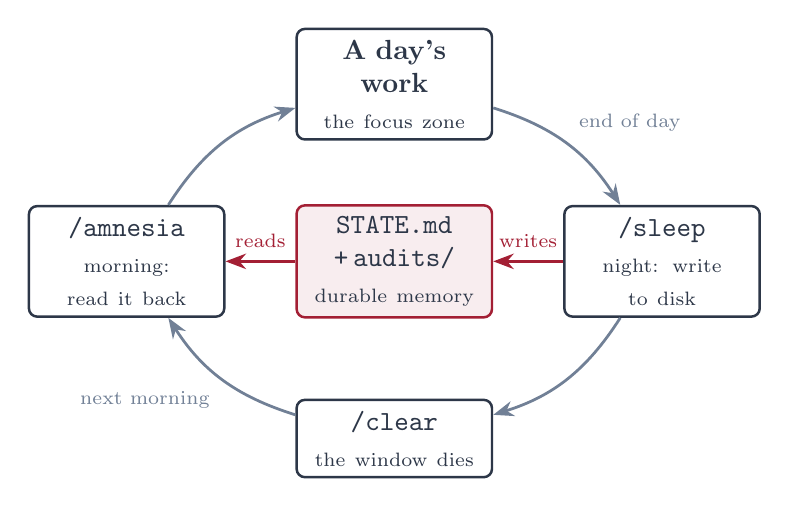
\begin{tikzpicture}[
  >={Stealth[length=2.6mm]},
  stage/.style={draw, rounded corners=3pt, line width=0.9pt, align=center,
                text width=2.2cm, minimum height=0.9cm, inner sep=4pt, fill=white, text=charcoal},
  cyc/.style={->, line width=1pt, warmgray},
  io/.style={->, line width=1.1pt, mitcardinal}
]
\node[stage, draw=charcoal] (work)    at (0,2.25)  {\textbf{A day's work}\\[1pt]\scriptsize the focus zone};
\node[stage, draw=charcoal] (sleep)   at (3.4,0)   {\texttt{/sleep}\\[1pt]\scriptsize night: write to disk};
\node[stage, draw=charcoal] (clear)   at (0,-2.25) {\texttt{/clear}\\[1pt]\scriptsize the window dies};
\node[stage, draw=charcoal] (amnesia) at (-3.4,0)  {\texttt{/amnesia}\\[1pt]\scriptsize morning: read it back};
\node[stage, draw=mitcardinal, fill=mitcardinal!8] (disk) at (0,0)
     {\texttt{STATE.md}\\\texttt{+\,audits/}\\[1pt]\scriptsize durable memory};
\draw[cyc] (work)    to[bend left=20] node[above right=1pt, font=\scriptsize, text=warmgray]{end of day} (sleep);
\draw[cyc] (sleep)   to[bend left=20] (clear);
\draw[cyc] (clear)   to[bend left=20] node[below left=1pt, font=\scriptsize, text=warmgray]{next morning} (amnesia);
\draw[cyc] (amnesia) to[bend left=20] (work);
\draw[io] (sleep) -- node[above=1pt, font=\scriptsize, text=mitcardinal]{writes} (disk);
\draw[io] (disk)  -- node[above=1pt, font=\scriptsize, text=mitcardinal]{reads}  (amnesia);
\end{tikzpicture}
\end{center}
\alert{\texttt{/clear} wipes the window every day. The disk is what survives it.}
\end{frame}

% =============================================================================
% TAMU NEW: Mixtape Harness section
% =============================================================================
\section{Mixtape Harness}

\begin{frame}{Memory keeps me oriented. A harness keeps me honest.}
The \texttt{/sleep}--\texttt{/amnesia} loop solves one failure: \emph{where am I?}
\vspace{0.3cm}

It does not solve the other. With an agent producing faster than I can check, I \emph{skip steps} --- and never feel the skip.
\vspace{0.35cm}

\alert{So I built a harness: a checklist for causal inference, turned into machinery, that will not let me run ahead of my own verification.}
\end{frame}

\begin{frame}{Experts skip steps --- and AI makes the skip silent}
\textbf{Gawande, \emph{The Checklist Manifesto}.} It is not novices who skip steps under load. It is \emph{experts}. Overconfidence scales \emph{with} skill --- which is why pilots and surgeons still use written checklists.
\vspace{0.3cm}

\textbf{What AI changed.} Producing and verifying used to be one motion --- I understood the code because I wrote it. Now:
\begin{itemize}\setlength\itemsep{0.22em}
    \item the agent writes 200 lines in one shot
    \item I can approve work I did not produce and do not fully understand
    \item the agent is confident even when wrong --- so the skip is silent
\end{itemize}
\vspace{0.2cm}

\alert{The harness re-couples production and verification --- it restores what working through agents took away.}
\end{frame}

\begin{frame}{Rubin: design trumps analysis}
\textbf{Rubin (2008), \emph{For Objective Causal Inference, Design Trumps Analysis}.}
\vspace{0.3cm}

Objectivity is not rescued at the analysis stage with a clever regression. It is \emph{built at the design stage, before you ever see the outcome.}
\vspace{0.3cm}
\begin{itemize}\setlength\itemsep{0.22em}
    \item a randomized experiment is trusted because it is outcome-blind --- you \emph{cannot} tune it to the answer
    \item an observational study earns that trust only by imposing the same blindness: reconstruct the experiment, find the assignment mechanism, balance covariates --- outcomes hidden
\end{itemize}
\vspace{0.2cm}

\alert{``Final outcome data cannot be used in design without compromising the objectivity of the study design.''}
\end{frame}

\begin{frame}{The design happens before you look at the outcome}
Rubin's discipline, in order:
\begin{enumerate}\setlength\itemsep{0.2em}
    \item \textbf{Name} the hypothetical experiment the data pretend to be.
    \item \textbf{Find} the assignment mechanism --- who was treated, and why?
    \item \textbf{Hide} the outcomes; design on covariates only.
    \item \textbf{Balance} --- and where there is no overlap, \emph{refuse} to infer.
    \item \textbf{Only then} analyze. The smallest, last step.
\end{enumerate}
\vspace{0.25cm}

\alert{The harness keeps the outcome ``not available at this stage'' --- on purpose, the way randomization does it for free.}
\end{frame}

\begin{frame}{The same discipline, written as checklists}
\textbf{Imbens.} His surveys --- including Imbens \& Xu's (2024) reassessment of LaLonde --- make the case in the selection-on-observables world: check overlap, check balance, run sensitivity, \emph{systematically}. Design first.
\vspace{0.3cm}

\textbf{The Mixtape.} Every chapter ends the same way: a checklist, or practical do-this-then-that tips --- one per research design.
\vspace{0.3cm}

\alert{The harness is that tradition condensed into something an agent and I walk together, top to bottom.}
\end{frame}

\begin{frame}{The harness: Rubin's line, turned into machinery}
\texttt{github.com/scunning1975/mixtape\_harness} --- clone it, point it at a study, it enforces the discipline.
\vspace{0.25cm}
\begin{columns}[T]
\begin{column}{0.5\textwidth}
\begin{itemize}\setlength\itemsep{0.18em}
    \item \textbf{The law} --- \texttt{CLAUDE.md}: zero-error as a \emph{constraint}
    \item \textbf{The checklists} --- the design steps, gated
    \item \textbf{The stages} --- one room per step, re-enterable
\end{itemize}
\end{column}
\begin{column}{0.5\textwidth}
\begin{itemize}\setlength\itemsep{0.18em}
    \item \textbf{The dashboard} --- live, reads disk, colors drift
    \item \textbf{The instruments} --- \texttt{/pipeline}, \texttt{/referee2}, \texttt{/covariates}
    \item \textbf{Working memory} --- \texttt{STATE.md}
\end{itemize}
\end{column}
\end{columns}
\vspace{0.25cm}

\alert{The estimator will not run until the design steps before it are signed off. That gate is the whole point.}
\end{frame}

\begin{frame}{The pipeline is the ground truth}
Every table and figure in the paper is produced by \emph{pipelined code} --- scripts that, at the end, re-run from raw data to rebuild the entire analysis.
\vspace{0.3cm}
\begin{itemize}\setlength\itemsep{0.22em}
    \item nothing in the paper is hand-made or remembered --- it is \emph{regenerated}
    \item every figure traces back to the exact script that made it
    \item \texttt{/pipeline} re-derives all of it, so ``is this output stale?'' has an answer
\end{itemize}
\vspace{0.25cm}

\alert{If it is not produced by the pipeline, it is not evidence. Provenance is the antidote to amnesia.}
\end{frame}

\begin{frame}{The diff is the unit of observation --- but I am not Paul}
In the IDE, with code review (a PR, or \texttt{gh}), I watch the \emph{diffs} --- every change the agent makes.
\vspace{0.25cm}

\textbf{Paul Goldsmith-Pinkham:} ``the diff is the unit of observation.'' Review every one.
\vspace{0.25cm}

\textbf{Honestly, for me that is not quite true.} Paul has the memory and the spatial instinct to hold the whole diff-space. I don't --- so I do what I \emph{can}: I follow one thread, aggressively. And my first thread is always the same.
\vspace{0.15cm}

\alert{Bite. Before anything downstream: did the treatment actually \emph{do something}?}
\end{frame}

\begin{frame}{Checklist: target, then bite}
\textbf{1 $\cdot$ Target estimand.} Write it in potential outcomes --- ATT? group-time? --- for a named population, with a weighting rule. Decide it \emph{first}; every later step serves this one parameter.
\vspace{0.4cm}

\textbf{2 $\cdot$ Bite.} Show the treatment's first stage: did it move the thing that is supposed to move the outcome? Maps, time series, the assignment mechanism --- \emph{shown before the outcome.}
\vspace{0.3cm}

\alert{Bite sits on the design side of Rubin's line. Outcome last.}
\end{frame}

\begin{frame}{Checklist: covariates \& balance, then sample shares}
\textbf{3 $\cdot$ Covariates \& balance.} Choose the $X$ that drive trends in the untreated outcome $Y(0)$ (Heckman-Ichimura-Todd). Check overlap; a normalized difference $>0.25$ is imbalanced (Imbens \& Rubin).
\vspace{0.4cm}

\textbf{4 $\cdot$ Sample shares.} Count treated units by cohort. Callaway-Sant'Anna weights by these shares --- so one big cohort can quietly dominate the aggregate.
\vspace{0.3cm}

\alert{Every N here must reconcile with the bite map --- no orphan units.}
\end{frame}

\begin{frame}{Checklist: outcome trends, then power}
\textbf{5 $\cdot$ Outcome trends.} Plot mean $Y$ by group --- \emph{pre-treatment only}. Do the groups move in parallel before treatment? \emph{Do not peek at post-outcomes yet} (Rubin).
\vspace{0.4cm}

\textbf{6 $\cdot$ Power / MDE.} What is the minimum detectable effect, given clusters, periods, and serial correlation (Bertrand-Duflo-Mullainathan)? Say what a null would --- and would not --- mean.
\vspace{0.3cm}

\alert{Power is recorded \emph{before} the estimator runs, so a null is interpretable later.}
\end{frame}

\begin{frame}{Checklist: estimator \& event study, then falsification}
\textbf{7 $\cdot$ Estimator \& event study.} Lock the sample (\texttt{/referee2 drift}), then run --- Callaway-Sant'Anna preferred. Plot the event study with a universal baseline.
\vspace{0.4cm}

\textbf{8 $\cdot$ Falsification \& sensitivity.} Placebo group, placebo outcome, pre-trends --- then Rambachan-Roth: how large a trend violation would it take to overturn the result?
\vspace{0.3cm}

\alert{The estimator is \emph{gated}: it will not run until steps 1--6 are signed off.}
\end{frame}

\begin{frame}{My first thread, always: does the law bite?}
\textbf{Rhode Island, with Manisha Shah.} In 2003 a court ruling accidentally decriminalized \emph{indoor} sex work. Before any downstream outcome I asked one question: \emph{did that event actually disrupt the market?}
\vspace{0.3cm}
\begin{itemize}\setlength\itemsep{0.18em}
    \item 15--20 qualitative interviews --- police chief, head of vice, ED doctors, the FBI, the state-police statistician, newspaper owners, the health department
    \item newspaper data, arrest data
    \item diff-in-diff and synthetic control --- did 2003 ``bite''?
\end{itemize}
\vspace{0.2cm}

\alert{Bite first: can I find \emph{any} evidence the law did what it was supposed to --- before chasing the downstream effects economists love?}
\end{frame}

\begin{frame}{Same move, now with Brazil: Dias \& Fontes (2024)}
Before homicides, before deaths of despair --- \emph{did the reform bite?}
\vspace{0.25cm}

\textbf{Dias \& Fontes (2024),} \emph{AEJ: Economic Policy}. Brazil's 2002 psychiatric reform rolled out \textbf{CAPS} --- community mental-health centers --- municipality by municipality through 2016.
\begin{itemize}\setlength\itemsep{0.18em}
    \item 5{,}180 municipalities, staggered adoption --- a textbook staggered DiD
    \item care shifts from the \emph{institution} to the \emph{community}
    \item outcomes: deaths of despair, and --- the headline --- \emph{homicides}
\end{itemize}
\vspace{0.15cm}

\alert{It is also the running example inside the harness --- so the shape of the analysis is already laid out.}
\end{frame}

\begin{frame}{The bite is two-sided: care up, institutions down}
\begin{center}
\small
\begin{tabular}{@{}lrr@{}}
\toprule
5-year ATT (per 10k) & Effect & vs.\ baseline \\
\midrule
\multicolumn{3}{@{}l}{\textit{Community care goes UP}}\\
\quad Outpatient MH procedures & $+264.2$ & $+113\%$ \\
\quad MH professionals & $+0.83$ & $+46\%$ \\
\midrule
\multicolumn{3}{@{}l}{\textit{Institutional care goes DOWN}}\\
\quad Psychiatric admissions & $-0.95$ & $-7.5\%$ \\
\quad\ \ long-stay schizophrenia & $-0.82$ & \\
\bottomrule
\end{tabular}
\end{center}
\vspace{0.25cm}

\alert{The same policy pushes one margin up and another down. For homicides, the causal first stage is the \emph{admissions drop} --- lost incapacitation.}
\end{frame}

\begin{frame}{Only one outcome moves --- and Penrose explains it}
\begin{center}
\small
\begin{tabular}{@{}lrl@{}}
\toprule
5-year ATT (per 10k) & Effect & \\
\midrule
Homicides & $+0.149$ & $+7.7\%$\; \textbf{(headline)} \\
Suicide & $0.002$ & ns \\
Deaths of despair & $-0.022$ & ns \\
Alcohol-related & $-0.018$ & ns \\
\bottomrule
\end{tabular}
\end{center}
\vspace{0.2cm}

\textbf{Penrose's hypothesis.} Move the crime-prone severely ill out of incapacitating institutions into under-resourced community care, and violence rises --- and the admissions drop is concentrated exactly in long-stay schizophrenia.
\vspace{0.15cm}

\alert{Deaths of despair are a true zero; homicides are the one thing that moves.}
\end{frame}

\begin{frame}{Every stage ships as a pull request}
As we walk the checklist, each stage is a diff you can see --- the pipeline script, plus the figure or table it produces.
\vspace{0.25cm}
\begin{itemize}\setlength\itemsep{0.22em}
    \item the \textbf{unit} is one exhibit --- the bite figure, the balance table, the event study
    \item the \textbf{PR} is the review --- you read the script diff \emph{and} look at the rendered output
    \item the \textbf{gate} is the merge --- the next stage does not start until this one is approved
\end{itemize}
\vspace{0.2cm}

\alert{Figures are where errors hide in plain sight. The loop exists to catch the exhibit that renders cleanly but is wrong.}
\end{frame}

\begin{frame}{The loop in action: fixing the bite figure}
The first exhibit is the bite --- psychiatric admissions down, outpatient care up. Watch one round:
\vspace{0.25cm}
\begin{enumerate}\setlength\itemsep{0.22em}
    \item Claude writes the pipeline script, renders the figure, and runs \texttt{gh pr create}.
    \item I review the diff and comment on the exact lines: \emph{``drop $g-1$, label the axis per 10k, trim p-score $>0.995$.''}
    \item \texttt{/loop 10m} picks up the comments, edits the script, re-renders, and pushes.
    \item The diff updates, the figure is right, I merge --- and the gate to Step 3 opens.
\end{enumerate}
\vspace{0.2cm}

\alert{The figure compiled fine the first time. It was still wrong. That is exactly what the loop is for.}
\end{frame}

\begin{frame}{Let's build it together --- and watch how I work}
We open the dashboard and walk the checklist on the Brazil data, in order:
\vspace{0.2cm}
\begin{enumerate}\setlength\itemsep{0.18em}
    \item establish the \textbf{bite} --- admissions down, outpatient up
    \item design outcome-blind --- target, covariates, balance, trends
    \item \emph{then} the estimator, the event study, the falsifications
    \item each one ships as a \textbf{pull request} --- you see the diff, you approve the merge
\end{enumerate}
\vspace{0.25cm}

\alert{Bite first, outcome last --- Rubin's line, enforced by the harness, with you watching every step.}
\end{frame}

% =============================================================================
% TAMU NEW: end Mixtape Harness section  (Verification content continues below)
% =============================================================================
\begin{frame}{Could I replicate the PNAS labeling for \$11?}

I wanted to see if I could replicate Card, Boustan and Abramitzky (PNAS 2022) on 140 years of US Congressional speeches --- but using OpenAI zero-shot instead of their fine-tuned RoBERTa.

\vspace{0.25cm}

\textbf{What they did.} Trained RoBERTa on $\sim$7{,}500 speeches hand-labeled by roughly a dozen Princeton students. Probably tens of thousands of dollars and weeks-to-months of human time. \emph{Cost-prohibitive for most resource-constrained researchers.}

\vspace{0.25cm}

\textbf{What I did.} Wrapped each segment in a short prompt, zero-shotted through the OpenAI Batch API on \texttt{gpt-4o-mini}. The hard part is getting the JSON formatting right --- which Claude is very good at handling.

\vspace{0.25cm}

\textbf{Cost.} About \textbf{\$11} and one hour. Then I had Claude produce the comparison against their published labels.

\end{frame}

\begin{frame}{Independent labeling tracks Card--Boustan--Abramitzky across 140 years}

\begin{center}
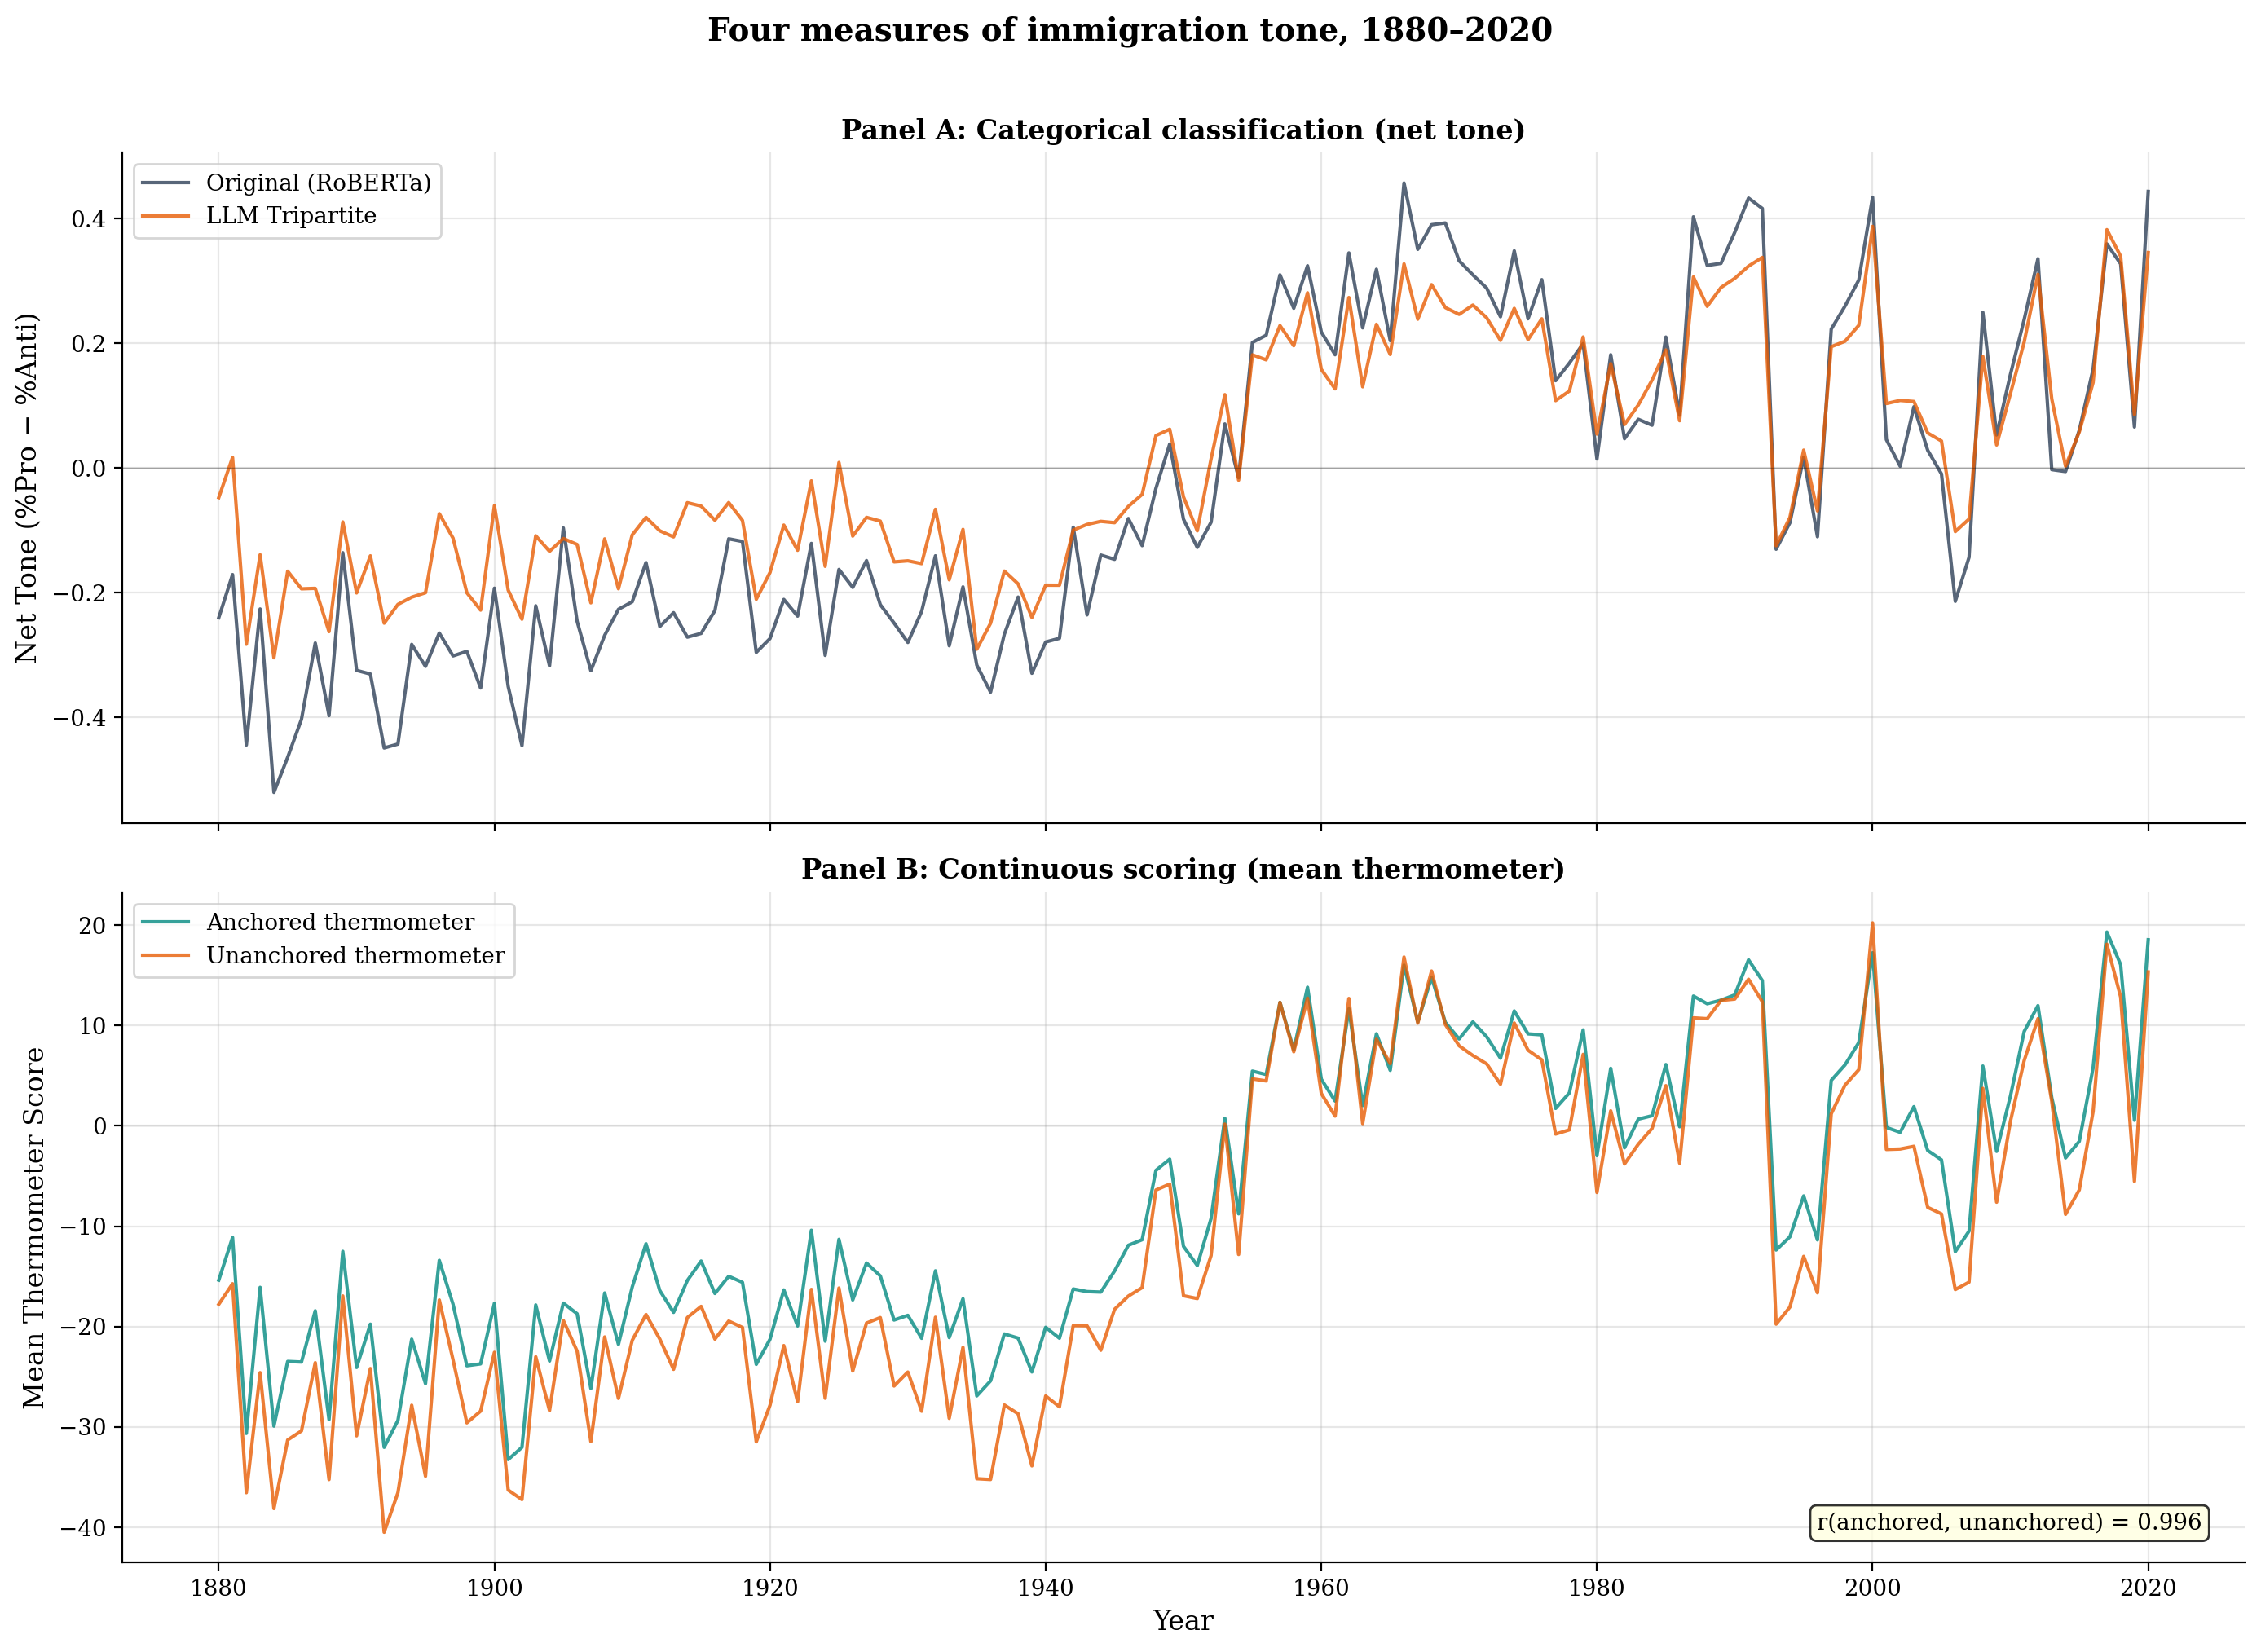
\includegraphics[width=0.66\textwidth,height=0.52\textheight,keepaspectratio]{unanchored_net_tone_comparison.png}
\end{center}

\textcolor{warmgray}{\scriptsize Net-tone trajectory: zero-shot \texttt{gpt-4o-mini} on 305{,}000 Congressional speech segments vs.\ Card-Boustan-Abramitzky's RoBERTa (PNAS 2022). No fine-tuning. No human annotators.}

\vspace{0.1cm}

\alert{This is what verification looks like when the production process is replaced.}

\end{frame}

\begin{frame}{Independent implementations turn disagreement into evidence}

Replicating analysis in a different language is not about new data. It is about verifying the original implementation.

\vspace{0.35cm}

\textbf{The logic:} syntax errors are probabilistic and language-specific.

\begin{itemize}\setlength\itemsep{0.25em}
    \item A merge error in R will not reproduce identically in Stata.
    \item A package-specific fallback in Python will not usually mimic one in R.
    \item Agreement rules out a wide class of bugs; disagreement tells you where to look.
\end{itemize}

\vspace{0.35cm}

\alert{This is the principle behind \texttt{/referee2}: a cold-start agent reimplements the analysis independently.}

\end{frame}

\begin{frame}{Verification works when errors are imperfectly correlated}

No checker is the oracle. The point is to compare independent error processes.

\vspace{0.3cm}

\begin{center}
\small
\begin{tabular}{@{}lll@{}}
\toprule
Checker 1 & Checker 2 & What disagreement reveals \\
\midrule
Agent & fresh agent & prompt- or context-specific errors \\
Agent & human RA & machine vs.\ human blind spots \\
R code & Stata/Python code & implementation-specific bugs \\
Manuscript & source paper & citation and interpretation errors \\
\bottomrule
\end{tabular}
\end{center}

\vspace{0.35cm}

\alert{The standard is zero avoidable errors. One pass is not enough.}

\end{frame}

\begin{frame}{Coefficient extraction at scale}

I gave many agents a corpus of $\sim$600 \textbf{APE} papers (Social Catalyst Lab's autonomously generated empirical-policy corpus) and asked them to extract every regression coefficient and standard error.

\vspace{0.3cm}

\begin{itemize}\setlength\itemsep{0.25em}
    \item agents read PDFs, located tables, emitted structured rows
    \item I built my own t-statistic distribution from the extracted data
    \item I planned to run Brodeur-style p-hacking diagnostics on top
\end{itemize}

\vspace{0.3cm}

\alert{Production was the means. The point of doing it was to verify a claim.}

\end{frame}

\begin{frame}{The first pass looked like p-hacking}

The Brodeur ratio came in around \textbf{1.52}. Excess mass piled up at $|t|=2$.

\vspace{0.3cm}

\begin{center}
\textit{Initial reading: AI-generated empirical papers carry the same publication-bias signature as the human literature.}
\end{center}

\vspace{0.45cm}

\alert{This was the wrong reading.}

\end{frame}

\begin{frame}{Non-random heaping I didn't see}

\begin{columns}[T]
\begin{column}{0.55\textwidth}
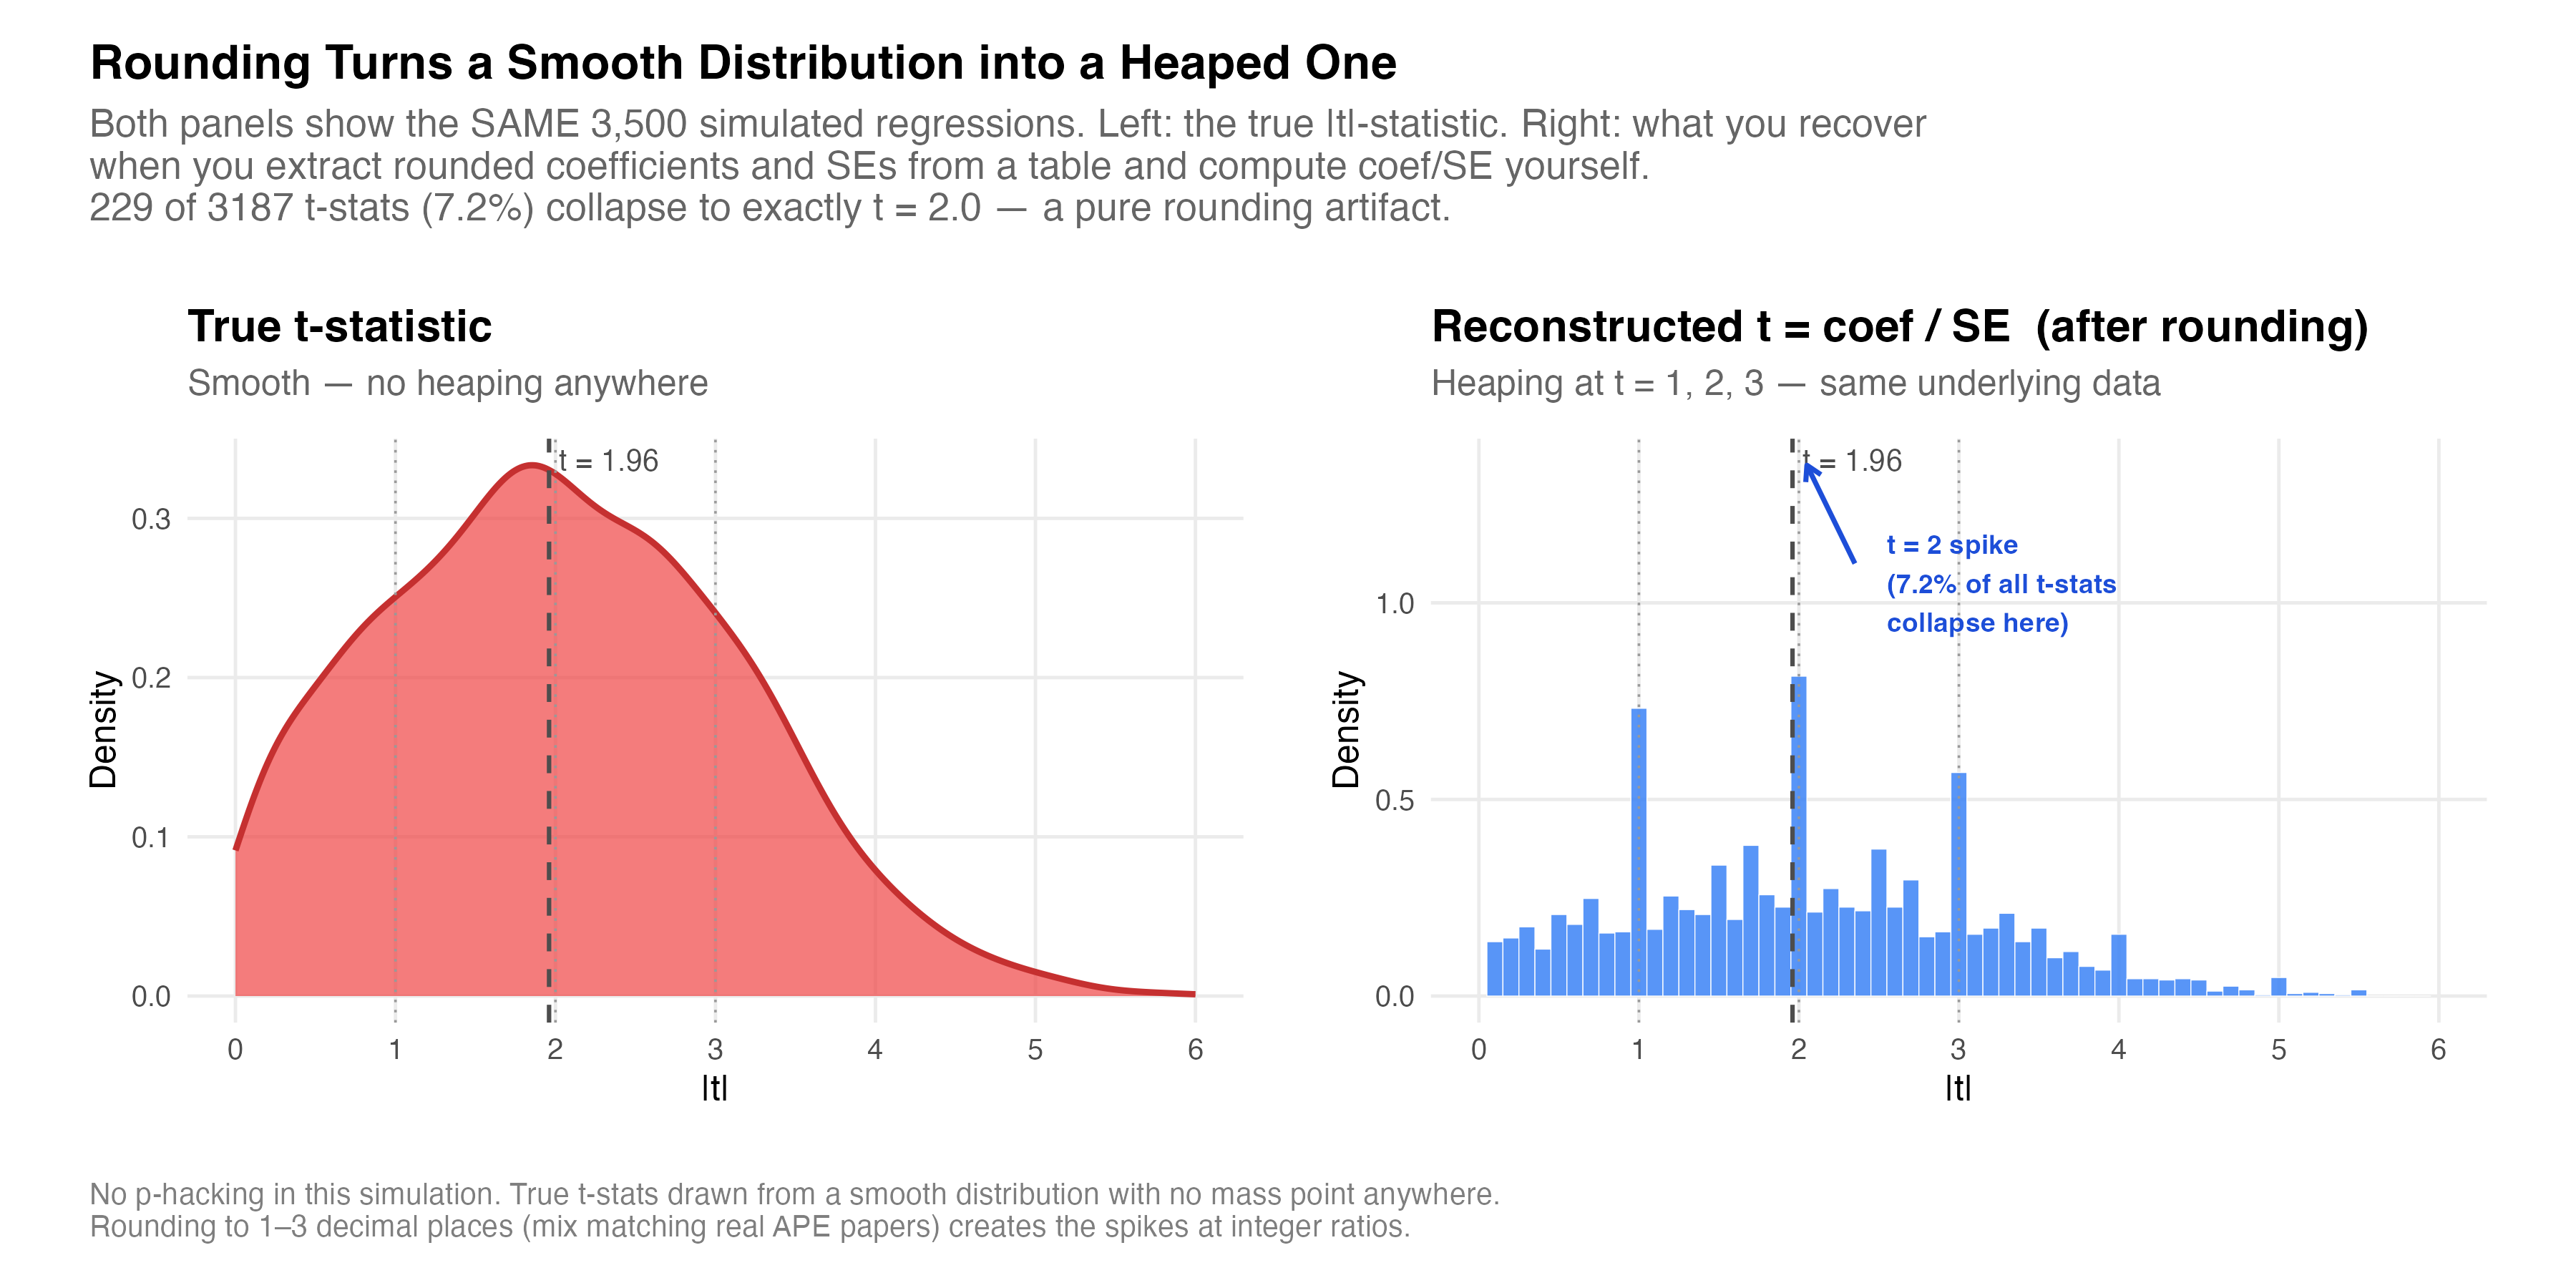
\includegraphics[width=\textwidth,keepaspectratio]{fig_sim_twopanel.png}
\end{column}

\begin{column}{0.42\textwidth}
\footnotesize
Coefficients and SEs in published papers are rounded. Dividing a rounded coefficient by a rounded SE piles $t$ up at integer ratios: 1, 2, 3.

\vspace{0.2cm}

I simulated 3{,}500 regressions \emph{with no p-hacking}. Same heaping.

\vspace{0.2cm}

Removing 68 exact-$t=2$ rows dropped the Brodeur ratio from 1.52 to \textbf{1.02}. Brodeur et al.\ have since acknowledged the issue.

\vspace{0.2cm}

\textit{Jason Fletcher and Gorkem Ozer caught it. I did not.}
\end{column}
\end{columns}

\vspace{0.1cm}

\alert{This is the experience that led me to write \texttt{/blindspot} --- I had started to wonder if I was going to miss the obvious.}

\end{frame}

\begin{frame}{Even zero discretion leaves implementation risk}

\textbf{Independent Hallucination Errors.} A second experiment.

\vspace{0.4cm}

\begin{itemize}
    \item Replicate Dias \& Fontes (2024, \emph{AEJ: Economic Policy}) on the same CAPS data.
    \item \textbf{96 zero-discretion agents.} Every decision prescribed in advance.
    \item Vary only what the principal might otherwise vary silently: the package and the covariate set.
\end{itemize}

\vspace{0.4cm}

\begin{center}
\alert{Six implementations of the same estimator. Sixteen specifications. Same data, same method, same controls. They should agree.}
\end{center}
\end{frame}

\begin{frame}{Six packages implement the same estimator differently}

\begin{center}
\small
\begin{tabular}{@{}lll@{}}
\toprule
Package & Language & Author \\
\midrule
\texttt{did} & R & Callaway \& Sant'Anna \\
\texttt{ddml} & R & Ahrens, Hansen, Schaffer, Wiemann \\
\texttt{csdid} & Stata & Rios-Avila \\
\texttt{csdid2} & Stata & Rios-Avila \\
\texttt{differences} & Python & Dionisi \\
\texttt{diff-diff} & Python & Gerber \\
\bottomrule
\end{tabular}
\end{center}

\vspace{0.5cm}

All using doubly robust + not-yet-treated controls + universal base period.

\vspace{0.35cm}

\alert{Identical specification across all six.}

\end{frame}

\begin{frame}{With no covariates, all six packages agree exactly}

\vspace{0.3cm}
\begin{center}
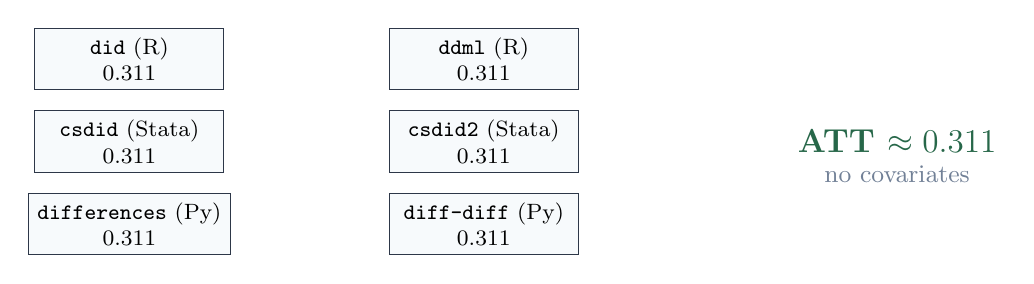
\begin{tikzpicture}[
  x=1.5cm, y=0.7cm,
  pkg/.style={rectangle, draw=charcoal, fill=lightbg, minimum width=2.4cm, minimum height=0.7cm, font=\footnotesize, align=center},
]
\node[pkg] at (0, 4) {\texttt{did} (R)\\$0.311$};
\node[pkg] at (3, 4) {\texttt{ddml} (R)\\$0.311$};
\node[pkg] at (0, 2.5) {\texttt{csdid} (Stata)\\$0.311$};
\node[pkg] at (3, 2.5) {\texttt{csdid2} (Stata)\\$0.311$};
\node[pkg] at (0, 1) {\texttt{differences} (Py)\\$0.311$};
\node[pkg] at (3, 1) {\texttt{diff-diff} (Py)\\$0.311$};
\node[font=\large\bfseries\color{forest}] at (6.5, 2.5) {ATT $\approx 0.311$};
\node[font=\small\color{warmgray}] at (6.5, 1.9) {no covariates};
\end{tikzpicture}
\end{center}

\vspace{0.4cm}

\begin{center}
\textit{The estimator itself is implemented correctly.}
\end{center}
\end{frame}

\begin{frame}{Add one covariate, and the agreement breaks}

\textbf{One covariate: \texttt{poptotaltrend} --- municipal population $\times$ year.}

\vspace{0.3cm}
\begin{center}
\small
\begin{tabular}{@{}lr@{}}
\toprule
Package & ATT \\
\midrule
\texttt{ddml} (R) & 0.45 \\
\texttt{csdid2} (Stata) & 0.45 \\
\texttt{did} (R) & 0.53 \\
\texttt{differences} (Python) & 0.67 \\
\texttt{csdid} (Stata) & \alert{1.15} \\
\texttt{diff-diff} (Python) & \alert{2.38} \\
\bottomrule
\end{tabular}
\end{center}

\vspace{0.4cm}

\begin{center}
\alert{Same data. Same estimator. Same single covariate. A 5$\times$ spread.}
\end{center}
\end{frame}

\begin{frame}{The disagreement fans out as covariates accumulate}
\begin{center}
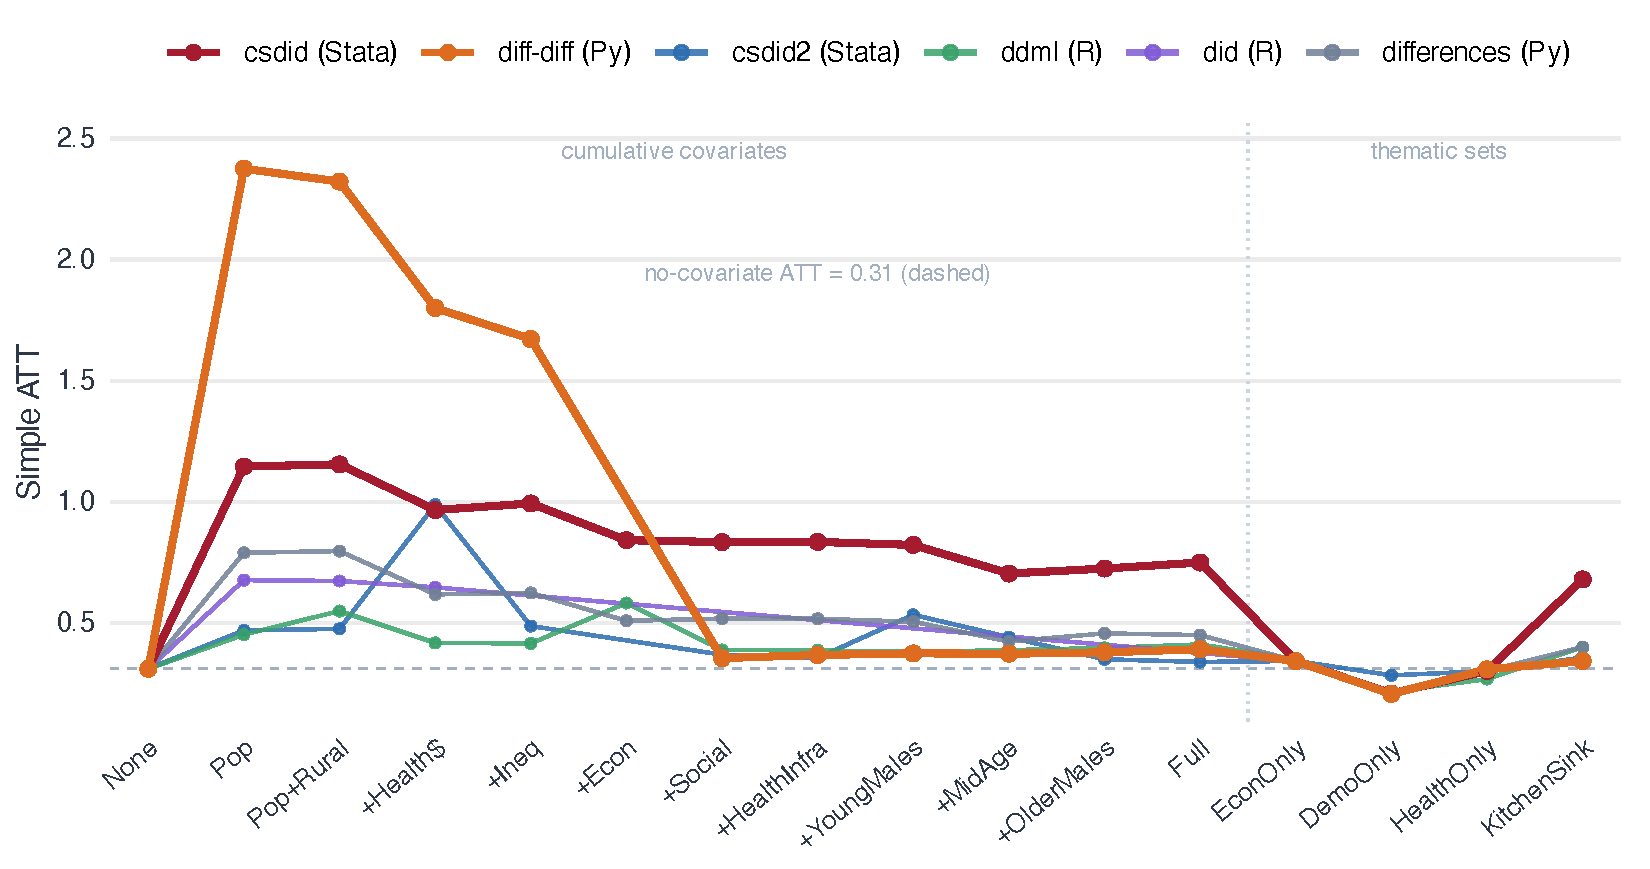
\includegraphics[width=0.84\textwidth,height=0.64\textheight,keepaspectratio]{specification_curve.pdf}
\end{center}

{\footnotesize\color{warmgray} Each line is one of six packages, plotted across 16 specifications. All start at the same point and then fan out.}
\end{frame}

\begin{frame}{The smoking gun: remove that one variable}

Run specs using only economics, demographics, or health covariates, excluding \texttt{poptotaltrend}.

\vspace{0.5cm}

\begin{center}
\textbf{All six packages agree to within 0.007.}
\end{center}

\vspace{0.5cm}

\alert{One variable caused the entire 5$\times$ spread.}

\end{frame}

\begin{frame}{The matrix inversion is the easy part}

The propensity-score logit's design matrix $X$ has a column \texttt{poptotaltrend} (population $\times$ year). For a 50{,}000-person municipality in 2010, that single cell is \textbf{100{,}500{,}000}. The variable lives on the order of $10^{10}$.

\vspace{0.25cm}

The other covariates live on the order of $0.01$ to $16{,}000$. Mixed in the same $X$, the condition number of $X'X$ explodes to roughly \textbf{$3.6\times 10^{9}$}.

\vspace{0.25cm}

Below machine epsilon ($2.22\times 10^{-16}$): the computer literally cannot distinguish the columns at 64-bit precision. Inverting $X'X$ --- which every propensity-score logit needs --- produces garbage.

\vspace{0.35cm}

\alert{But this is just a logistic regression. If $X'X$ is hard to invert, shouldn't \emph{all six} packages have a hard time with it?}

\vspace{0.15cm}

The answer turns out to be no.

\end{frame}

\begin{frame}{Six ``logistic regressions'' are not the same logistic regression}

\vspace{0.1cm}

\begin{center}
\scriptsize
\renewcommand{\arraystretch}{1.18}
\begin{tabular}{@{}llll@{}}
\toprule
Package & Lang & Routine called & Optimizer \\
\midrule
\texttt{did} & R & \texttt{glm(probit)} & IRLS \\
\texttt{ddml} & R & \texttt{glmnet} Lasso (DR) + \texttt{glm(probit)} trim & L1 coord.\ descent + IRLS \\
\texttt{csdid} & Stata & \texttt{probit, iterate(1000) difficult} + \texttt{drimp} & Newton--Raphson \\
\texttt{csdid2} & Stata & \texttt{probit, difficult ltol(0) tol(1e-5)} & Newton--R., relaxed tol. \\
\texttt{differences} & Py & \texttt{statsmodels.Probit().fit()} & statsmodels Newton \\
\texttt{diff-diff} & Py & \texttt{statsmodels.Probit()} + \texttt{CallawaySantAnna} & statsmodels + internal \\
\bottomrule
\end{tabular}
\end{center}

\vspace{0.3cm}

\alert{Same name on the API. Different optimizer. Different singular-matrix behavior. The user does not see this.}

\vspace{0.1cm}

{\scriptsize\color{warmgray} Each row is the actual call inside the package, recovered from the source.}

\end{frame}

\begin{frame}[shrink=8]{Is this wrong?}

\small
What we found:

\begin{itemize}\setlength\itemsep{0.1em}
    \item \texttt{did} \emph{silently} returns all-zero ATTs without raising
    \item \texttt{csdid} requires \texttt{iterate(1000) difficult} to nominally converge
    \item \texttt{csdid2} runs with relaxed tolerance: ``stabilized but not formally converged''
    \item \texttt{ddml}'s Lasso auto-standardizes inside the learner
    \item \texttt{statsmodels} converges silently --- possibly to wrong values
\end{itemize}

\vspace{0.2cm}

\textbf{Honest answer:} no individual choice is indefensible. Each package author made a reasonable engineering call. But the choice is invisible to the user. The documentation says ``logistic regression.''

\vspace{0.15cm}

\textbf{The new researcher degrees of freedom:} sort into language $\rightarrow$ package $\rightarrow$ hidden algorithmic action. Three layers; only the first appears in methods.

\vspace{0.15cm}

\textbf{The fix:} z-score the covariates, or divide \texttt{poptotaltrend} by $10^6$. The ill-conditioning is the trigger; remove the trigger and most of the divergence collapses.

\vspace{0.15cm}

\alert{Hidden actions become detectable only when independent agents replicate one another.}

\end{frame}

\begin{frame}[shrink=6]{Other issues found}

\small

\textbf{1.\ Cohort-specific propensity scores.} CS fits a separate propensity-score logit \emph{per treatment cohort}. With 500 treated municipalities split across cohorts, each PS regression sees only $N_c$ observations. If $k$ is too large for that $N_c$, you get erratic perfect separation --- wrapped inside the logistic, independent of the algorithmic heterogeneity above.

\vspace{0.3cm}

\textbf{2.\ Silent covariate dropping.} Some logistics, when they cannot estimate the full $X$, silently drop the covariates and regress $D$ on a constant only --- without telling the user. The package hides the propensity-score coefficient output and often does not store the propensity scores after estimation. The researcher --- and especially Claude in automation mode --- may not realize what just happened.

\vspace{0.3cm}

\alert{Hidden actions become detectable only when independent agents replicate one another.}

\vspace{0.1cm}

{\scriptsize\color{warmgray} Note: \texttt{diff-diff} (Gerber) has since been updated; the Round-4-era limitation has been addressed.}

\end{frame}

\begin{frame}{Agents make expensive verification routines cheap enough to run}

AI did not magically know the answer.

\vspace{0.35cm}

The workflow made the discrepancy visible:

\begin{itemize}\setlength\itemsep{0.3em}
    \item many independent agents
    \item multiple languages
    \item six packages
    \item forced comparison to a common target
\end{itemize}

\vspace{0.35cm}

\alert{Agents are useful because they make expensive verification routines cheap enough to run.}

\end{frame}

% =============================================================================
\section{What To Do Monday Afternoon}
% =============================================================================

\begin{frame}{Start with audits whose outputs you can judge}

Start with audits whose outputs you can inspect:

\vspace{0.2cm}

\begin{enumerate}\setlength\itemsep{0.25em}
    \item \textbf{Citation audit:} Does my literature review accurately represent each cited paper?
    \item \textbf{Repo audit:} Can a fresh agent install, run, and map this replication package?
    \item \textbf{Code audit:} Can a fresh agent reimplement my analysis in another language?
    \item \textbf{Referee audit:} What would a skeptical reader attack first?
    \item \textbf{Deck audit:} Does my presentation make one clear claim per slide?
\end{enumerate}

\vspace{0.25cm}

\alert{Do not begin with the task you least understand. Begin where you can judge the output.}

\end{frame}

\begin{frame}{A good assignment makes the output inspectable}

Five assignment rules:

\vspace{0.25cm}

\begin{enumerate}\setlength\itemsep{0.3em}
    \item Give it a folder with the relevant files.
    \item State the role: producer, auditor, adversary, replicator.
    \item Make the output concrete: table, memo, deck, diff, error list.
    \item Force source-grounding: quote line numbers, cite files, compare outputs.
    \item Use fresh agents for verification.
\end{enumerate}

\vspace{0.25cm}

\alert{The unit of progress is not a clever prompt. It is a repeatable workflow.}

\end{frame}

\begin{frame}[fragile,shrink=6]{Homework: build a skill, do not just borrow one}

If you make only one skill after this talk, make it a citation-audit skill. Pick a repeating task and turn it into a procedure your agent can run.

\vspace{0.25cm}

\textbf{Why build instead of borrow.} Ethan Mollick has noted that open source for skills is not the same as open source for code. A skill carries the author's prompts, assumptions, and failure modes. The audit surface is fuzzier than source. You inherit what you install.

\vspace{0.2cm}

\textbf{Why I show you mine anyway.} The point is the pattern, not the prompt. Fork, rewrite, replace --- the right thing to copy is the design move, not the trust.

\vspace{0.2cm}

\begin{verbatim}
Help me create a citation-audit skill for my papers.
It should: identify each cited claim;
spawn one agent per cited paper; compare my claim to source;
return accurate / overstated / missing / unclear.
Ask me questions and iterate before writing the final skill.
\end{verbatim}

\end{frame}

\begin{frame}[shrink=6]{Budget for the real tool, not the demo tier}

Agentic research work is not the same as asking a chatbot one question.

\vspace{0.35cm}

For long-running tasks, you want the strongest available model and enough usage headroom:

\begin{itemize}\setlength\itemsep{0.35em}
    \item Agents read many files, write code, run it, hit errors, inspect output, and try again.
    \item Smaller or capped models may look fine in demos but time out once you depend on the workflow.
    \item The relevant comparison is not free vs.\ paid. It is whether the agent can finish the job.
\end{itemize}

\vspace{0.35cm}

As of this talk: \textbf{Codex is roughly half the monthly price of Claude Max} --- about \$100 vs.\ \$200.

\vspace{0.25cm}

\alert{If agents become part of your research process, buy enough model to avoid making the workflow brittle.}

\end{frame}

\begin{frame}{When agents fail, ask where the workflow failed}

When an LLM underdelivers, there are two possible explanations:

\vspace{0.3cm}

\begin{columns}[T]
\begin{column}{0.47\textwidth}
\begin{block}{Model failure}
\footnotesize
The model genuinely lacks the capability, knowledge, or reasoning required.
\end{block}
\end{column}
\begin{column}{0.47\textwidth}
\begin{block}{Workflow failure}
\footnotesize
The user assigned the wrong task, gave the wrong context, allowed too much discretion, or failed to verify.
\end{block}
\end{column}
\end{columns}

\vspace{0.4cm}

\alert{In my experience, workflow failure is usually the first suspect.}

\end{frame}

\begin{frame}{Deskilling is also a verification risk}
\vspace{-0.45cm}
\begin{columns}
\begin{column}{0.52\textwidth}
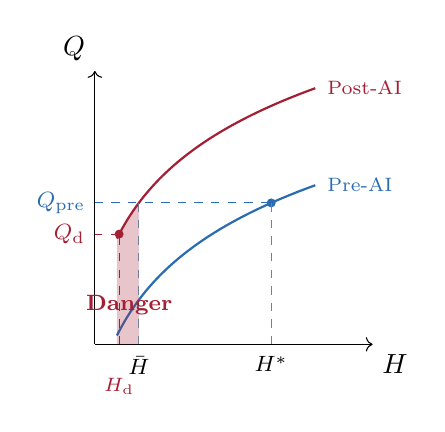
\begin{tikzpicture}[scale=0.56]
    \draw[->] (0,0) -- (6.3,0) node[below right] {$H$};
    \draw[->] (0,0) -- (0,6.2) node[above left] {$Q$};
    \draw[thick,ocean,domain=0.5:5,samples=100] plot (\x, {2.0*ln(\x+0.5)+0.2});
    \node[ocean,right,font=\scriptsize] at (5.05,3.610) {Pre-AI};
    \draw[thick,mitcardinal,domain=0.5:5,samples=100] plot (\x, {2.0*ln(\x+0.5)+2.4});
    \node[mitcardinal,right,font=\scriptsize] at (5.05,5.810) {Post-AI};
    \fill[mitcardinal,opacity=0.26]
        (0.5,0) -- plot[domain=0.5:1.0,samples=50] (\x, {2.0*ln(\x+0.5)+2.4})
        -- (1.0,0) -- cycle;
    \filldraw[ocean] (4,3.208) circle (2.5pt);
    \draw[dashed,ocean] (0,3.208) -- (4,3.208);
    \node[left,font=\footnotesize,ocean] at (0,3.208) {$Q_{\text{pre}}$};
    \node[below,font=\footnotesize] at (4,-0.05) {$H^*$};
    \draw[dashed,warmgray] (4,0) -- (4,3.208);
    \node[below,font=\footnotesize] at (1.0,-0.05) {$\bar{H}$};
    \draw[dashed,warmgray] (1.0,0) -- (1.0,3.208);
    \filldraw[mitcardinal] (0.55,2.50) circle (2.5pt);
    \draw[dashed,mitcardinal] (0.55,0) -- (0.55,2.50);
    \draw[dashed,mitcardinal] (0.55,2.50) -- (0,2.50);
    \node[below,font=\scriptsize,mitcardinal] at (0.55,-0.55) {$H_{\text{d}}$};
    \node[left,font=\footnotesize,mitcardinal] at (0,2.50) {$Q_{\text{d}}$};
    \node[mitcardinal,font=\footnotesize\bfseries] at (0.78,0.9) {Danger};
\end{tikzpicture}
\end{column}

\begin{column}{0.48\textwidth}
\small
AI can reduce the time and attention used in production.

\vspace{0.2cm}

That is the gain. But skill often came from exactly that time and attention.

\vspace{0.25cm}

\begin{itemize}\setlength\itemsep{0.18em}
    \item less production practice can mean less verification skill
    \item verification depends on accumulated judgment
    \item replication costs are falling toward zero
    \item outside scrutiny and penalties may rise
\end{itemize}

\vspace{0.25cm}

\alert{Be cognizant of the deskilling margin.}
\end{column}
\end{columns}
\end{frame}

\begin{frame}{The optimistic path is more verification per unit of attention}

Deskilling is possible. Lost attention is possible.

\vspace{0.35cm}

But the alternative is also possible:

\begin{itemize}\setlength\itemsep{0.35em}
    \item more citation claims checked against sources
    \item more replication packages actually run
    \item more code implemented twice
    \item more papers exposed to skeptical readers before submission
    \item more talks shaped around audience, not slide labor
\end{itemize}

\vspace{0.35cm}

\alert{The optimistic path is not less human judgment. It is more verification per unit of human attention.}

\end{frame}

\begin{frame}{The new skill is knowing what must be verified}

The scarce skill is not typing prompts.

\vspace{0.35cm}

The scarce skill is knowing:

\begin{itemize}\setlength\itemsep{0.35em}
    \item what to delegate
    \item what to constrain
    \item what to audit independently
    \item what disagreement means
    \item when the final judgment must be human
\end{itemize}

\vspace{0.45cm}

\begin{center}
\alert{AI agents make production cheap. The researcher's job is to make verification systematic.}
\end{center}

\end{frame}

\begin{frame}{Setup links are now an attack surface}

Agent workflows often ask you to copy commands into a terminal.

\vspace{0.25cm}

That changes phishing:

\vspace{0.15cm}

\begin{itemize}\setlength\itemsep{0.3em}
    \item cloned sites can imitate \texttt{claude.ai}, GitHub, or package docs
    \item a copy button can hide a dangerous install command
    \item agents can browse, compare domains, inspect repos, and explain commands
    \item do not paste terminal commands you do not understand
\end{itemize}

\vspace{0.25cm}

\alert{Use agents defensively too: ask them to verify the source before you trust the setup.}

\vspace{0.15cm}
{\scriptsize\color{warmgray} Recent threat reports: Google Threat Intelligence on AI-assisted social engineering; Cloud Security Alliance on indirect prompt injection.}

\end{frame}

% =============================================================================
% TAMU NEW (2026-10-01): Biases from Cues and Nudges
% Definitive, figure-backed minimum-wage agent experiment. Replaces old "three waves" prose.
% =============================================================================

% ---- transition divider ----
\begin{frame}[plain]
\vfill
\begin{center}
{\LARGE\bfseries\textcolor{charcoal}{Biases from Cues and Nudges}}\\[0.35cm]
{\large\textcolor{warmgray}{Can context quietly steer an agent toward a biased estimator?}}
\end{center}
\vfill
\end{frame}

% ---- concept ----
\begin{frame}{An experiment on the research process itself}
Cheap agents let me treat the agent as the experimental unit.
\vspace{0.3cm}
\begin{itemize}\setlength\itemsep{0.3em}
    \item Many agents receive the same data and the same task.
    \item I vary only the context around them, not the question.
    \item The outcome is behavioral: which econometrics does each agent choose?
\end{itemize}
\vspace{0.4cm}
\alert{The question is not whether an agent is right. It is whether the context moves what the agent does.}
\end{frame}

% ---- dataset ----
\begin{frame}{The data: U.S. state minimum wages, 1990 to 2022}
\begin{itemize}\setlength\itemsep{0.3em}
    \item A state-year panel of 51 states across 33 years.
    \item Outcome: the teen employment-to-population ratio.
    \item Treatment: a state's effective minimum wage binding above the federal floor.
    \item Variation: states raise their minimums on a staggered schedule, with federal increases layered on top.
\end{itemize}
\vspace{0.4cm}
\alert{Staggered timing is exactly the setting where the choice of estimator starts to matter.}
\end{frame}

% ---- TWFE bias: Goodman-Bacon ----
\begin{frame}{Under staggered timing, TWFE hides a bias term}
\vspace{0.2cm}
\begin{center}
{\large $\hat{\beta}^{\text{TWFE}} \;=\; \text{VWATT} \;+\; \text{VWPT} \;-\; \Delta\text{ATT}$}
\end{center}
\vspace{0.3cm}
\begin{itemize}\setlength\itemsep{0.3em}
    \item VWATT: a variance-weighted average of the true treatment effects.
    \item VWPT: a variance-weighted parallel-trends term.
    \item $\Delta$ATT: the penalty from using already-treated units as controls.
\end{itemize}
\vspace{0.35cm}
\alert{When effects grow or fade over time, the $\Delta$ATT term contaminates the estimate and can flip its sign.}
\vspace{0.1cm}
{\scriptsize\color{warmgray}Goodman-Bacon (2021).}
\end{frame}

% ---- why minimum wage (1) ----
\begin{frame}{Why the minimum wage, 1990 to 2022}
\begin{itemize}\setlength\itemsep{0.4em}
    \item \textbf{It is empirically contested.} The literature disagrees, so the training data carries no strong prior for the agent to lean on.
    \item \textbf{The federal floor rises during the panel.} Federal increases eventually bind everywhere, so there are no clean never-treated states left as controls.
\end{itemize}
\vspace{0.4cm}
\alert{A contested question with no clean controls is where estimator choice does the most damage.}
\end{frame}

% ---- why minimum wage (2): worst-case TWFE ----
\begin{frame}{A worst case for TWFE, and therefore a clean test}
\begin{itemize}\setlength\itemsep{0.3em}
    \item With a binary ``the minimum wage rose and binds'' indicator on the full panel, TWFE collapses to the sum of two 2$\times$2 comparisons: not-yet-treated and already-treated.
    \item The already-treated comparison is precisely the one that biases TWFE under staggering.
    \item Callaway--Sant'Anna can identify only binary ATTs between federal minimums; TWFE will accept any representation, binary or continuous dose.
\end{itemize}
\vspace{0.3cm}
\alert{So by construction, TWFE here is the biased estimator.}
\end{frame}

% ---- ground truth ----
\begin{frame}{The ground truth is not a number}
\begin{itemize}\setlength\itemsep{0.35em}
    \item I am not claiming the true employment effect of the minimum wage is some value.
    \item The ground truth is structural: in this design, TWFE is biased and Callaway--Sant'Anna is not.
\end{itemize}
\lead{So the clean behavioral question is whether a cue pushes an agent toward the estimator we already know is biased.}
\end{frame}

% ---- research question: hidden actions, cues, models ----
\begin{frame}{Do agents take hidden, unreported actions in response to cues?}
\vspace{0.1cm}
\begin{columns}[T]
\begin{column}{0.5\textwidth}
\textbf{Three cues}
\begin{itemize}\setlength\itemsep{0.3em}
    \item A JEL-style methodology document.
    \item An estimator menu.
    \item A preregistration plan.
\end{itemize}
\end{column}
\begin{column}{0.46\textwidth}
\textbf{Two models}
\begin{itemize}\setlength\itemsep{0.3em}
    \item GPT-5.5 (closed weight).
    \item Kimi K2.6 (open weight).
\end{itemize}
\end{column}
\end{columns}
\vspace{0.45cm}
\alert{A hidden action is the agent quietly switching estimators in response to context it was never told to obey.}
\end{frame}

% ---- the statistics ----
\begin{frame}{Simple statistics, read across the treatment arms}
\begin{itemize}\setlength\itemsep{0.35em}
    \item A linear probability model of choosing TWFE on the cue.
    \item A regression of the reported ATT estimate on the cue.
    \item A Kolmogorov--Smirnov test on the distribution of estimates across arms.
\end{itemize}
\vspace{0.3cm}
The same logic covers the other hidden actions: opening the preregistration plan, and redefining treatment as a continuous dose.
\vspace{0.3cm}
\alert{Nothing fancy. The design does the work, not the estimator.}
\end{frame}

% ---- figure A: three cues ----
\begin{frame}{Every cue moves the estimator}
\vspace{0.1cm}
\begin{center}
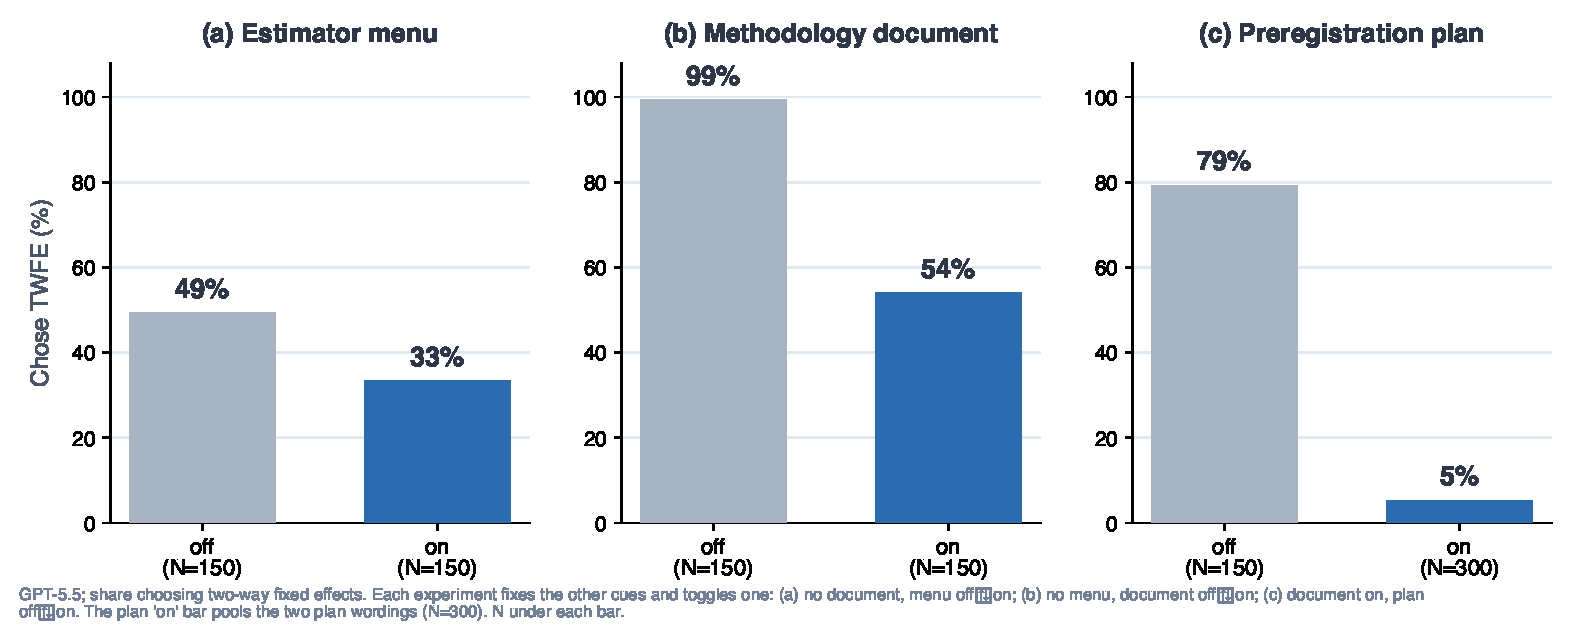
\includegraphics[width=\textwidth,height=0.66\textheight,keepaspectratio]{figA_three_cues}
\end{center}
\vspace{-0.05cm}
{\footnotesize\color{warmgray} GPT-5.5. Share choosing TWFE with each cue off vs on; the other cues are held fixed.}
\end{frame}

% ---- figure chain: prereg ----
\begin{frame}{A preregistration plan, read unprompted, reshapes the analysis}
\vspace{0.03cm}
\begin{center}
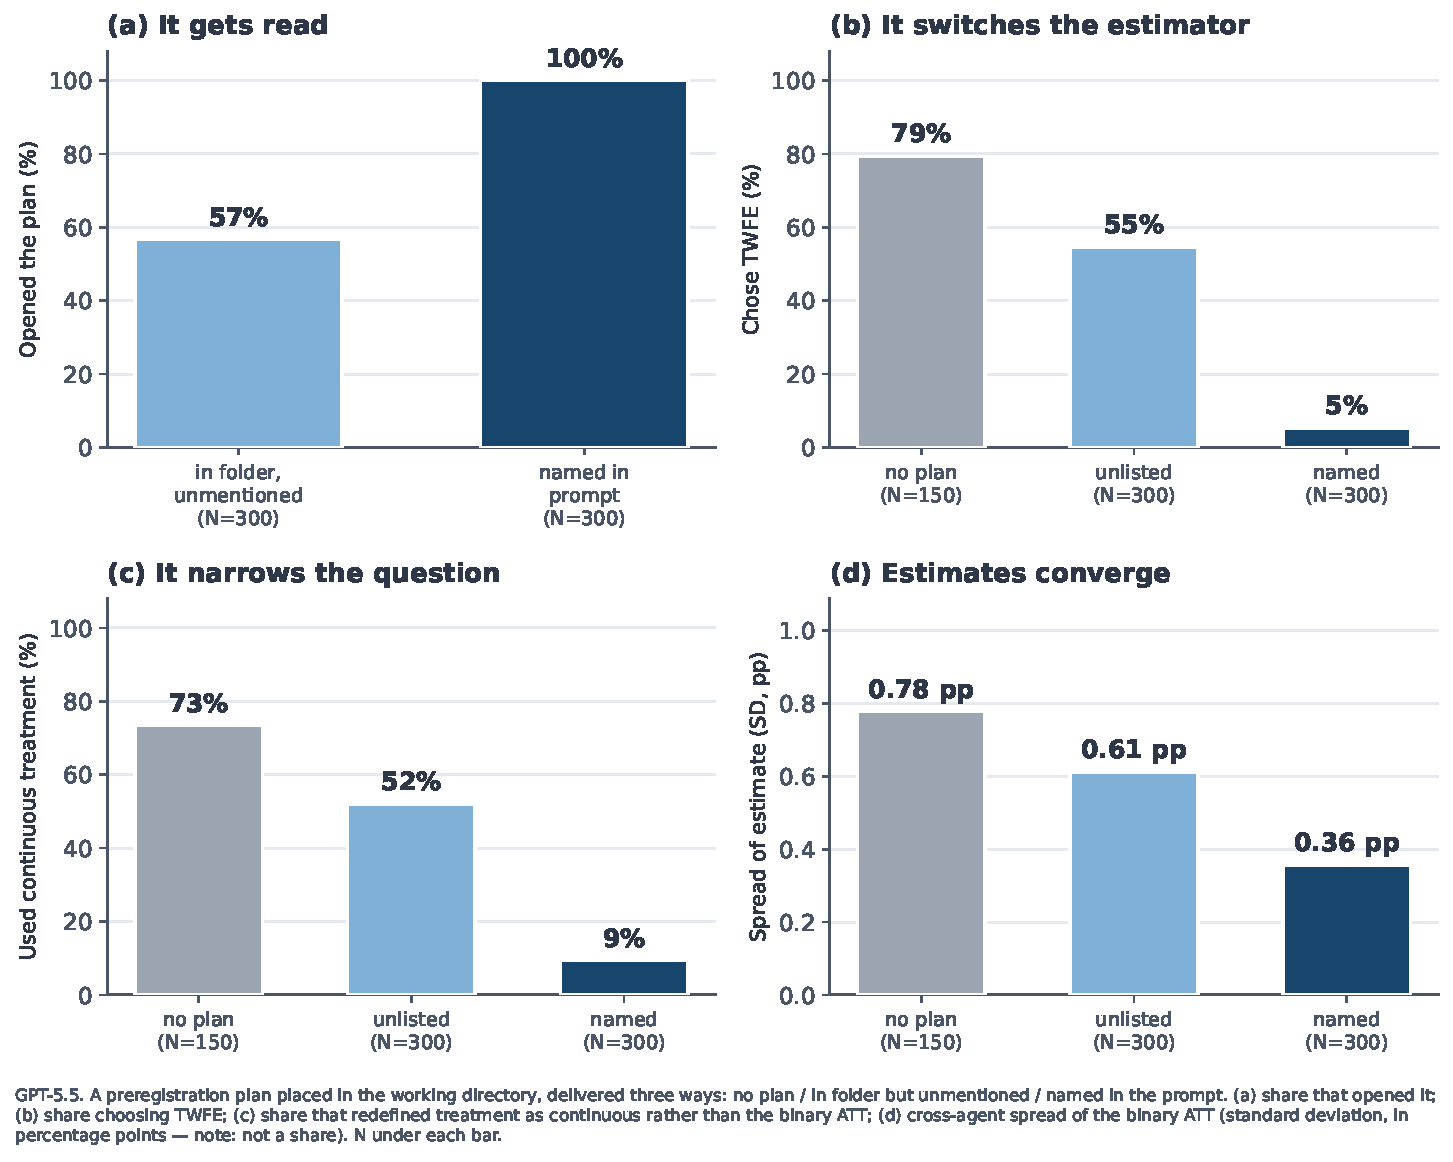
\includegraphics[width=\textwidth,height=0.76\textheight,keepaspectratio]{figChain_prereg}
\end{center}
\end{frame}

% ---- figure compare: gpt vs kimi ----
\begin{frame}{The same pull, in a closed model and an open one}
\vspace{0.1cm}
\begin{center}
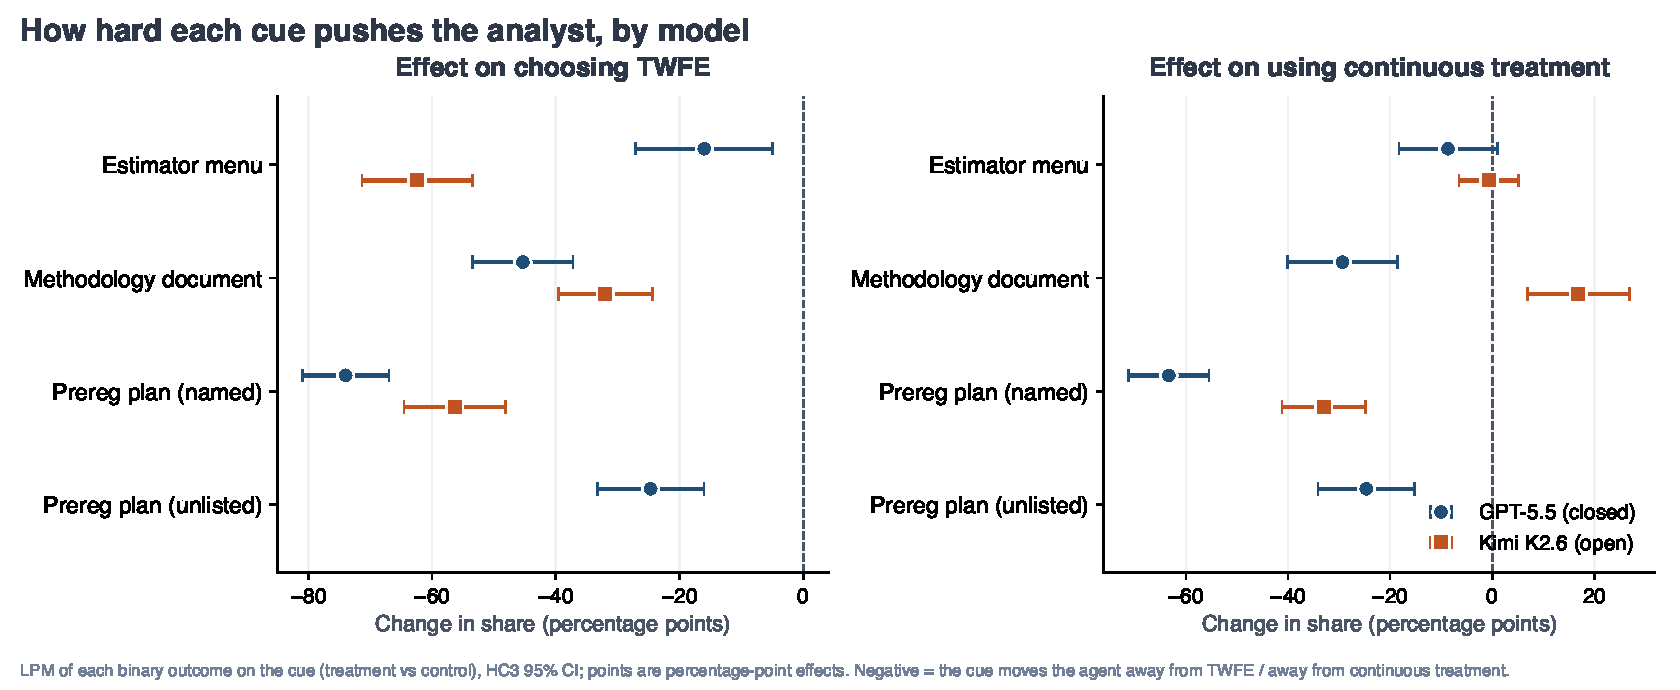
\includegraphics[width=\textwidth,height=0.65\textheight,keepaspectratio]{figCompare_coef}
\end{center}
\vspace{-0.05cm}
{\footnotesize\color{warmgray} Each point is an LPM of the outcome on the cue, HC3 95\% CI. Negative means the cue moves the agent away from TWFE.}
\end{frame}

% ---- lesson: hands on the wheel ----
\begin{frame}{Keep your hands on the wheel}
\begin{itemize}\setlength\itemsep{0.35em}
    \item The agents took these actions on their own, and did not report them.
    \item A cue you never considered can change the estimator, the estimand, and the estimate.
\end{itemize}
\lead{You cannot hand off the wheel. You have to understand the analysis, direct it, and verify it.}
\end{frame}

\begin{frame}{When agents fail, what failed?}

It is too simple to call every bad output a hallucination.

\vspace{0.3cm}

\begin{columns}[T]
\begin{column}{0.31\textwidth}
\begin{block}{Production failed}
\footnotesize
The agent made the wrong thing: bad code, bad draft, bad search, bad translation.
\end{block}
\end{column}
\begin{column}{0.31\textwidth}
\begin{block}{Verification failed}
\footnotesize
The output looked plausible, but nobody checked the right object.
\end{block}
\end{column}
\begin{column}{0.31\textwidth}
\begin{block}{Direction failed}
\footnotesize
The human gave the wrong task, context, constraints, or stopping rule.
\end{block}
\end{column}
\end{columns}

\vspace{0.4cm}

\begin{center}
\alert{My prior: workflow failures explain more agent failures than people think.}
\end{center}

\end{frame}


% =============================================================================
\section{Looking Ahead}
% =============================================================================
% TAMU NEW (2026-10-01): closing section. Sources: Acemoglu and Johnson (2024); Thompson (1963); Hobsbawm (1952).

\begin{frame}{It once sounded silly to call a machine a substitute for thinking}

For two hundred years, machines replaced muscle and then routine. Thinking was ours.

\vspace{0.35cm}

\begin{itemize}\setlength\itemsep{0.35em}
    \item In $Q = f(H, M)$, machine time now stands in for human time in cognitive work.
    \item That is the flat isoquant from this morning.
    \item I think that is where we are, and it is early.
\end{itemize}

\vspace{0.4cm}

\alert{I do not know where this is going. I do not think anyone does.}

\end{frame}

\begin{frame}{Are we complements or substitutes in the new production function?}

\begin{columns}[T]
\begin{column}{0.47\textwidth}
\textbf{If we are complements}
\begin{itemize}\setlength\itemsep{0.3em}
    \item The machine makes our time more productive.
    \item Demand for our time rises.
    \item This was true of the tools we grew up with.
\end{itemize}
\end{column}
\begin{column}{0.47\textwidth}
\textbf{If we are substitutes}
\begin{itemize}\setlength\itemsep{0.3em}
    \item The machine does the task in our place.
    \item Demand for our time falls.
    \item What remains for us is whatever the machine cannot do.
\end{itemize}
\end{column}
\end{columns}

\vspace{0.3cm}

The answer need not be the same for every task, or for every person.

\vspace{0.2cm}

And substitution is only half of it: if cheaper output raises demand enough, the output effect can outweigh the substitution effect.

\vspace{0.2cm}

\alert{It is an empirical question, and the data are not in.}

\end{frame}

\begin{frame}{Computers hollowed out the middle. Will agents hollow out the top?}

\textbf{What David Autor showed about computers}
\begin{itemize}\setlength\itemsep{0.3em}
    \item Computers took over routine tasks, which were the core of middle-skill jobs.
    \item Clerical and production work shrank as a share of employment.
    \item Jobs grew at the top and at the bottom, and the middle thinned.
\end{itemize}

\vspace{0.3cm}

\textbf{What we cannot yet say about agents}
\begin{itemize}\setlength\itemsep{0.3em}
    \item The tasks at risk now are analysis, writing, and code.
    \item Those belong to the upper middle class and the lower upper class.
\end{itemize}

\vspace{0.3cm}

\alert{Whether that tier hollows out the way the middle did is really unclear.}

\vspace{0.05cm}
{\scriptsize\color{warmgray}Autor, Levy, and Murnane (2003); Autor (2015).}

\end{frame}

\begin{frame}{The old tools are as useful as they ever were}

\begin{itemize}\setlength\itemsep{0.5em}
    \item \textbf{Production theory.} Isoquants, marginal products, and the elasticity of substitution tell us what to measure.
    \item \textbf{Labor markets tied to product markets.} The demand for our labor is derived from the demand for what we make.
    \item \textbf{The circular flow.} Someone's spending is someone else's income, including when the spender is a data center.
\end{itemize}

\vspace{0.45cm}

\alert{The world is more complicated than it was two years ago. The economics we already have is still how to think about it.}

\end{frame}

\begin{frame}{We have been here before: the first machines made the weavers rich}

\textbf{Cotton spinning was mechanized first.}

\vspace{0.0cm}

\begin{center}
\footnotesize
\begin{tabular}{@{}lr@{}}
\toprule
\textbf{Hours of labor to spin 100 pounds of cotton} & \\
\midrule
By hand, early 1700s & more than 50,000 \\
Crompton's mule, 1780 & 2,000 \\
Power-assisted mules, about 1795 & 300 \\
\bottomrule
\end{tabular}
\end{center}

\vspace{0.05cm}

\begin{itemize}\setlength\itemsep{0.25em}
    \item Yarn became cheap, and cheap yarn needed weavers.
    \item In its golden age, from about 1780 to 1800, a weaver worked four days a week and earned 40 shillings.
\end{itemize}

\vspace{0.1cm}

\alert{The first machine was a complement. That is why economists assumed machinery was painless.}

\vspace{0.05cm}
{\scriptsize\color{warmgray}Acemoglu and Johnson (2024), drawing on Chapman (1987).}

\end{frame}

\begin{frame}{Then the machines came for weaving}

\begin{columns}[c]
\begin{column}{0.42\textwidth}
\centering
{\footnotesize
\begin{tabular}{@{}lr@{}}
\toprule
\textbf{Year} & \textbf{Power looms in Britain} \\
\midrule
1813 & 2,400 \\
1820 & 14,150 \\
1833 & at least 100,000 \\
\bottomrule
\end{tabular}}
\end{column}
\begin{column}{0.54\textwidth}
\begin{itemize}\setlength\itemsep{0.3em}
    \item At first the power loom was hardly faster than a handloom.
    \item By the mid-1820s, one boy tending two looms could match fifteen cottage weavers.
    \item Spinning was already mechanized, so there was no neighboring trade to absorb them.
\end{itemize}
\end{column}
\end{columns}

\vspace{0.45cm}

\alert{The same industry, one generation later, and this time the machine was a substitute.}

\vspace{0.05cm}
{\scriptsize\color{warmgray}Acemoglu and Johnson (2024), drawing on Baines (1835) and Landes (2003).}

\end{frame}

\begin{frame}{The Luddites were skilled workers defending a trade}

\begin{itemize}\setlength\itemsep{0.4em}
    \item They began in Nottinghamshire in March 1811, among the framework knitters.
    \item In 1812 the movement spread to the cloth finishers of Yorkshire and the cotton weavers of Lancashire.
    \item They signed their letters ``Ned Ludd,'' a man who never existed.
    \item They broke particular machines: the ones being used to cut pay and to replace trained hands.
\end{itemize}

\vspace{0.4cm}

\alert{They were not afraid of technology. They were bargaining over who would bear its cost.}

\vspace{0.05cm}
{\scriptsize\color{warmgray}Thompson (1963); Hobsbawm (1952).}

\end{frame}

\begin{frame}{The government answered with soldiers and the gallows}

\begin{itemize}\setlength\itemsep{0.4em}
    \item In 1812 Parliament made breaking a machine punishable by death.
    \item About 12,000 soldiers were sent to the textile districts.
    \item In January 1813, seventeen men were hanged at York.
\end{itemize}

\vspace{0.35cm}

The workers had no vote, and unions were illegal.

\vspace{0.35cm}

\alert{Eric Hobsbawm called machine breaking ``collective bargaining by riot.'' It was the only bargaining they were allowed.}

\vspace{0.05cm}
{\scriptsize\color{warmgray}Thompson (1963); Hobsbawm (1952).}

\end{frame}

\begin{frame}{What they lost was autonomy, and not only income}

\begin{columns}[T]
\begin{column}{0.47\textwidth}
\textbf{At the handloom}
\begin{itemize}\setlength\itemsep{0.3em}
    \item The weaver chose when to work and how hard.
    \item The family worked together, at home.
    \item He sold cloth, and he did not sell his labor.
\end{itemize}
\end{column}
\begin{column}{0.47\textwidth}
\textbf{In the mill}
\begin{itemize}\setlength\itemsep{0.3em}
    \item The owner set the hours and the pace.
    \item The work was watched and it was monotonous.
    \item Owners hired women and children, who were cheaper and easier to control.
\end{itemize}
\end{column}
\end{columns}

\vspace{0.4cm}

E.\ P.\ Thompson's phrase for the change: a self-motivated man became a ``hand.''

\vspace{0.3cm}

\alert{Many weavers took starvation wages at home over higher wages in the mill.}

\vspace{0.05cm}
{\scriptsize\color{warmgray}Thompson (1963) and Hobsbawm (1999), as discussed in Acemoglu and Johnson (2024).}

\end{frame}

\begin{frame}{First the pay fell}
\begin{center}
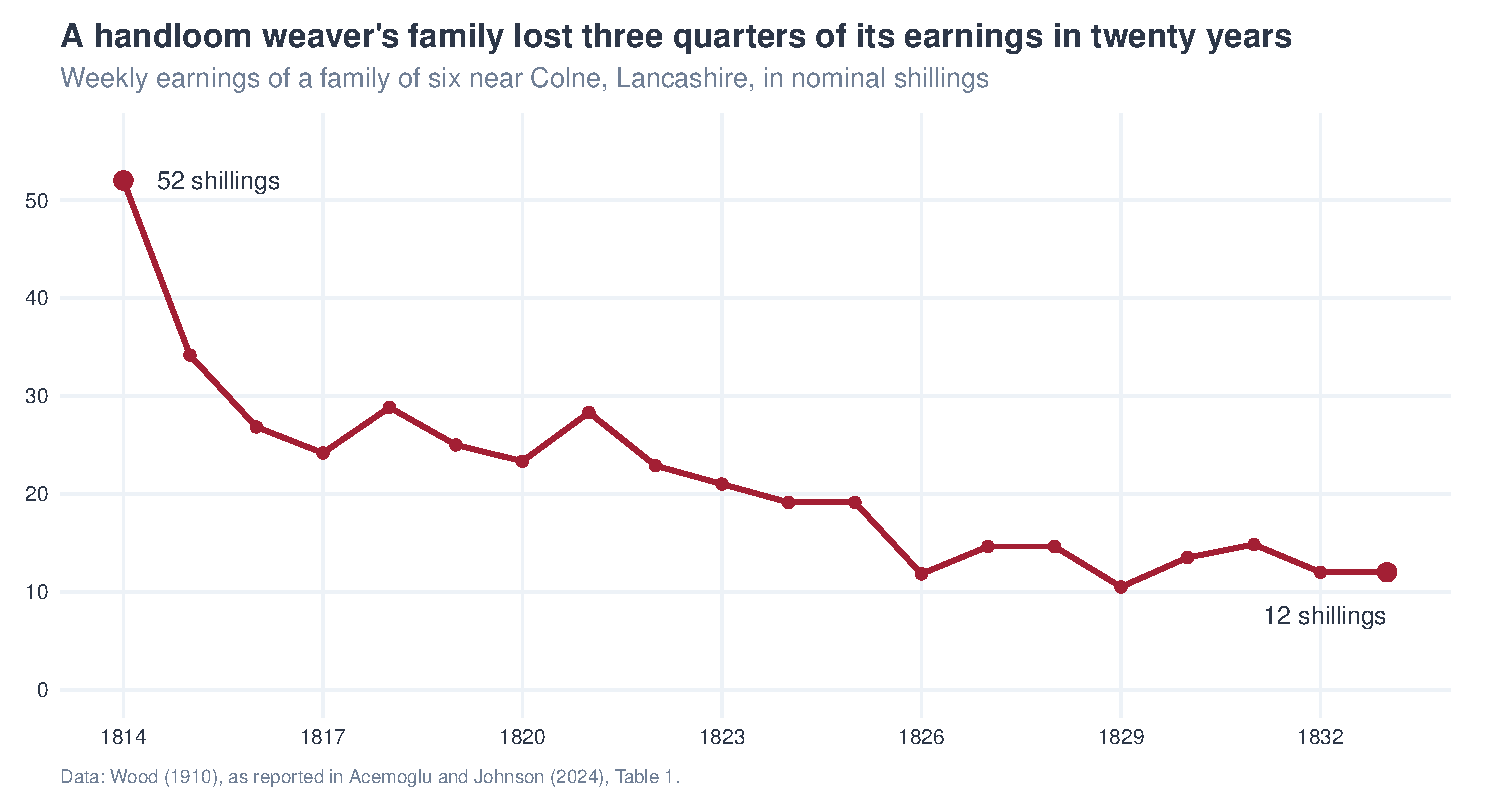
\includegraphics[width=\textwidth,height=0.78\textheight,keepaspectratio]{aj2024_handloom_earnings.pdf}
\end{center}
\end{frame}

\begin{frame}{Only later did the jobs go}
\begin{center}
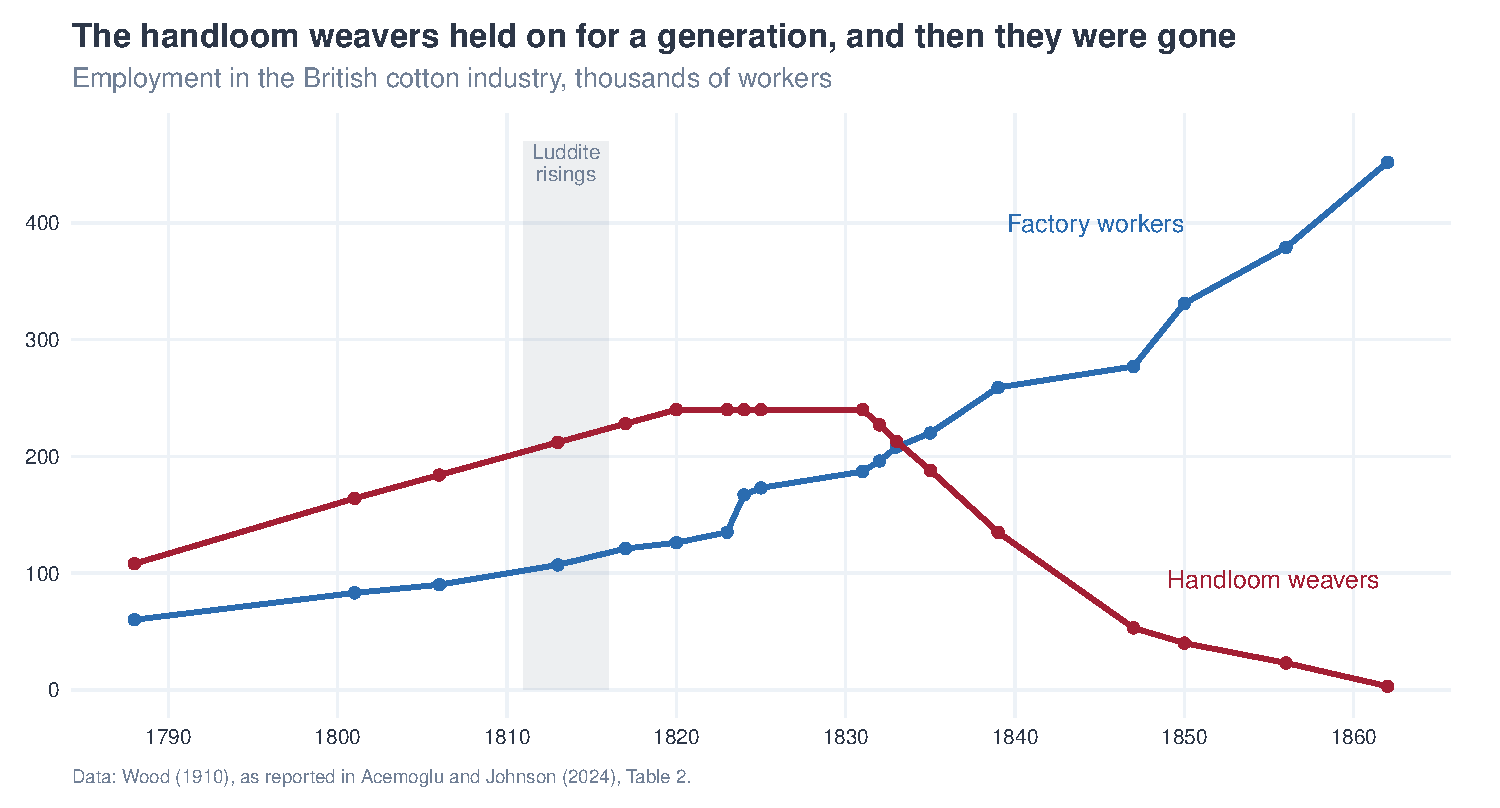
\includegraphics[width=\textwidth,height=0.78\textheight,keepaspectratio]{aj2024_cotton_employment.pdf}
\end{center}
\end{frame}

\begin{frame}{Wages adjusted for twenty years before employment did}

\begin{itemize}\setlength\itemsep{0.4em}
    \item A weaving family's earnings fell from 52 shillings a week to 12 between 1814 and 1833.
    \item Over those same years the number of handloom weavers did not fall. It stayed at its peak of 240,000.
    \item They worked longer for less: by the 1830s, fourteen to sixteen hours a day, six days a week.
    \item Their real wage fell to about a quarter of what it had been.
    \item The jobs disappeared afterward, from 240,000 in 1831 to 3,000 in 1862.
\end{itemize}

\vspace{0.35cm}

\alert{If you look only at employment, you miss the first twenty years of the story.}

\vspace{0.05cm}
{\scriptsize\color{warmgray}Acemoglu and Johnson (2024), Tables 1 and 2, from Wood (1910).}

\end{frame}

\begin{frame}{David Ricardo changed his mind}

\begin{center}
\footnotesize
\begin{tabular}{@{}ll@{}}
\toprule
\textbf{1817} & In the first edition of his \emph{Principles}, machinery does workers no harm. \\
\textbf{1819} & He tells Parliament that ``machinery did not lessen the demand for labor.'' \\
\textbf{1819} & Peterloo: a reform meeting of perhaps 60,000 in Manchester is broken up by force. \\
\textbf{1821} & The third edition adds a chapter, ``On Machinery.'' \\
\bottomrule
\end{tabular}
\end{center}

\vspace{0.3cm}

In that chapter he wrote that his opinions had ``undergone a considerable change.''

\vspace{0.3cm}

\alert{The best economist of his day got it wrong in real time, saw the evidence, and said so in print.}

\vspace{0.05cm}
{\scriptsize\color{warmgray}Acemoglu and Johnson (2024).}

\end{frame}

\begin{frame}{Shared gains came later, from new tasks and from worker voice}

\begin{itemize}\setlength\itemsep{0.4em}
    \item Real wages across the British economy were roughly flat until the 1830s.
    \item The average wage in cotton stayed below its 1806 level through 1862.
    \item By many estimates, the recovery took longer than a working lifetime.
\end{itemize}

\vspace{0.25cm}

\textbf{What changed after about 1850}
\begin{itemize}\setlength\itemsep{0.3em}
    \item Railways and heavy industry created tasks that had not existed.
    \item The vote widened, and unions won the right to bargain.
\end{itemize}

\vspace{0.3cm}

\alert{Acemoglu and Johnson's reading: none of it was preordained. ``These were choices.''}

\vspace{0.05cm}
{\scriptsize\color{warmgray}Acemoglu and Johnson (2024).}

\end{frame}

% ---- TAMU NEW (2026-10-01): Anna Karenina principle + Shockley (slides from amleds_deck.tex, June 2026) ----
\begin{frame}{Research is an Anna Karenina problem}

\begin{center}
{\large\itshape ``Happy families are all alike; every unhappy family is unhappy in its own way.''}

\vspace{0.1cm}
{\small\color{warmgray}Tolstoy, \emph{Anna Karenina}}
\end{center}

\vspace{0.3cm}

\begin{itemize}\setlength\itemsep{0.35em}
    \item A happy family needs five or six things, and it needs every one of them.
    \item Being excellent at four does not make up for the one that is missing.
    \item A mousetrap is the same: take away any one part and it catches nothing.
\end{itemize}

\vspace{0.35cm}

\alert{Good research is like a happy family. It succeeds one way, with everything present, and it can fail in many ways.}

\end{frame}

\begin{frame}{Shockley had a production function for science}

In 1957, William Shockley wrote ``On the Statistics of Individual Variations of Productivity in Research Laboratories.''

\vspace{0.25cm}

He argued that research productivity has a long-tailed, log-normal shape: a small number of workers produce enormously more measurable output.

\vspace{0.25cm}

\begin{center}
\[
P = F_1F_2F_3F_4F_5F_6F_7F_8
\qquad\Rightarrow\qquad
\log P = \sum_{j=1}^8 \log F_j
\]
\end{center}

\vspace{0.15cm}

He did not call it a production function, but that is what it is. In our language it is Cobb--Douglas: set any one input to zero and output is zero.

\end{frame}

\begin{frame}{Shockley's inputs mix production and verification}

In 1957, these were bundled inside the research worker. With agents, they begin to separate.

\vspace{0.08cm}

\begin{center}
\scriptsize
\renewcommand{\arraystretch}{1.05}
\begin{tabular}{@{}p{0.48\textwidth}ccl@{}}
\toprule
Shockley's factor & Task & & Agent pressure \\
\midrule
Think of a good problem & B & \textcolor{forest}{\Large $\uparrow$} & search, recombination \\
Work on it & P & \textcolor{forest}{\Large $\uparrow$} & tireless execution \\
Recognize a worthwhile result & B & \textcolor{mitcardinal}{\Large $\downarrow$} & if attention is outsourced \\
Know when to stop and write & B & \textcolor{warmgray}{\Large $\leftrightarrow$} & still judgment \\
Write adequately & P & \textcolor{forest}{\Large $\uparrow$} & drafting, editing \\
Profit from criticism & B & \textcolor{forest}{\Large $\uparrow$} & referee simulation \\
Submit to a journal & B & \textcolor{warmgray}{\Large $\leftrightarrow$} & incentives remain human \\
Persist through revisions & B & \textcolor{forest}{\Large $\uparrow$} & cheap iteration \\
\bottomrule
\end{tabular}
\end{center}

\vspace{0.05cm}
\textcolor{warmgray}{\scriptsize P = mostly production, B = bundled production and verification}

\vspace{0.08cm}
\alert{The new skill is harnessing both sides through trial, error, and experimentation.}

\end{frame}

\begin{frame}{Because it multiplies, your smallest input caps your output}

Output is the \emph{product} of eight inputs, not their sum:

\vspace{0.1cm}
\begin{center}
\[
P = F_1 F_2 F_3 F_4 F_5 F_6 F_7 F_8
\]
\end{center}
\vspace{0.02cm}

Find a problem, work on it, recognize a result, know when to stop, write it up, profit from criticism, submit it, persist through revision.

\vspace{0.18cm}

{\footnotesize\color{warmgray} His own illustration: a worker 50\% better on \emph{each} of the eight factors is about \textbf{25$\times$} as productive ($1.5^{8}\approx 25$).}

\vspace{0.18cm}

\alert{The binding input is different for each of us. That is every unhappy family, unhappy in its own way.}

\end{frame}

\begin{frame}{The eight inputs have not changed. Who supplies them has.}

\begin{itemize}\setlength\itemsep{0.4em}
    \item Agents can now supply several of Shockley's inputs, and supply them cheaply.
    \item Every one of the eight still has to be present.
    \item If an agent does the work and nobody recognizes whether the result is worthwhile, the product is still zero.
\end{itemize}

\vspace{0.35cm}

Learning to ride this new bull is going to be a challenge, and each of us will fall off in a different place.

\vspace{0.3cm}

\alert{But I think Shockley was right. The inputs to good research in 2026 are the inputs he listed in 1957.}

\end{frame}

\begin{frame}{What I am sure of: the human in the loop is essential}

I do not know whether we are complements or substitutes, or who will be hollowed out.

\vspace{0.3cm}

\textbf{What my own research on agents doing causal inference tells me}
\begin{itemize}\setlength\itemsep{0.3em}
    \item Agents take actions you did not ask for.
    \item The finished output does not show that they did.
    \item Those hidden actions can change the answer.
\end{itemize}

\vspace{0.3cm}

So someone who understands the work has to check it, every time.

\vspace{0.3cm}

\alert{Whether people know that yet is another matter. I am convinced of it.}

\end{frame}

{
\setbeamercolor{background canvas}{bg=charcoal}
\begin{frame}[plain]
\vfill
\begin{center}
{\color{lightbg}\Huge\bfseries Production is cheap.}\\[0.4cm]
{\color{lightbg}\Huge\bfseries Verification is the craft.}

\vspace{1.0cm}
{\color{warmgray}\rule{3cm}{0.5pt}}

\vspace{0.6cm}
{\color{lightbg}\large Scott Cunningham}\\[2pt]
{\color{warmgray} Baylor University \quad$\cdot$\quad \texttt{causalinf.substack.com}}
\end{center}
\vfill
\end{frame}
}

\end{document}
